% Options for packages loaded elsewhere
\PassOptionsToPackage{unicode}{hyperref}
\PassOptionsToPackage{hyphens}{url}
%
\documentclass[
]{book}
\usepackage{amsmath,amssymb}
\usepackage{lmodern}
\usepackage{iftex}
\ifPDFTeX
  \usepackage[T1]{fontenc}
  \usepackage[utf8]{inputenc}
  \usepackage{textcomp} % provide euro and other symbols
\else % if luatex or xetex
  \usepackage{unicode-math}
  \defaultfontfeatures{Scale=MatchLowercase}
  \defaultfontfeatures[\rmfamily]{Ligatures=TeX,Scale=1}
\fi
% Use upquote if available, for straight quotes in verbatim environments
\IfFileExists{upquote.sty}{\usepackage{upquote}}{}
\IfFileExists{microtype.sty}{% use microtype if available
  \usepackage[]{microtype}
  \UseMicrotypeSet[protrusion]{basicmath} % disable protrusion for tt fonts
}{}
\makeatletter
\@ifundefined{KOMAClassName}{% if non-KOMA class
  \IfFileExists{parskip.sty}{%
    \usepackage{parskip}
  }{% else
    \setlength{\parindent}{0pt}
    \setlength{\parskip}{6pt plus 2pt minus 1pt}}
}{% if KOMA class
  \KOMAoptions{parskip=half}}
\makeatother
\usepackage{xcolor}
\usepackage{color}
\usepackage{fancyvrb}
\newcommand{\VerbBar}{|}
\newcommand{\VERB}{\Verb[commandchars=\\\{\}]}
\DefineVerbatimEnvironment{Highlighting}{Verbatim}{commandchars=\\\{\}}
% Add ',fontsize=\small' for more characters per line
\usepackage{framed}
\definecolor{shadecolor}{RGB}{248,248,248}
\newenvironment{Shaded}{\begin{snugshade}}{\end{snugshade}}
\newcommand{\AlertTok}[1]{\textcolor[rgb]{0.94,0.16,0.16}{#1}}
\newcommand{\AnnotationTok}[1]{\textcolor[rgb]{0.56,0.35,0.01}{\textbf{\textit{#1}}}}
\newcommand{\AttributeTok}[1]{\textcolor[rgb]{0.77,0.63,0.00}{#1}}
\newcommand{\BaseNTok}[1]{\textcolor[rgb]{0.00,0.00,0.81}{#1}}
\newcommand{\BuiltInTok}[1]{#1}
\newcommand{\CharTok}[1]{\textcolor[rgb]{0.31,0.60,0.02}{#1}}
\newcommand{\CommentTok}[1]{\textcolor[rgb]{0.56,0.35,0.01}{\textit{#1}}}
\newcommand{\CommentVarTok}[1]{\textcolor[rgb]{0.56,0.35,0.01}{\textbf{\textit{#1}}}}
\newcommand{\ConstantTok}[1]{\textcolor[rgb]{0.00,0.00,0.00}{#1}}
\newcommand{\ControlFlowTok}[1]{\textcolor[rgb]{0.13,0.29,0.53}{\textbf{#1}}}
\newcommand{\DataTypeTok}[1]{\textcolor[rgb]{0.13,0.29,0.53}{#1}}
\newcommand{\DecValTok}[1]{\textcolor[rgb]{0.00,0.00,0.81}{#1}}
\newcommand{\DocumentationTok}[1]{\textcolor[rgb]{0.56,0.35,0.01}{\textbf{\textit{#1}}}}
\newcommand{\ErrorTok}[1]{\textcolor[rgb]{0.64,0.00,0.00}{\textbf{#1}}}
\newcommand{\ExtensionTok}[1]{#1}
\newcommand{\FloatTok}[1]{\textcolor[rgb]{0.00,0.00,0.81}{#1}}
\newcommand{\FunctionTok}[1]{\textcolor[rgb]{0.00,0.00,0.00}{#1}}
\newcommand{\ImportTok}[1]{#1}
\newcommand{\InformationTok}[1]{\textcolor[rgb]{0.56,0.35,0.01}{\textbf{\textit{#1}}}}
\newcommand{\KeywordTok}[1]{\textcolor[rgb]{0.13,0.29,0.53}{\textbf{#1}}}
\newcommand{\NormalTok}[1]{#1}
\newcommand{\OperatorTok}[1]{\textcolor[rgb]{0.81,0.36,0.00}{\textbf{#1}}}
\newcommand{\OtherTok}[1]{\textcolor[rgb]{0.56,0.35,0.01}{#1}}
\newcommand{\PreprocessorTok}[1]{\textcolor[rgb]{0.56,0.35,0.01}{\textit{#1}}}
\newcommand{\RegionMarkerTok}[1]{#1}
\newcommand{\SpecialCharTok}[1]{\textcolor[rgb]{0.00,0.00,0.00}{#1}}
\newcommand{\SpecialStringTok}[1]{\textcolor[rgb]{0.31,0.60,0.02}{#1}}
\newcommand{\StringTok}[1]{\textcolor[rgb]{0.31,0.60,0.02}{#1}}
\newcommand{\VariableTok}[1]{\textcolor[rgb]{0.00,0.00,0.00}{#1}}
\newcommand{\VerbatimStringTok}[1]{\textcolor[rgb]{0.31,0.60,0.02}{#1}}
\newcommand{\WarningTok}[1]{\textcolor[rgb]{0.56,0.35,0.01}{\textbf{\textit{#1}}}}
\usepackage{longtable,booktabs,array}
\usepackage{calc} % for calculating minipage widths
% Correct order of tables after \paragraph or \subparagraph
\usepackage{etoolbox}
\makeatletter
\patchcmd\longtable{\par}{\if@noskipsec\mbox{}\fi\par}{}{}
\makeatother
% Allow footnotes in longtable head/foot
\IfFileExists{footnotehyper.sty}{\usepackage{footnotehyper}}{\usepackage{footnote}}
\makesavenoteenv{longtable}
\usepackage{graphicx}
\makeatletter
\def\maxwidth{\ifdim\Gin@nat@width>\linewidth\linewidth\else\Gin@nat@width\fi}
\def\maxheight{\ifdim\Gin@nat@height>\textheight\textheight\else\Gin@nat@height\fi}
\makeatother
% Scale images if necessary, so that they will not overflow the page
% margins by default, and it is still possible to overwrite the defaults
% using explicit options in \includegraphics[width, height, ...]{}
\setkeys{Gin}{width=\maxwidth,height=\maxheight,keepaspectratio}
% Set default figure placement to htbp
\makeatletter
\def\fps@figure{htbp}
\makeatother
\setlength{\emergencystretch}{3em} % prevent overfull lines
\providecommand{\tightlist}{%
  \setlength{\itemsep}{0pt}\setlength{\parskip}{0pt}}
\setcounter{secnumdepth}{5}
\usepackage{booktabs}
\ifLuaTeX
  \usepackage{selnolig}  % disable illegal ligatures
\fi
\usepackage[]{natbib}
\bibliographystyle{plainnat}
\IfFileExists{bookmark.sty}{\usepackage{bookmark}}{\usepackage{hyperref}}
\IfFileExists{xurl.sty}{\usepackage{xurl}}{} % add URL line breaks if available
\urlstyle{same} % disable monospaced font for URLs
\hypersetup{
  pdftitle={MEPS tutorials},
  pdfauthor={Mark Bounthavong},
  hidelinks,
  pdfcreator={LaTeX via pandoc}}

\title{MEPS tutorials}
\author{Mark Bounthavong}
\date{2024-01-21}

\begin{document}
\maketitle

{
\setcounter{tocdepth}{1}
\tableofcontents
}
\hypertarget{about}{%
\chapter*{About}\label{about}}
\addcontentsline{toc}{chapter}{About}

This is a collection of tutorials that use data from the Agency for Healthcare Research and Quality (AHRQ) \href{https://meps.ahrq.gov/mepsweb/}{Medical Expenditure Panel Survey (MEPS)}.

These tutorials use \href{https://cran.r-project.org/}{R} and \href{https://posit.co/products/open-source/rstudio/}{RStudio} for data loading, manipulation, analysis, and presentation.

\hypertarget{book-link}{%
\section*{Book link}\label{book-link}}
\addcontentsline{toc}{section}{Book link}

The GitHub link to the MEPS tutorials collection: \url{https://mbounthavong.github.io/MEPS_tutorials_book/}

\hypertarget{table-of-contents}{%
\section*{Table of contents}\label{table-of-contents}}
\addcontentsline{toc}{section}{Table of contents}

Chapter \protect\hyperlink{intro}{1} provides an introduction on how to load and import MEPS data into R.

Chapter \protect\hyperlink{merging}{2} is an instruction on how to merge various MEPS data files.

Chapter \protect\hyperlink{weights}{3} focuses on applying weights to the population.

Chapter \protect\hyperlink{clnk}{4} using condition-event link file

Chapter \protect\hyperlink{trends}{5} simple trend analysis with linear models

Chapter \protect\hyperlink{itsa}{6} interrupted time series analysis

Chapter \protect\hyperlink{notes}{7} helpful notes

Further chapters are forthcoming.

\hypertarget{intro}{%
\chapter{Loading MEPS data into R}\label{intro}}

\hypertarget{introduction}{%
\section{Introduction}\label{introduction}}

The Agency for Healthcare Research and Quality (AHRQ) \href{https://www.meps.ahrq.gov/mepsweb/}{Medical Expenditure Panel Survey (MEPS)} is a set of data on U.S. households about their healthcare expenditures. It includes data on the individual / household demographics, socioeconomic status, insurance coverage, and healthcare expenditures. Healthcare expenditures include data on health-related spending, medical conditions, prescriptions, and utilization (e.g., number of office-based visits). MEPS draws upon a nationally representative subsample from the \href{https://www.cdc.gov/nchs/nhis/index.htm?CDC_AA_refVal=https\%3A\%2F\%2Fwww.cdc.gov\%2Fnchs\%2Fnhis.htm}{National Health Interview Survey}, which is conducted by the \href{https://www.cdc.gov/nchs/index.htm}{National Center for Health Statistics}. Hence, MEPS provides researchers with the ability to generate estimates for the representative U.S. population.

\hypertarget{meps-data}{%
\section{MEPS Data}\label{meps-data}}

MEPS data are located on their website in their \href{https://www.meps.ahrq.gov/mepsweb/data_stats/download_data_files.jsp}{data files page}. You can find data from 1996 to the most recent available year (during the writing of this tutorial, 2020 was the latest release).

\begin{figure}
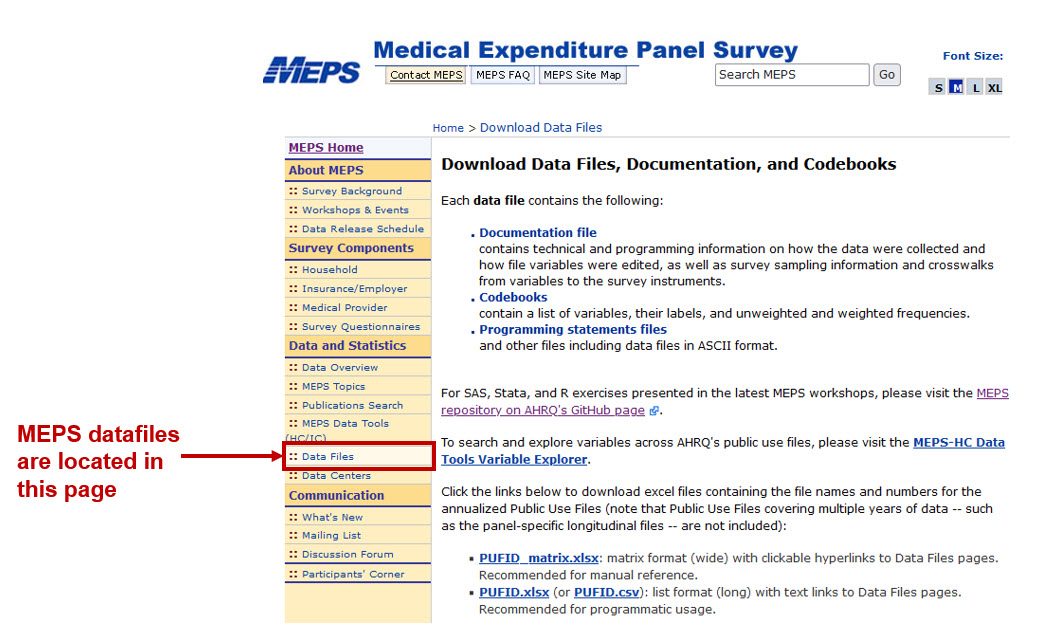
\includegraphics[width=1\linewidth]{Figure 1} \caption{Figure 1 - Location of MEPS data files}\label{fig:unnamed-chunk-2}
\end{figure}

The MEPS data files include the \href{https://www.meps.ahrq.gov/mepsweb/data_stats/download_data_files_detail.jsp?cboPufNumber=HC-224}{Full-Year Consolidated Data files}, which is the calendar-year summary of the different longitudinal panels. The Full-Year Consolidated Data files contain information on the annual healthcare expenditures by the type of care; it contains data on spending, insurance coverage, health status, patient satisfaction, and several health conditions. The Full-Year Consolidated Data files also contains information from several surveys (e.g,. Diabetes Care Survey).

\begin{figure}
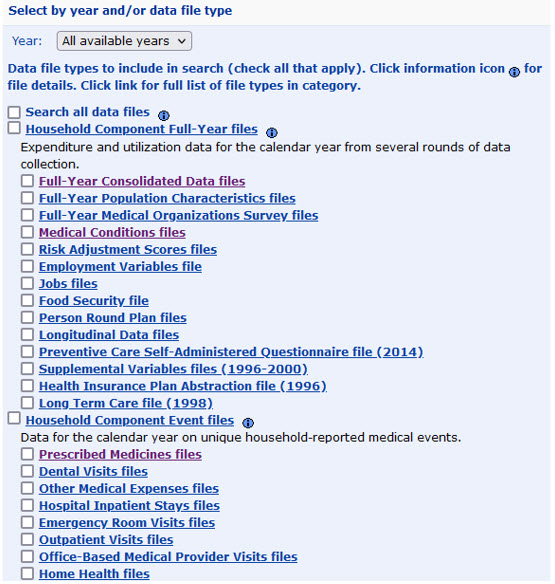
\includegraphics[width=1\linewidth]{Figure 2} \caption{Figure 2 - Full-Year Consolidated Data files and other data types}\label{fig:unnamed-chunk-3}
\end{figure}

\hypertarget{load-meps-data-into-r}{%
\section{Load MEPS data into R}\label{load-meps-data-into-r}}

MEPS data can be downloaded onto your local storage and read into a statistical software program such as Stata or R. But you can also communicate directly with the AHRQ MEPS website to load your data rather than having to download it. We will load the Full-Year Consolidated Data file from 2020, which is named \texttt{HC-224}. To find out the name of the file, you will need to go MEPS data files site and click on the Full-Year Consolidated Data files. In this page (Figure 2), you can see the data file with the code \texttt{HC-224}, which is the Full-Year Consolidated Data file for 2020. When we enter this into our R code, we will use the file name \texttt{h224}.

\begin{figure}
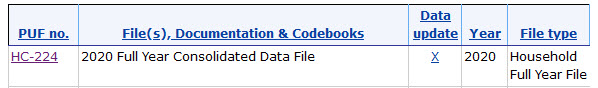
\includegraphics[width=1\linewidth]{Figure 3} \caption{Figure 3 - H224 is the MEP 2020 Full-Year Consolidated Data file.}\label{fig:unnamed-chunk-4}
\end{figure}

You will need to download and install the \href{https://github.com/e-mitchell/meps_r_pkg}{\texttt{MEPS} package}. The \texttt{MEPS} package will provide tools for you to load and manipulate the MEPS Data files. You will need to have R \texttt{devtools} package installed.

\begin{Shaded}
\begin{Highlighting}[]
\DocumentationTok{\#\# Install the devtools package}
\CommentTok{\# install.packages("devtools") \#\# You only need to install this once}
\CommentTok{\# library("devtools")  \#\# You will need to reload the MEPS package each time you restart R}
\CommentTok{\# install\_github("e{-}mitchell/meps\_r\_pkg/MEPS") \#\# This will install the MEPS package for R}
\end{Highlighting}
\end{Shaded}

There are two methods to load MEPS data into R.

Method 1 requires that you know the file name. In this example, the MEPS 2020 Full-Year Consolidated Data file is named \texttt{h224}. We will use the \texttt{read\_MEPS} function to load the MEPS data onto R.

When using Method 2 to load the MEPS data, we don't need to know the file name, but we need to know the year and the data type. For example, for the Full-Year Consolidated Data file, we use the \texttt{year\ =\ 2020} and \texttt{type\ =\ "FYC"} option. For this method, we will also use the \texttt{read\_MEPS} function to the MEPS data onto R.

The \texttt{tolower} function is used to change all the variable names from upper case to lower case. MEPS defaults the column names to upper case. I like to change this to lower case because it's easier for me to type.

\begin{Shaded}
\begin{Highlighting}[]
\DocumentationTok{\#\#\# Load the MEPS package}
\FunctionTok{library}\NormalTok{(}\StringTok{"MEPS"}\NormalTok{) }\DocumentationTok{\#\# You need to load the library every time you restart R}

\DocumentationTok{\#\#\#\# Method 1: Load data from AHRQ MEPS website}
\NormalTok{hc2020 }\OtherTok{=} \FunctionTok{read\_MEPS}\NormalTok{(}\AttributeTok{file =} \StringTok{"h224"}\NormalTok{)}

\DocumentationTok{\#\#\#\# Method 2: Load data from AHRQ MEPS website}
\NormalTok{hc2020 }\OtherTok{=} \FunctionTok{read\_MEPS}\NormalTok{(}\AttributeTok{year =} \DecValTok{2020}\NormalTok{, }\AttributeTok{type =} \StringTok{"FYC"}\NormalTok{)}

\DocumentationTok{\#\# Change column names to lowercase}
\FunctionTok{names}\NormalTok{(hc2020) }\OtherTok{\textless{}{-}} \FunctionTok{tolower}\NormalTok{(}\FunctionTok{names}\NormalTok{(hc2020))}
\end{Highlighting}
\end{Shaded}

There are over 1400 variables in the MEPS 2020 Full-Year Consolidated Data file. We can reduce this to the essential variables using the \texttt{subset} function. This will generate a smaller data frame that we will call \texttt{keep\_meps}. The variables that we want to collect are the subject unique identifier (\texttt{dupersid}), the survey weights (\texttt{varpsu}, \texttt{varstr}, \texttt{perwt20f}), and the total healthcare expenditures for 2020 (\texttt{totexp20}).

\begin{Shaded}
\begin{Highlighting}[]
\DocumentationTok{\#\#\# Keep the subject\textquotesingle{}s unique ID, survey weights, and total expenditures}
\NormalTok{keep\_meps }\OtherTok{\textless{}{-}} \FunctionTok{subset}\NormalTok{(hc2020, }\AttributeTok{select =} \FunctionTok{c}\NormalTok{(dupersid, varpsu, varstr, perwt20f, totexp20))}

\FunctionTok{head}\NormalTok{(keep\_meps) }\DocumentationTok{\#\# View the first six rows of the data frame}
\end{Highlighting}
\end{Shaded}

\begin{verbatim}
## # A tibble: 6 x 5
##   dupersid   varpsu varstr perwt20f totexp20
##   <chr>       <dbl>  <dbl>    <dbl>    <dbl>
## 1 2320005101      1   2079    8418.      459
## 2 2320005102      1   2079    5200.      564
## 3 2320006101      1   2028    2140.      140
## 4 2320006102      1   2028    2216.     4673
## 5 2320006103      1   2028    4157.      410
## 6 2320012102      2   2069    1961.     2726
\end{verbatim}

Since MEPS uses a complex survey design, these weights are needed to estimate standard errors that are reflective of the representative sample of the U.S. population. We'll learn how to apply these survey weights to the MEPS data files in a future tutorial.

\hypertarget{conclusions}{%
\section{Conclusions}\label{conclusions}}

Loading MEPS data into R allows us to perform analysis easily and quickly. In this tutorial, you learned how to load MEPS data into R directly from the MEPS website. However, you can also download the MEPS data onto your local storage and use the \texttt{setwd} command to set the working directory.

In future tutorials, we'll learn how to apply the survey weights and perform descriptive analyses using the MEPS data files.

\hypertarget{acknowledgements}{%
\section{Acknowledgements}\label{acknowledgements}}

There are a lot of tutorials on how to use MEPS data with R. I found the \href{https://github.com/HHS-AHRQ/MEPS}{AHRQ MEPS GitHub page} to be an invaluable resource.

This is a work in progress, and I may update this in the future.

\hypertarget{merging}{%
\chapter{Merging files}\label{merging}}

\hypertarget{introduction-1}{%
\section{Introduction}\label{introduction-1}}

We want to merge the Full-Year Consolidated Data file with the Medical Conditions file so that we can identify patients with a diagnosis of diabetes.

\hypertarget{load-meps-data}{%
\section{Load MEPS data}\label{load-meps-data}}

We need to lead the MEPS Full-Year Consolidated Data file and the Medical Conditions file from 2020. There are two methods to loading MEPS data into R. Method 1 requires you to know the name of the file. For example, the Medical Conditions file from 2020 is named \texttt{h222}. In Method 2, you need to know the \texttt{type\ =} of data you want to load. For example, the Medical Conditions file is named \texttt{CONDITIONS}.

I like to work with column names that are in the lower case, so I used the \texttt{tolower} function to change the column names from upper case to lower case.

\begin{Shaded}
\begin{Highlighting}[]
\DocumentationTok{\#\#\# Load the MEPS package}
\FunctionTok{library}\NormalTok{(}\StringTok{"MEPS"}\NormalTok{) }\DocumentationTok{\#\# You need to load the library every time you restart R}

\DocumentationTok{\#\#\#\# Method 1: Load data from AHRQ MEPS website}
\NormalTok{hc2020 }\OtherTok{=} \FunctionTok{read\_MEPS}\NormalTok{(}\AttributeTok{file =} \StringTok{"h224"}\NormalTok{)}
\NormalTok{mc2020 }\OtherTok{=} \FunctionTok{read\_MEPS}\NormalTok{(}\AttributeTok{file =} \StringTok{"h222"}\NormalTok{)}

\DocumentationTok{\#\#\#\# Method 2: Load data from AHRQ MEPS website}
\NormalTok{hc2020 }\OtherTok{=} \FunctionTok{read\_MEPS}\NormalTok{(}\AttributeTok{year =} \DecValTok{2020}\NormalTok{, }\AttributeTok{type =} \StringTok{"FYC"}\NormalTok{)}
\NormalTok{mc2020 }\OtherTok{=} \FunctionTok{read\_MEPS}\NormalTok{(}\AttributeTok{year =} \DecValTok{2020}\NormalTok{, }\AttributeTok{type =} \StringTok{"CONDITIONS"}\NormalTok{)}

\DocumentationTok{\#\# Change column names to lowercase}
\FunctionTok{names}\NormalTok{(hc2020) }\OtherTok{\textless{}{-}} \FunctionTok{tolower}\NormalTok{(}\FunctionTok{names}\NormalTok{(hc2020))}
\FunctionTok{names}\NormalTok{(mc2020) }\OtherTok{\textless{}{-}} \FunctionTok{tolower}\NormalTok{(}\FunctionTok{names}\NormalTok{(mc2020))}
\end{Highlighting}
\end{Shaded}

\hypertarget{merge-meps-data}{%
\section{Merge MEPS data}\label{merge-meps-data}}

Now that we have both the \texttt{h224} and \texttt{h222} file loaded into R, we can marge these files together. The Full-Year Consolidated Data file contains unique patients (e.g., each row is a unique patient); hence, the unique identifier \texttt{dupersid} is not repeatable. Figure 1 illustrates an example of a table with each row as a unique subject. Note how the \texttt{dupersid} does not repeat.

\begin{figure}
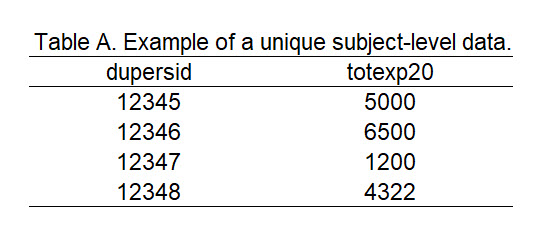
\includegraphics[width=0.8\linewidth]{Figure 2_1} \caption{Figure 1 - Example table with unique patients.}\label{fig:unnamed-chunk-9}
\end{figure}

However, in the Medical Conditions file, the rows are for the number of unique diagnosis grouped by the patient. In other words, the Medical Conditions file will contain repeated \texttt{dupersid} for each diagnosis. For example, a person can have 5 diagnosis grouped by their \texttt{dupersid}. In Figure 2, we have an example table with a subject \texttt{dupersid\ =\ 12345} who has five diagnosis (\texttt{icd10cdx}).

\begin{figure}
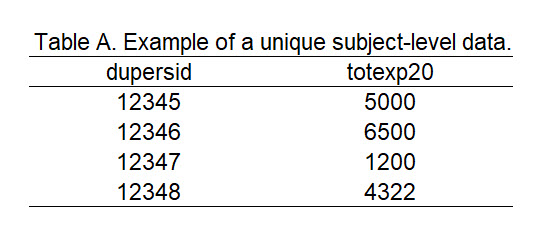
\includegraphics[width=1\linewidth]{Figure 2_1} \caption{Figure 2 - Example table where the unique patient identifier repeats.}\label{fig:unnamed-chunk-10}
\end{figure}

When we merge the Full-Year Consolidated Data file (which is unique to the \texttt{dupersid}) with the Medical Conditions file (which has repeatable \texttt{dupersid}), we will merge using a 1 to many merge (\texttt{Figure\ 3a}). \texttt{Figure\ 3a} illustrates the merge between the unique subject-level table to the repeatable subject-level table.

\begin{figure}
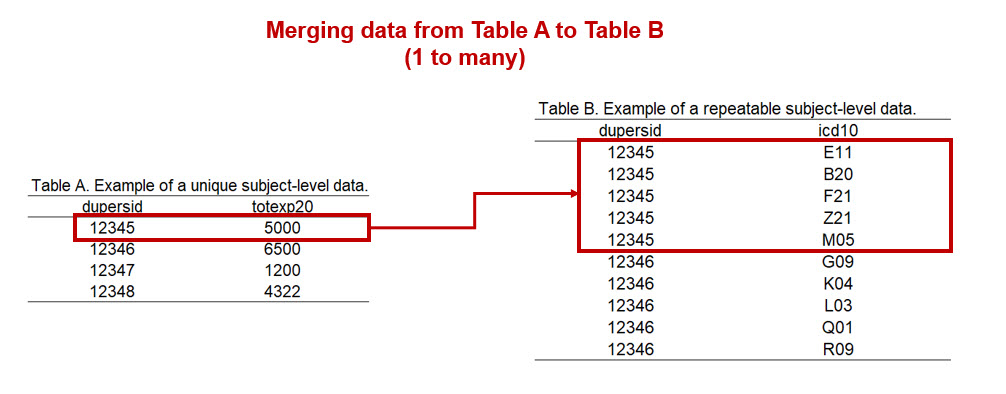
\includegraphics[width=1\linewidth]{Figure 2_3a} \caption{Figure 3a - Merging tables (1 to many).}\label{fig:unnamed-chunk-11}
\end{figure}

But we also want to make sure that we include all the patients in the Full-Year Consolidated Data file. Not all patients will have a diagnostic code, so we need to be careful that we don't accidentally drop them from the query. \texttt{Figure\ 3b} illustrates our intention to merge all the data from the Full-Year Consolidated Data file with some of the data from the Medical Conditions file.

\begin{figure}
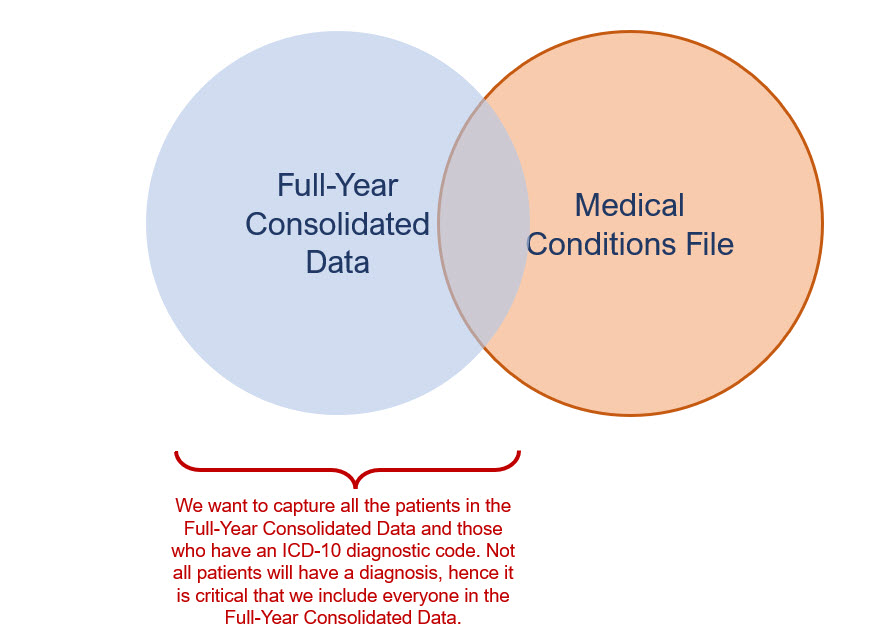
\includegraphics[width=1\linewidth]{Figure 2_3b} \caption{Figure 3b - Merging tables with all patients in the Full-Year Consolidated Data file and some of the data from the Medical Conditions file.}\label{fig:unnamed-chunk-12}
\end{figure}

Now that we understand how we want to merge the data, we can proceed to write the code.

There are two methods to merge the data files.

\textbf{Method 1:} We use the \texttt{merge} function to merge the two MEPS data files. The \texttt{by\ =} option is where we enter the matching variable \texttt{dupersid}. We will call the merged data set \texttt{total}. Using the `\texttt{merge} function, we are telling R that we want to do a 1 to many match between the Full-Year Consolidated Data file and the Medical Conditions file using the \texttt{dupersid} as the matching variable. We have to include the \texttt{all.x\ =\ TRUE} argument because we want to make sure we include the patients without any diagnostic codes.

\begin{Shaded}
\begin{Highlighting}[]
\DocumentationTok{\#\# MERGE data {-} Medical conditions and household component}
\CommentTok{\# merge two data frames by ID; there are two methods to do this:}

\DocumentationTok{\#\#\#\# Method 1: Native R function; Note: all.x means that we pull all dupersid, even the ones that don\textquotesingle{}t have a medical condition)}
\NormalTok{total }\OtherTok{\textless{}{-}} \FunctionTok{merge}\NormalTok{(hc2020, mc2020, }\AttributeTok{by =} \StringTok{"dupersid"}\NormalTok{, }\AttributeTok{all.x =} \ConstantTok{TRUE}\NormalTok{)}
\end{Highlighting}
\end{Shaded}

\textbf{Method 2:} We use the \texttt{left\_join} function from the \texttt{dplyr} package to merge the two MEPS data files. The \texttt{by\ =} option is where we enter the matching variable \texttt{dupersid}. We will call the merged data set \texttt{total}. Using the \texttt{left\_join} function, we are telling R that we want to do a 1 to many match between the Full-Year Consolidated Data file and the Medical Conditions file using the \texttt{dupersid} as the matching variable. The \texttt{left\_join} function is based on the SQL language syntax and operates in the same manner.

\begin{Shaded}
\begin{Highlighting}[]
\DocumentationTok{\#\#\#\# Method 2: Use SQL syntax (left\_join)}
\FunctionTok{library}\NormalTok{(}\StringTok{"dplyr"}\NormalTok{)}
\NormalTok{total }\OtherTok{\textless{}{-}} \FunctionTok{left\_join}\NormalTok{(hc2020, mc2020, }\AttributeTok{by =} \StringTok{"dupersid"}\NormalTok{)}
\end{Highlighting}
\end{Shaded}

Once the two data files are merged, we will have a data frame with repeatable \texttt{dupersid}. Notice that the \texttt{totexp20} variable from Table A is merged along with the \texttt{icd10} variable from Table B.

\begin{figure}
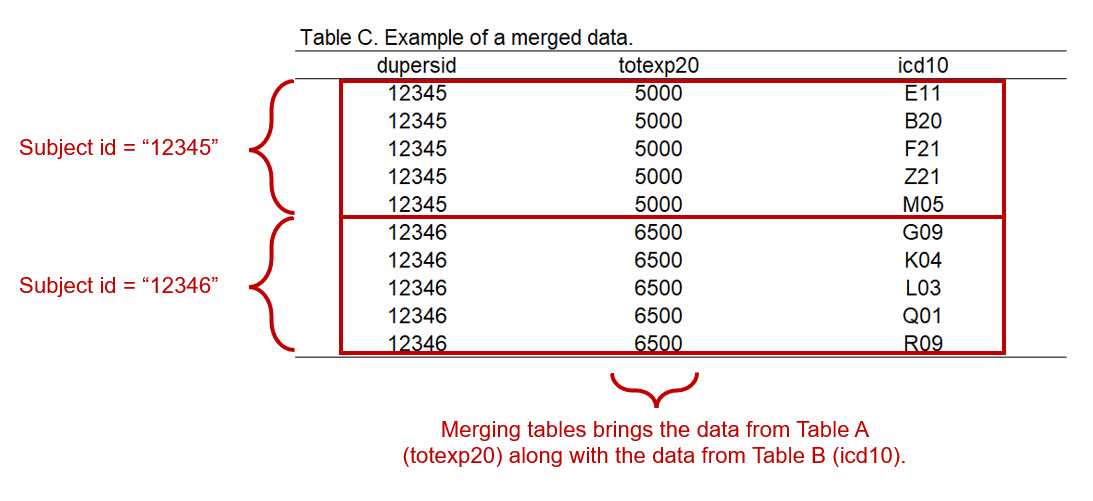
\includegraphics[width=1\linewidth]{Figure 2_4} \caption{Figure 4 - Merging data from Table A to Table B.}\label{fig:unnamed-chunk-15}
\end{figure}

\hypertarget{reduce-dataframe-to-a-few-variables}{%
\section{Reduce dataframe to a few variables}\label{reduce-dataframe-to-a-few-variables}}

Our \texttt{total} dataframe has 1481 variables and 80,802 observations. We want to make this dataframe manageable, so we'll create a limited dataframe with only the variables we're interested in. To do this, we'll use the \texttt{subset()} function.

For this exercise, we'll keep the \texttt{dupersid}, \texttt{varpsu.x}, \texttt{varsry.x}, \texttt{perwt20f.x}, and \texttt{icd10cdx} variables by using the \texttt{subset()} function. We'll call our reduced dataframe \texttt{keep\_mep2}. (Note: The \texttt{*.x} indicates the table on the left. We want to keep the \texttt{varpsu}, \texttt{varstr}, and \texttt{perwt20f} from the \texttt{hc2020} table. The \texttt{mc2020} table has duplicate variables that are denoted by \texttt{*.y}.)

\begin{Shaded}
\begin{Highlighting}[]
\NormalTok{keep\_meps2 }\OtherTok{\textless{}{-}} \FunctionTok{subset}\NormalTok{(total, }\AttributeTok{select =} \FunctionTok{c}\NormalTok{(}\StringTok{"dupersid"}\NormalTok{, }\StringTok{"varpsu.x"}\NormalTok{, }\StringTok{"varstr.x"}\NormalTok{, }\StringTok{"perwt20f.x"}\NormalTok{, }\StringTok{"icd10cdx"}\NormalTok{))}
\end{Highlighting}
\end{Shaded}

\hypertarget{add-an-indicator-for-a-specific-icd10-diagnostic-code}{%
\section{Add an indicator for a specific ICD10 diagnostic code}\label{add-an-indicator-for-a-specific-icd10-diagnostic-code}}

Our data frame has multiple rows grouped by the patient's id (\texttt{dupersid}); these rows are based on the various ICD-10 diagnostic codes. For example, patient \texttt{12345} has 5 ICD-10 diagnostic codes; hence, they have 5 rows (\texttt{Figure\ 4}).

Suppose we want to generate a binary indicator to identify patients with an ICD-10 diagnosis for diabetes (\texttt{E11}). In our example (\texttt{Figure\ 4}), patient \texttt{12345} has an ICD10 code for diabetes (\texttt{E11}).

We can create an indicator variable that will be unique to the patient for having diabetes. What we want to see if a new variable that identifies a patients with the specific ICD-10 code of interest. \texttt{Figure\ 5} illustrates the indicator variable for diabetes as an additional column \texttt{diabetes\_indicator}.

\begin{figure}
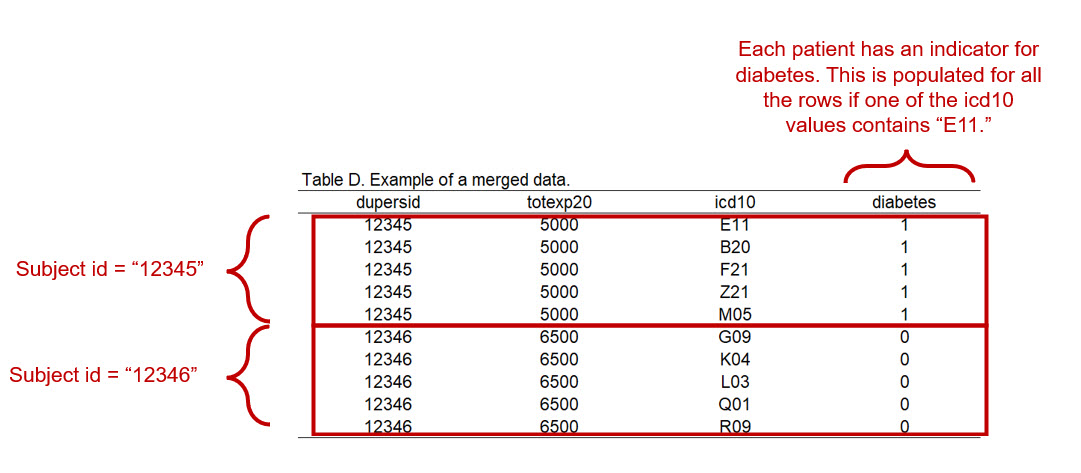
\includegraphics[width=1\linewidth]{Figure 2_5} \caption{Figure 5 - Indicator variable for diabetes.}\label{fig:unnamed-chunk-17}
\end{figure}

We create the indicator and call it \texttt{diabetes}, which is defined as \texttt{icd10cdx\ ==\ "E11"}. We will code this as \texttt{0} for no diabetes and \texttt{1} for diabetes. Then, we count the number of time a patient as \texttt{E11} in their \texttt{icd10cdx} column. I added the following option to the code (\texttt{\textbar{}\ is.na(total\$icd10cdx)}) because I want to make sure that all patients in the \texttt{total} table that do not have an ICD-10 code for \texttt{E11} is coded as \texttt{0}. There may be some patients that have \texttt{NA} or missing data in the \texttt{icd10cdx} variable. If the \texttt{icd10cdx} value is \texttt{NA}, this may not be coded with a \texttt{0}. Hence, we have to add the \texttt{\textbar{}\ is.na(total\$icd10cdx} code to ensure that we get a value of \texttt{0}.

\begin{Shaded}
\begin{Highlighting}[]
\DocumentationTok{\#\# Change to unique subject (each row is a unique subject)}
\DocumentationTok{\#\#\#\# Generate a variable to identify diabetes diagnosis for repeated rows}
\FunctionTok{library}\NormalTok{(}\StringTok{"tidyverse"}\NormalTok{)  }\DocumentationTok{\#\# Load tidyverse}

\NormalTok{keep\_meps2}\SpecialCharTok{$}\NormalTok{diabetes[total}\SpecialCharTok{$}\NormalTok{icd10cdx }\SpecialCharTok{!=} \StringTok{"E11"} \SpecialCharTok{|} \FunctionTok{is.na}\NormalTok{(total}\SpecialCharTok{$}\NormalTok{icd10cdx)] }\OtherTok{=} \DecValTok{0}
\NormalTok{keep\_meps2}\SpecialCharTok{$}\NormalTok{diabetes[total}\SpecialCharTok{$}\NormalTok{icd10cdx }\SpecialCharTok{==} \StringTok{"E11"}\NormalTok{] }\OtherTok{=} \DecValTok{1}

\FunctionTok{table}\NormalTok{(keep\_meps2}\SpecialCharTok{$}\NormalTok{diabetes) }\DocumentationTok{\#\# Visualize the number of patients with diabetes and no diabetes}
\end{Highlighting}
\end{Shaded}

\begin{verbatim}
## 
##     0     1 
## 87345  2693
\end{verbatim}

\begin{Shaded}
\begin{Highlighting}[]
\DocumentationTok{\#\#\# This code chunk calculates the number of times E11 appears for a unique patient}
\NormalTok{keep\_meps2 }\OtherTok{\textless{}{-}}\NormalTok{ keep\_meps2 }\SpecialCharTok{\%\textgreater{}\%}
  \FunctionTok{group\_by}\NormalTok{(dupersid) }\SpecialCharTok{\%\textgreater{}\%}
  \FunctionTok{mutate}\NormalTok{(}\AttributeTok{diabetes\_indicator =} \FunctionTok{sum}\NormalTok{(diabetes }\SpecialCharTok{==} \StringTok{"1"}\NormalTok{, }\AttributeTok{na.rm =} \ConstantTok{TRUE}\NormalTok{)) }\SpecialCharTok{\%\textgreater{}\%}
\NormalTok{  ungroup}
\FunctionTok{table}\NormalTok{(keep\_meps2}\SpecialCharTok{$}\NormalTok{diabetes\_indicator)}
\end{Highlighting}
\end{Shaded}

\begin{verbatim}
## 
##     0     1     2 
## 71804 17295   939
\end{verbatim}

According to our results, there were 17,295 events where a patient had one diagnostic code for \texttt{E11} and 939 events where a patient had two diagnostic codes for \texttt{E11}. How did this occur? MEPS public files only list the first three digits of the ICD-10 code to protect the identity of the patient. The ICD-10 diagnostic code has more digits beyond the first three. For example, an ICD-10 diagnosis for Type 2 diabetes with diabetic chronic kidney disease is \texttt{E11.22}. Hence, there will be patients with unique ICD-10 codes that may appear identical because only the first three digits are present in the MEPS public files.

In our example, we have patients with 1 and 2 ICD-10 diagnostic codes for \texttt{E11}. We would like to create a binary indicator of diabetes, so we need to take the current information and transform the variable \texttt{diabetes} in the \texttt{keep\_meps} dataframe into a new variable that only has \texttt{0} and \texttt{1}.

We can do this by combining the \texttt{mutate} function with the \texttt{ifelse} function. See the code below:

\begin{Shaded}
\begin{Highlighting}[]
\NormalTok{keep\_meps2 }\OtherTok{\textless{}{-}}\NormalTok{ keep\_meps2 }\SpecialCharTok{\%\textgreater{}\%} 
  \FunctionTok{group\_by}\NormalTok{(dupersid) }\SpecialCharTok{\%\textgreater{}\%}
  \FunctionTok{mutate}\NormalTok{(}\AttributeTok{diabetes\_binary =} \FunctionTok{ifelse}\NormalTok{(diabetes\_indicator }\SpecialCharTok{\textgreater{}=} \DecValTok{1}\NormalTok{, }\DecValTok{1}\NormalTok{, }\DecValTok{0}\NormalTok{), }\AttributeTok{na.rm =} \ConstantTok{TRUE}\NormalTok{) }\SpecialCharTok{\%\textgreater{}\%}
\NormalTok{  ungroup}
\FunctionTok{table}\NormalTok{(keep\_meps2}\SpecialCharTok{$}\NormalTok{diabetes\_binary)}
\end{Highlighting}
\end{Shaded}

\begin{verbatim}
## 
##     0     1 
## 71804 18234
\end{verbatim}

Now, we have a new binary indicator variable. The \texttt{diabetes\_binary} variable is coded \texttt{1} if the patient has the \texttt{E11} diagnostic code and \texttt{0} if the patient does not.

\hypertarget{collapse-dataframe-to-a-single-unique-patient}{%
\section{Collapse dataframe to a single unique patient}\label{collapse-dataframe-to-a-single-unique-patient}}

But since this is a dataframe with duplicated patients, we want to collapse this into a dataframe where each row is a single unique patient.

Since a lot of the variables in the dataframe are the same when grouped by the unique \texttt{dupersid}, we can estimate the mean and get the same value. For example, let's look at \texttt{Figure\ 5} again. For \texttt{dupersid\ ==\ 12345}, there are five values for \texttt{totexp20}, which are:

\begin{itemize}
\item
  \texttt{5000} when \texttt{icd10} is \texttt{E11},
\item
  \texttt{5000} when \texttt{icd10} is \texttt{B20},
\item
  \texttt{5000} when \texttt{icd10} is \texttt{F21},
\item
  \texttt{5000} when \texttt{icd10} is \texttt{Z21}, and
\item
  \texttt{5000} when \texttt{icd10} is \texttt{M05}
\end{itemize}

Averaging the \texttt{totexp20} for \texttt{dupersid\ ==\ 12345} will result in a value of \texttt{5000}.

Hence, when we average the diabetes \texttt{diabetes\_binary} variable, we will get a value of \texttt{1} or \texttt{0}.

Using this knowledge, we can collapse our data to a single \texttt{dupersid} and remove the duplicates.

The \texttt{icd10cdx} variable will yielded \texttt{NA} because it can't be collapsed numerically due to its \texttt{string} data type.

\(~\)

There are two methods to collapse the dataframe to unique patients:

\textbf{Method 1:} Use the \texttt{dplyr} package and the \texttt{summarize\_all} function with the \texttt{list()} function.

\begin{Shaded}
\begin{Highlighting}[]
\DocumentationTok{\#\#\#\# Collapse the repeated rows to a single unique subject}
\NormalTok{meps\_per }\OtherTok{\textless{}{-}}\NormalTok{ keep\_meps2 }\SpecialCharTok{\%\textgreater{}\%} 
  \FunctionTok{group\_by}\NormalTok{(dupersid) }\SpecialCharTok{\%\textgreater{}\%}
  \FunctionTok{summarize\_all}\NormalTok{(}\FunctionTok{list}\NormalTok{(mean))}

\FunctionTok{table}\NormalTok{(meps\_per}\SpecialCharTok{$}\NormalTok{diabetes\_binary)}
\end{Highlighting}
\end{Shaded}

\begin{verbatim}
## 
##     0     1 
## 25202  2603
\end{verbatim}

\(~\)

\textbf{Method 2:} Use the \texttt{summarise} function. This method will generate a dataframe with two variables (\texttt{dupersid} and \texttt{diabetes\_binary2}).

\begin{Shaded}
\begin{Highlighting}[]
\NormalTok{meps\_per2 }\OtherTok{\textless{}{-}}\NormalTok{ keep\_meps2 }\SpecialCharTok{\%\textgreater{}\%}  \DocumentationTok{\#\#\# An alternative method but only generates two variables (dupersid and diabetes\_binary2)}
  \FunctionTok{group\_by}\NormalTok{(dupersid) }\SpecialCharTok{\%\textgreater{}\%}
  \FunctionTok{summarise}\NormalTok{(}\AttributeTok{diabetes\_binary2 =} \FunctionTok{mean}\NormalTok{(diabetes\_binary)) }\SpecialCharTok{\%\textgreater{}\%}
  \FunctionTok{as.data.frame}\NormalTok{()}

\FunctionTok{table}\NormalTok{(meps\_per2}\SpecialCharTok{$}\NormalTok{diabetes\_binary2)}
\end{Highlighting}
\end{Shaded}

\begin{verbatim}
## 
##     0     1 
## 25202  2603
\end{verbatim}

For the rest of the tutorial, I'll use Method 1 because I want to keep the other variables.

\texttt{Figure\ 6} illustrates what our dataframe should look like after we collapsed the data to a single unique patient.

\begin{figure}
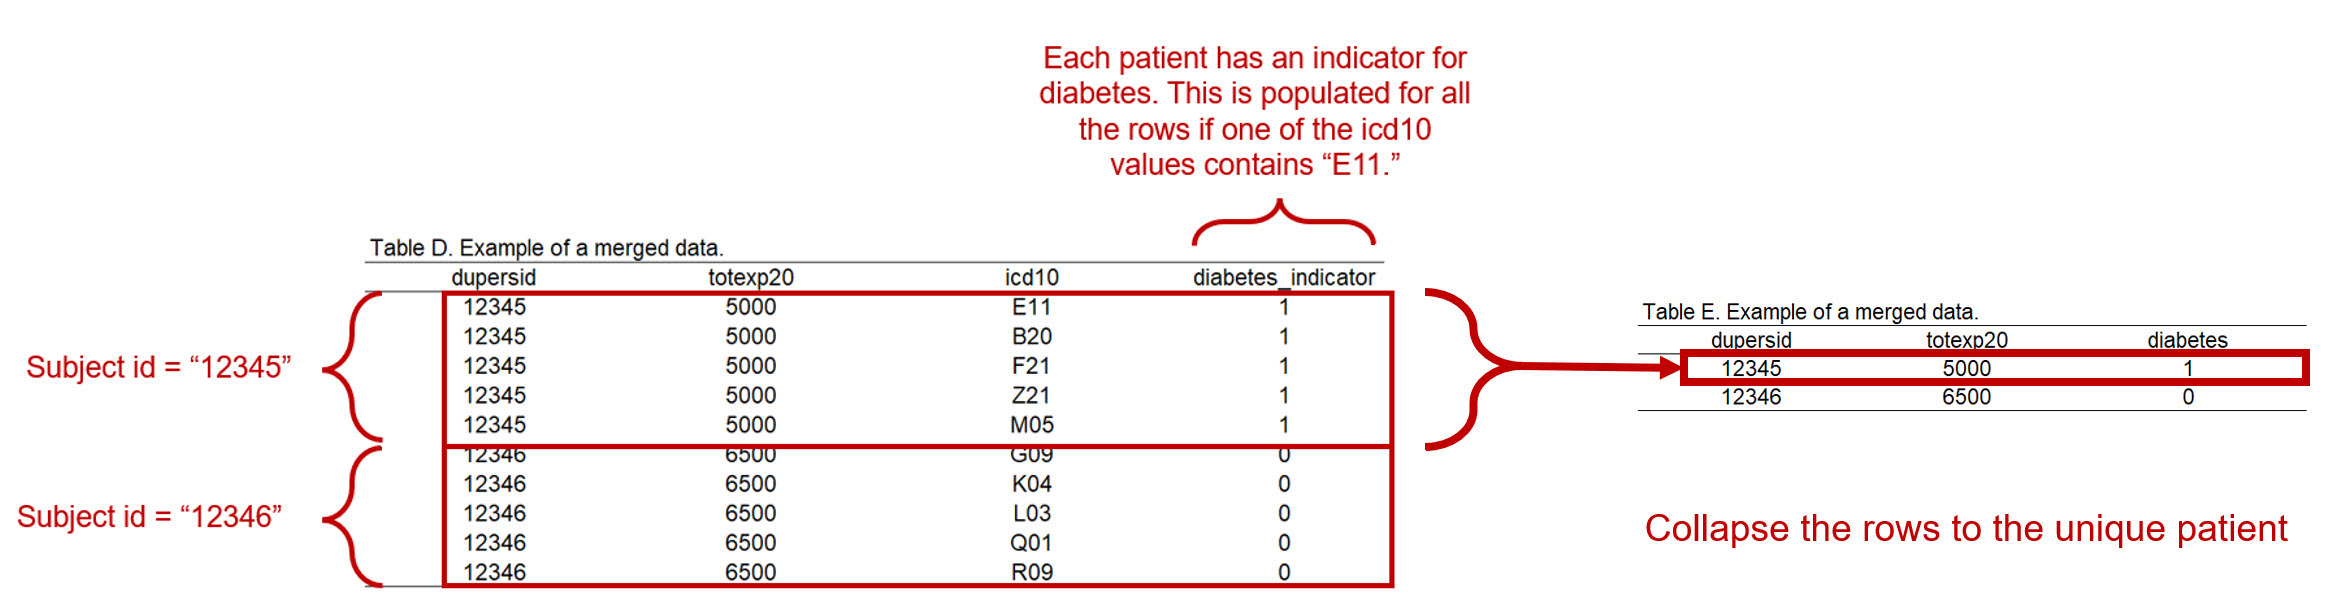
\includegraphics[width=1\linewidth]{Figure 2_6} \caption{Figure 6 - Collapse rows to a unique patient with a diabetes indicator.}\label{fig:unnamed-chunk-22}
\end{figure}

\hypertarget{conclusions-1}{%
\section{Conclusions}\label{conclusions-1}}

With this tutorial, we've learned how to merge two data files from MEPS and collapse them to a dataframe of unique patients. MEPS has additional data files that contain information that might be important for your work. For example, we can use these methods to merge the Prescription Drug file and create indicators for patients who are on opioids. However, you will need to carefully read through the documentation for each data file to understand what kind of information they contain. Feel free to explore using these strategies to merge additional MEPS data files to your existing cohort.

\hypertarget{acknowledgements-1}{%
\section{Acknowledgements}\label{acknowledgements-1}}

There are a lot of tutorials on how to use MEPS data with R. I found the \href{https://github.com/HHS-AHRQ/MEPS}{AHRQ MEPS GitHub page} to be an invaluable resource.

\href{https://daranzolin.github.io/}{David Ranzolin} has a great \href{https://rstudio-pubs-static.s3.amazonaws.com/116317_e6922e81e72e4e3f83995485ce686c14.html\#/2}{presentation} on how to use the \texttt{mutate} function in R. I liked the examples he used, and the presentation is succint and informative.

Another great resource is by \href{https://statisticsglobe.com/joachim-schork/}{Joachim Schork}, author and founder of \href{https://statisticsglobe.com/}{Statistics Globe} who wrote a great \href{https://statisticsglobe.com/sum-duplicate-rows-r}{blog} about collapsing data on a unique identifier.

I learned how to use the \texttt{left\_join} function from this \href{https://www.infoworld.com/article/3454356/how-to-merge-data-in-r-using-r-merge-dplyr-or-datatable.html}{blog} by \href{https://www.infoworld.com/author/Sharon-Machlis/}{Sharon Machlis} on \href{https://www.infoworld.com}{InfoWorld}. She uses \texttt{dplyr} to invoke the \texttt{left\_join} function which is a based on \texttt{SQL} language.

This is a work in progress, and I may update this in the future.

\hypertarget{weights}{%
\chapter{Applying weights}\label{weights}}

\hypertarget{introduction-2}{%
\section{Introduction}\label{introduction-2}}

The \href{https://www.meps.ahrq.gov/mepsweb/}{Medical Expenditure Panel Survey (MEPS)} is based on a complex survey design. Hence, it is necessary to apply survey weights to generate estimates that are representative of the United States (US) population. The weights take into account the stratification, clustering, sampling, and non-response based on the Current Population Survey. Although you can perform descriptive and complex analyses without the weights, they will not provide you with accurate standard errors of the population. Rather, not applying the weights will only yield standard errors for the sample.

\hypertarget{types-of-weights}{%
\section{Types of weights}\label{types-of-weights}}

In MEPS, there are three types of weights that are critical for most descriptive and multivariate analyses: person weight (\texttt{perwtXXf}), stratum (\texttt{varstr}), and cluster (\texttt{varpsu}). The \texttt{XX} is replaced by the year of the survey. For example, the person weight in 2020 is labelled as \texttt{perwt20f}.

\hypertarget{loading-the-data}{%
\section{Loading the data}\label{loading-the-data}}

Let's use the MEPS Full-Year Consolidated File from 2020. From our previous tutorial, you can load data using the \texttt{MEPS} library function \texttt{read\_MEPS}. There are two methods that you can use to load data into R.

\begin{Shaded}
\begin{Highlighting}[]
\DocumentationTok{\#\#\# Load the MEPS package}
\FunctionTok{library}\NormalTok{(}\StringTok{"MEPS"}\NormalTok{) }\DocumentationTok{\#\# You need to load the library every time you restart R}

\DocumentationTok{\#\#\#\# Method 1: Load data from AHRQ MEPS website}
\NormalTok{hc2020 }\OtherTok{=} \FunctionTok{read\_MEPS}\NormalTok{(}\AttributeTok{file =} \StringTok{"h224"}\NormalTok{)}

\DocumentationTok{\#\#\#\# Method 2: Load data from AHRQ MEPS website}
\NormalTok{hc2020 }\OtherTok{=} \FunctionTok{read\_MEPS}\NormalTok{(}\AttributeTok{year =} \DecValTok{2020}\NormalTok{, }\AttributeTok{type =} \StringTok{"FYC"}\NormalTok{)}

\DocumentationTok{\#\# Change column names to lowercase}
\FunctionTok{names}\NormalTok{(hc2020) }\OtherTok{\textless{}{-}} \FunctionTok{tolower}\NormalTok{(}\FunctionTok{names}\NormalTok{(hc2020))}
\end{Highlighting}
\end{Shaded}

Once the data has been loaded, we can look at how many variables there are.

\begin{Shaded}
\begin{Highlighting}[]
\DocumentationTok{\#\# The number of columns represents the number of variables in the hc2020 dataframe. }
\FunctionTok{ncol}\NormalTok{(hc2020)}
\end{Highlighting}
\end{Shaded}

\begin{verbatim}
## [1] 1451
\end{verbatim}

We have over 1400 variable. This is a very large dataframe. We can reduce this to a manageable size by keeping only the variables that are important. Let's keep the unique patient identifier (\texttt{dupersid}), weights (\texttt{perwt20f}, \texttt{varstr}, and \texttt{varpsu}), and the total expenditures (\texttt{totexp20}).

\begin{Shaded}
\begin{Highlighting}[]
\DocumentationTok{\#\# Create a smaller dataframe}
\NormalTok{keep\_hc2020 }\OtherTok{\textless{}{-}} \FunctionTok{subset}\NormalTok{(hc2020, }\AttributeTok{select =} \FunctionTok{c}\NormalTok{(dupersid, perwt20f, varstr, varpsu, totexp20, sex, povcat20))}
\FunctionTok{head}\NormalTok{(keep\_hc2020)}
\end{Highlighting}
\end{Shaded}

\begin{verbatim}
## # A tibble: 6 x 7
##   dupersid   perwt20f varstr varpsu totexp20 sex          povcat20           
##   <chr>         <dbl>  <dbl>  <dbl>    <dbl> <dbl+lbl>    <dbl+lbl>          
## 1 2320005101    8418.   2079      1      459 2 [2 FEMALE] 2 [2 NEAR POOR]    
## 2 2320005102    5200.   2079      1      564 1 [1 MALE]   2 [2 NEAR POOR]    
## 3 2320006101    2140.   2028      1      140 2 [2 FEMALE] 3 [3 LOW INCOME]   
## 4 2320006102    2216.   2028      1     4673 1 [1 MALE]   1 [1 POOR/NEGATIVE]
## 5 2320006103    4157.   2028      1      410 1 [1 MALE]   3 [3 LOW INCOME]   
## 6 2320012102    1961.   2069      2     2726 2 [2 FEMALE] 3 [3 LOW INCOME]
\end{verbatim}

We can add labels to the \texttt{sex} variable where \texttt{1\ =\ male} and \texttt{2\ =\ female}.

\hypertarget{perform-descriptive-analysis}{%
\section{Perform descriptive analysis}\label{perform-descriptive-analysis}}

Now that we have a smaller dataframe with the variables of interest, let's apply the survey weights to some descriptive analysis.

Suppose you were interested in the average age of the cohort. You will need to apply the survey weights to generate the mean and standard deviation. The \texttt{survey} package comes with the \texttt{svydesign} function, which uses the survey weights in the Full-Year Consolidated File data and applies them to the cohort in preparation for analyses.

First, you will need to set the options to \texttt{adjust}, which centers the single-PSU strata arund the grand mean rather than the stratum mean. With MEPS data, we are using single-PSU (or ``lonely'' PSU), which is used to estimate the variance by calculating the difference of the sum of the statum's PSU and the average statum's PSU. The, we use the \texttt{svydesign} function to generate a complex survey design dataset (which we will call \texttt{mepsdsgn}) for analysis by applying the survey weights.

\begin{Shaded}
\begin{Highlighting}[]
\DocumentationTok{\#\# Load the "survey" package}
\FunctionTok{library}\NormalTok{(}\StringTok{"survey"}\NormalTok{)}

\DocumentationTok{\#\# Apply the survey weights to the dataframe using the svydesign function}
\FunctionTok{options}\NormalTok{(}\AttributeTok{survey.lonely.psu =} \StringTok{\textquotesingle{}adjust\textquotesingle{}}\NormalTok{)}

\NormalTok{mepsdsgn }\OtherTok{=} \FunctionTok{svydesign}\NormalTok{(}
  \AttributeTok{id =} \SpecialCharTok{\textasciitilde{}}\NormalTok{varpsu,}
  \AttributeTok{strata =} \SpecialCharTok{\textasciitilde{}}\NormalTok{varstr,}
  \AttributeTok{weights =} \SpecialCharTok{\textasciitilde{}}\NormalTok{perwt20f,}
  \AttributeTok{data =}\NormalTok{ keep\_hc2020,}
  \AttributeTok{nest =} \ConstantTok{TRUE}\NormalTok{)}
\end{Highlighting}
\end{Shaded}

Once the survey weights have been applied, we can use the \texttt{survey} functions to perform some descriptive analysis on the \texttt{mepsdsgn} data.

First, let's see how many patients we have that is representative of the US population by sex. We use the \texttt{svytable} function to generate the weight sample for males and females. Adding these together will yield the weighted sample of the US population.

\begin{Shaded}
\begin{Highlighting}[]
\DocumentationTok{\#\# Weighted sample of the population stratified by sex}
\FunctionTok{svytable}\NormalTok{(}\SpecialCharTok{\textasciitilde{}}\NormalTok{sex, }\AttributeTok{design =}\NormalTok{ mepsdsgn)}
\end{Highlighting}
\end{Shaded}

\begin{verbatim}
## sex
##   1 - Male 2 - Female 
##  160960989  167584308
\end{verbatim}

Using the survey weights, there are 160,960,989 males and 167,584,308 females. In total, there are 328,545,297 weighted subjects in the \texttt{mepsdsgn} data.

Let's move on and estimate the average total expenditures for the total sample.

\begin{Shaded}
\begin{Highlighting}[]
\DocumentationTok{\#\# Estimate the weighted mean total expenditure for the sample}
\FunctionTok{svymean}\NormalTok{(}\SpecialCharTok{\textasciitilde{}}\NormalTok{totexp20, }\AttributeTok{design =}\NormalTok{ mepsdsgn)}
\end{Highlighting}
\end{Shaded}

\begin{verbatim}
##            mean     SE
## totexp20 6266.1 164.38
\end{verbatim}

The \texttt{svymean} function generates the appropriate average and standard error (SE) of the total sample that is representative of the US population. In 2020, the average total expenditure was \$6266 (SE, 164).

In our \texttt{mepsdsgn} data, we have sex, which is a binary variable. Let's estimate the total expenditures between males and females in the MEPS Full-Year Consolidated data. To estimate the mean between two groups, we'll need to use the \texttt{svyby} function along with the \texttt{svymean} function.

\begin{Shaded}
\begin{Highlighting}[]
\DocumentationTok{\#\# Estimate the weight mean total expenditure for males and females}
\FunctionTok{svyby}\NormalTok{(}\SpecialCharTok{\textasciitilde{}}\NormalTok{totexp20, }\SpecialCharTok{\textasciitilde{}}\NormalTok{sex, mepsdsgn, svymean)}
\end{Highlighting}
\end{Shaded}

\begin{verbatim}
##                   sex totexp20       se
## 1 - Male     1 - Male 5861.278 243.5624
## 2 - Female 2 - Female 6654.998 205.0776
\end{verbatim}

The average total expenditures for male and female are \$5861 (SE, 244) and \$6655 (SE 205), respectively.

We can perform crosstabulations with the \texttt{svytable} function. Let's look at the distribution of males and females across various poverty categories. In the MEPS codebook, poverty category are groups as: 1 = Poor/Negative, 2 = Near Poor, 3 = Low Income, 4 = Middle Income, and 5 = High Income.

\begin{Shaded}
\begin{Highlighting}[]
\DocumentationTok{\#\# Crosstab sex and poverty category}
\FunctionTok{svytable}\NormalTok{(}\SpecialCharTok{\textasciitilde{}}\NormalTok{sex }\SpecialCharTok{+}\NormalTok{ povcat20, }\AttributeTok{design =}\NormalTok{ mepsdsgn)}
\end{Highlighting}
\end{Shaded}

\begin{verbatim}
##             povcat20
## sex                 1        2        3        4        5
##   1 - Male   16644995  5955576 18910001 45083571 74366846
##   2 - Female 21002826  6672752 21753502 47750327 70404901
\end{verbatim}

To generate the proportions, you will need to use \texttt{prop.table}. We add the \texttt{margin\ =\ 1} option to calculate the column total.

\begin{Shaded}
\begin{Highlighting}[]
\FunctionTok{prop.table}\NormalTok{(}\FunctionTok{svytable}\NormalTok{(}\SpecialCharTok{\textasciitilde{}}\NormalTok{sex }\SpecialCharTok{+}\NormalTok{ povcat20, }\AttributeTok{design =}\NormalTok{ mepsdsgn), }\AttributeTok{margin =} \DecValTok{1}\NormalTok{) }\DocumentationTok{\#\#\# margin = 1 calculates the column total.}
\end{Highlighting}
\end{Shaded}

\begin{verbatim}
##             povcat20
## sex                   1          2          3          4          5
##   1 - Male   0.10341012 0.03700012 0.11748189 0.28009005 0.46201783
##   2 - Female 0.12532693 0.03981729 0.12980632 0.28493316 0.42011631
\end{verbatim}

We can combine these into a contingency table using the \texttt{tbl\_svysummary} function from the \texttt{gtsummary} package. We will also use the \texttt{tidyverse} package to manipulate the data more easily.

\begin{Shaded}
\begin{Highlighting}[]
\DocumentationTok{\#\# Load libraries }
\FunctionTok{library}\NormalTok{(}\StringTok{"tidyverse"}\NormalTok{)}
\FunctionTok{library}\NormalTok{(}\StringTok{"gtsummary"}\NormalTok{)}

\DocumentationTok{\#\# Contingency table (crosstabulations between sex and poverty category)}
\NormalTok{mepsdsgn }\SpecialCharTok{\%\textgreater{}\%}
  \FunctionTok{tbl\_svysummary}\NormalTok{(}\AttributeTok{by =}\NormalTok{ sex, }\AttributeTok{percent =} \StringTok{"column"}\NormalTok{, }\AttributeTok{include =} \FunctionTok{c}\NormalTok{(povcat20))}
\end{Highlighting}
\end{Shaded}

\begin{tabular}{l|c|c}
\hline
**Characteristic** & **1 - Male**, N = 160,960,989 & **2 - Female**, N = 167,584,308\\
\hline
FAMILY INC AS \% OF POVERTY LINE - CATEGORICAL &  & \\
\hline
1 & 16,644,995 (10\%) & 21,002,826 (13\%)\\
\hline
2 & 5,955,576 (3.7\%) & 6,672,752 (4.0\%)\\
\hline
3 & 18,910,001 (12\%) & 21,753,502 (13\%)\\
\hline
4 & 45,083,571 (28\%) & 47,750,327 (28\%)\\
\hline
5 & 74,366,846 (46\%) & 70,404,901 (42\%)\\
\hline
\end{tabular}

Based on these weighted sample numbers, there are more males who are in the High Income category compared to females (46\% versus 42\%).

\hypertarget{conclusions-2}{%
\section{Conclusions}\label{conclusions-2}}

The MEPS data uses weights to generate estimations that are reflective of the US population. The \texttt{survey} package from R will allow us to apply these weights using the \texttt{svydesign} function, which requires us to enter the patient weight, stratum, and cluster values. Once these are applied, we can use the suite of functions from the \texttt{survey} package to perform descriptive analysis on the population. The \texttt{svymean} generates the population average and the \texttt{svytable} generates the population frequencies. Having a good understanding of how these weights are used with MEPS data will allow you to generate estimates of the population in your epidemiology work.

\hypertarget{acknowledgements-2}{%
\section{Acknowledgements}\label{acknowledgements-2}}

The \texttt{survey} package and functions were developed by \href{https://profiles.auckland.ac.nz/t-lumley}{Thomas Lumley} and can be found \href{https://www.rdocumentation.org/packages/survey/versions/4.1-1}{here}.

The \texttt{gtsummary} package and instructions are developed by Daniel D. Sjoberg, Joseph Larmarange, Michael Curry, Jessica Lavery, Karissa Whiting, Emily C. Zabor, which can be found at their \href{https://www.danieldsjoberg.com/gtsummary/reference/tbl_svysummary.html}{website}.

This is a work in progress, and I expect to make updates in the future.

\hypertarget{clnk}{%
\chapter{\texorpdfstring{Using condition-event link (\texttt{CLNK}) file}{Using condition-event link (CLNK) file}}\label{clnk}}

\hypertarget{introduction-3}{%
\section{Introduction}\label{introduction-3}}

The Agency for Healthcare Research and Quality (AHRQ) Medical Expenditure Panel Survey (MEPS) categorizes expenditures into different components. Healthcare expenditures (e.g., costs and utilization) are provided for each individual respondent in MEPS. For instance, healthcare expenditures are categorized as total healthcare expenditures (\texttt{totexp21}), office-based expenditures (\texttt{obvexp21}), outpatient expenditures (\texttt{opvexp21}), inpatient expenditures (\texttt{iptexp21}), and prescription expenditures (\texttt{rxexp21}) to name a few. Reading the long but detailed \href{https://meps.ahrq.gov/data_stats/download_data/pufs/h233/h233doc.shtml}{documentation} is a good way to learn more about the different expenditure categories. Moreover, you can also review \textbf{Appendix 3} of the documentation (see Figure below).

\begin{figure}
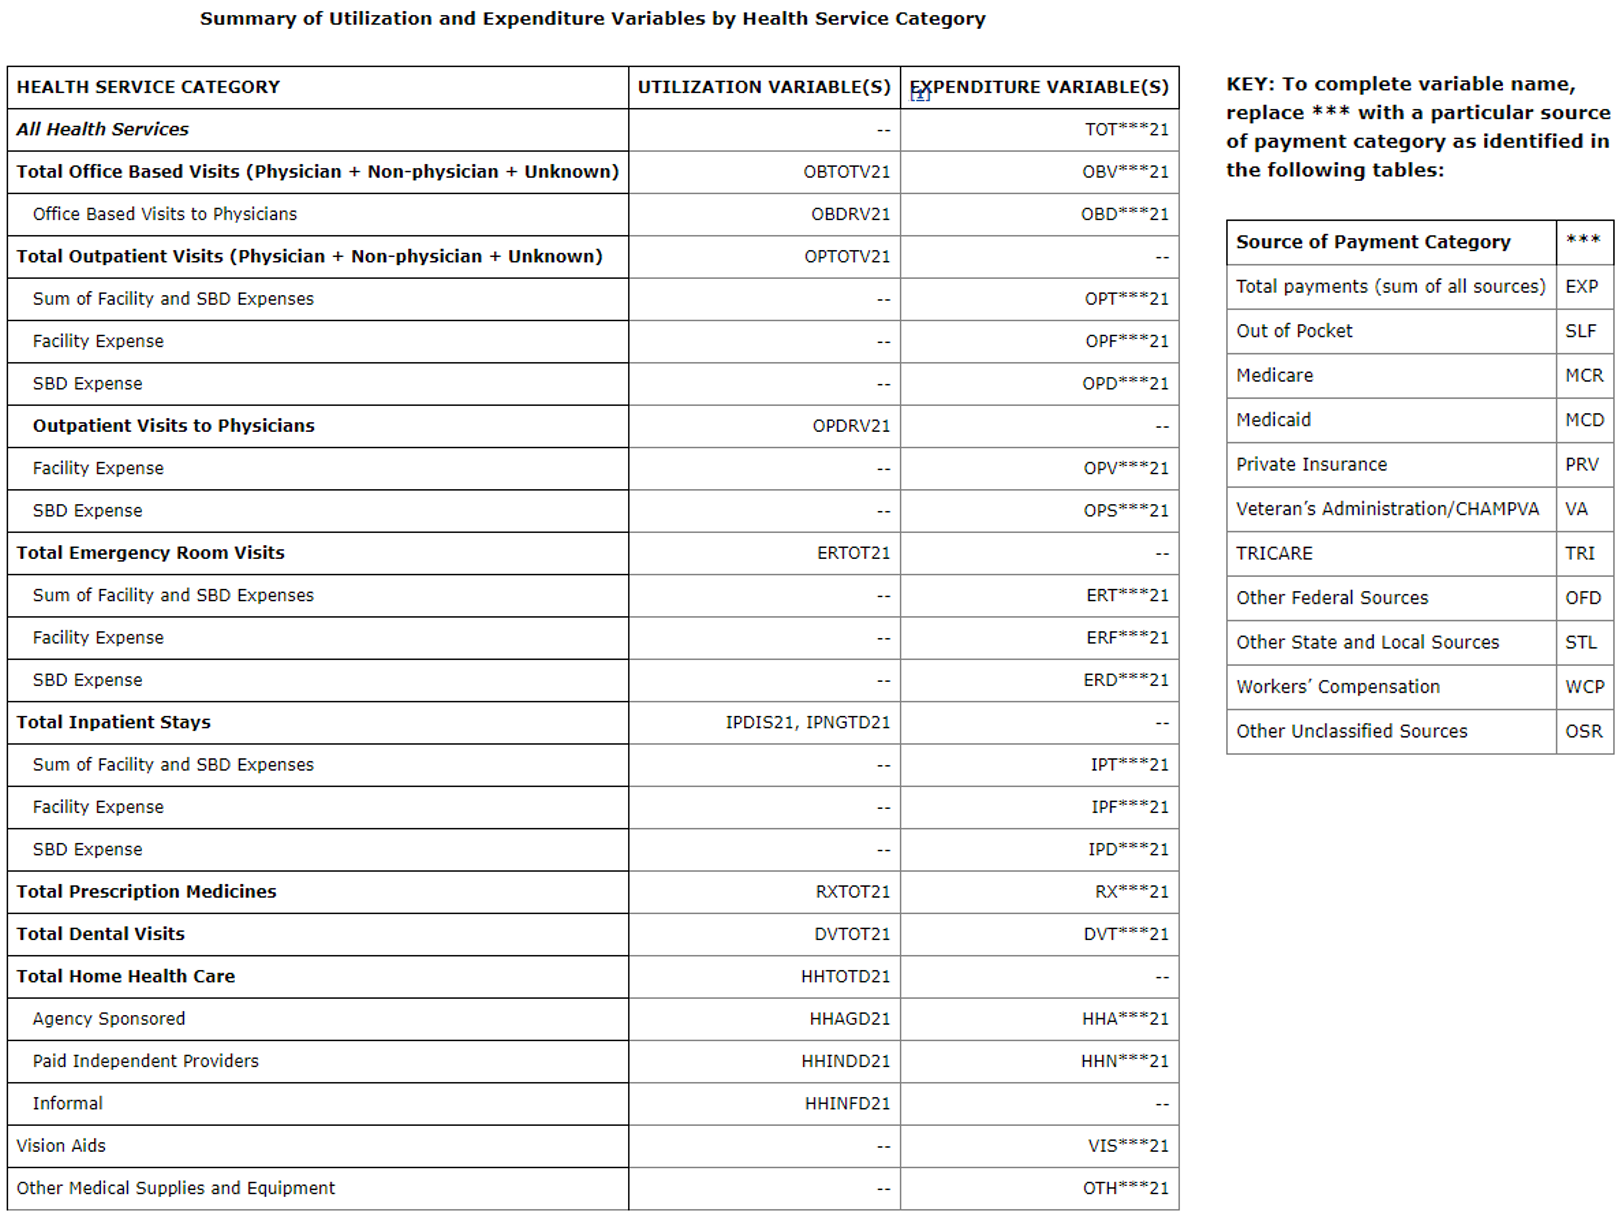
\includegraphics[width=1\linewidth]{Figure 4_1 - Appendix 3} \caption{MEPS Appendix 3 - Expenditure variables}\label{fig:unnamed-chunk-34}
\end{figure}

These costs and utilization provide information about the annual expenditures associated with each category for each individual respondent. But this doesn't provide disease-specific expenditures. For example, an individual may have an annual office-based visits healthcare cost of \$10,000, but part of this costs may be due to a specific disease such as migraine. How much of the \$10,000 is due to migraine-related office-based visits? One can answer this question using the \href{https://meps.ahrq.gov/data_stats/download_data/pufs/h229i/h229idoc.shtml}{condition-event link (\texttt{CLNK}) file}.

The \texttt{CLNK} file has a unique variable that can be used to link each record on the \href{https://meps.ahrq.gov/data_stats/download_data_files_detail.jsp?cboPufNumber=HC-231}{Medical Conditions file} with event files from the respective year (e.g., \texttt{HC-229D} through \texttt{HC-229H}). One of these event files that we're interested in is the office-based event file (\texttt{HC-229G}). The \texttt{CLNK} file contains 6 variables:

\begin{itemize}
\item
  \texttt{dupersid} - 10-digit unique identifier
\item
  \texttt{condidx} - 13-digit unique identifier for a condition
\item
  \texttt{evntidx} - 16-digit unique identifier for each event
\item
  \texttt{clnkidx} - 29-digit unique identifier for each record; combines \texttt{condidx} and \texttt{evntidx}
\item
  \texttt{eventype} - indicates the type of event record (see Figure)
\item
  \texttt{panel} - indicate the panel when the interview occurred
\end{itemize}

\begin{figure}
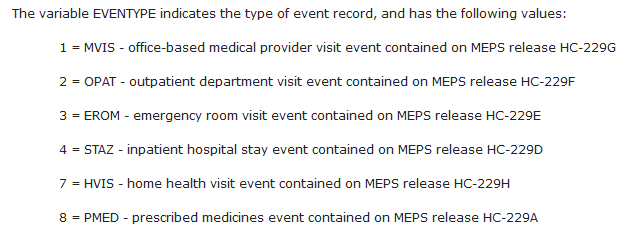
\includegraphics[width=1\linewidth]{Figure 4_2} \caption{Type of event record (`eventype`)}\label{fig:unnamed-chunk-35}
\end{figure}

Using these files, we can acquire disease-specific expenditures from MEPS data, which may be important for those of us who are interested in these expenditures.

\hypertarget{motivating-example---migraine-specific-expenditures}{%
\section{Motivating example - Migraine-specific expenditures}\label{motivating-example---migraine-specific-expenditures}}

In this motivating example, we will review how to use MEPS to find the office-based expenditures and inpatient expenditures specific to migraine.

\hypertarget{part-1---setup}{%
\subsection{Part 1 - Setup}\label{part-1---setup}}

We will need to install several packages. The \href{https://github.com/HHS-AHRQ/MEPS}{AHRQ MEPS GitHub site} is a great source for documents, tutorials, codes, and updates. I learned a ton going through their exercises, and a lot of the code you'll see in this tutorial come from those resources.

\begin{Shaded}
\begin{Highlighting}[]
\CommentTok{\# To install "MEPS" package in R, you need to do a couple of things.}
\DocumentationTok{\#\#\# Step 1: Install the "devtools" package. }
\CommentTok{\#install.packages("devtools")}


\DocumentationTok{\#\#\# Step 2: Install the "MEPS" package from the AHRQ MEPS GitHub site. }
\CommentTok{\#devtools::install\_github("e{-}mitchell/meps\_r\_pkg/MEPS")}


\DocumentationTok{\#\#\# Step 3: Load the MEPS package}
\FunctionTok{library}\NormalTok{(}\StringTok{"MEPS"}\NormalTok{) }\DocumentationTok{\#\# You need to load the library every time you restart R}

\DocumentationTok{\#\#\# Step 4: Load the other libraries}
\FunctionTok{library}\NormalTok{(}\StringTok{"survey"}\NormalTok{)}
\FunctionTok{library}\NormalTok{(}\StringTok{"foreign"}\NormalTok{)}
\FunctionTok{library}\NormalTok{(}\StringTok{"tidyverse"}\NormalTok{)}
\FunctionTok{library}\NormalTok{(}\StringTok{"psych"}\NormalTok{)}
\end{Highlighting}
\end{Shaded}

Next, we set the global options.

\begin{Shaded}
\begin{Highlighting}[]
\CommentTok{\# Set global options}
\FunctionTok{options}\NormalTok{(}\AttributeTok{survey.lonely.psu =} \StringTok{"adjust"}\NormalTok{) }\CommentTok{\# survey option for lonely PSUs}
\FunctionTok{options}\NormalTok{(}\AttributeTok{dplyr.width =} \ConstantTok{Inf}\NormalTok{) }\CommentTok{\# Columns are not truncated}
\FunctionTok{options}\NormalTok{(}\AttributeTok{digits =} \DecValTok{10}\NormalTok{) }\CommentTok{\# Do not use scientific notation for large number}
\end{Highlighting}
\end{Shaded}

Once that's done, we will download the data directly from the MEPS site using the \texttt{read\_MEPS} function. There are two ways to do this:

\begin{Shaded}
\begin{Highlighting}[]
\CommentTok{\# There are two ways to load data from AHRQ MEPS website:}
\DocumentationTok{\#\#\#\# Method 1: Load data from AHRQ MEPS website}
\NormalTok{hc2021 }\OtherTok{=} \FunctionTok{read\_MEPS}\NormalTok{(}\AttributeTok{file =} \StringTok{"h233"}\NormalTok{) }\CommentTok{\# Full{-}year consolidated file}
\NormalTok{ob2021 }\OtherTok{=} \FunctionTok{read\_MEPS}\NormalTok{(}\AttributeTok{file =} \StringTok{"h229g"}\NormalTok{) }\CommentTok{\# Office{-}based visits}
\NormalTok{inpat2021 }\OtherTok{=} \FunctionTok{read\_MEPS}\NormalTok{(}\AttributeTok{file =} \StringTok{"h229d"}\NormalTok{) }\CommentTok{\# Inpatient stays}
\NormalTok{cond2021 }\OtherTok{=} \FunctionTok{read\_MEPS}\NormalTok{(}\AttributeTok{file =} \StringTok{"h231"}\NormalTok{) }\CommentTok{\# Medical conditions file}
\NormalTok{clnk2021 }\OtherTok{=} \FunctionTok{read\_MEPS}\NormalTok{(}\AttributeTok{file =} \StringTok{"h229IF1"}\NormalTok{) }\CommentTok{\# Condition{-}Event Link File (CLNK)}


\DocumentationTok{\#\#\#\# Method 2: Load data from AHRQ MEPS website}
\NormalTok{hc2021 }\OtherTok{=} \FunctionTok{read\_MEPS}\NormalTok{(}\AttributeTok{year =} \DecValTok{2021}\NormalTok{, }\AttributeTok{type =} \StringTok{"FYC"}\NormalTok{) }\CommentTok{\# Full{-}year consolidated file}
\NormalTok{ob2021 }\OtherTok{=} \FunctionTok{read\_MEPS}\NormalTok{(}\AttributeTok{year =} \DecValTok{2021}\NormalTok{, }\AttributeTok{type =} \StringTok{"OB"}\NormalTok{) }\CommentTok{\# Office{-}based visits}
\NormalTok{inpat2021 }\OtherTok{=} \FunctionTok{read\_MEPS}\NormalTok{(}\AttributeTok{year =} \DecValTok{2021}\NormalTok{, }\AttributeTok{type =} \StringTok{"IP"}\NormalTok{) }\CommentTok{\# Inpatient stays}
\NormalTok{cond2021 }\OtherTok{=} \FunctionTok{read\_MEPS}\NormalTok{(}\AttributeTok{year =} \DecValTok{2021}\NormalTok{, }\AttributeTok{type =} \StringTok{"COND"}\NormalTok{) }\CommentTok{\# Medical conditions file}
\NormalTok{clnk2021 }\OtherTok{=} \FunctionTok{read\_MEPS}\NormalTok{(}\AttributeTok{year =} \DecValTok{2021}\NormalTok{, }\AttributeTok{type =} \StringTok{"CLNK"}\NormalTok{) }\CommentTok{\# Condition{-}Event Link File (CLNK)}
\end{Highlighting}
\end{Shaded}

After the data are loaded, you can change the column names from upper case to lower case.

\begin{Shaded}
\begin{Highlighting}[]
\DocumentationTok{\#\# Change column names to lowercase}
\FunctionTok{names}\NormalTok{(hc2021) }\OtherTok{\textless{}{-}} \FunctionTok{tolower}\NormalTok{(}\FunctionTok{names}\NormalTok{(hc2021))}
\FunctionTok{names}\NormalTok{(ob2021) }\OtherTok{\textless{}{-}} \FunctionTok{tolower}\NormalTok{(}\FunctionTok{names}\NormalTok{(ob2021))}
\FunctionTok{names}\NormalTok{(inpat2021) }\OtherTok{\textless{}{-}} \FunctionTok{tolower}\NormalTok{(}\FunctionTok{names}\NormalTok{(inpat2021))}
\FunctionTok{names}\NormalTok{(cond2021) }\OtherTok{\textless{}{-}} \FunctionTok{tolower}\NormalTok{(}\FunctionTok{names}\NormalTok{(cond2021))}
\FunctionTok{names}\NormalTok{(clnk2021) }\OtherTok{\textless{}{-}} \FunctionTok{tolower}\NormalTok{(}\FunctionTok{names}\NormalTok{(clnk2021))}
\end{Highlighting}
\end{Shaded}

Each of these tables will have a lot of variables. To make things easier and cleaner, let's reduce the size of the tables to only include the essential variables.

\begin{Shaded}
\begin{Highlighting}[]
\CommentTok{\# Keep only the variables of interest}
\NormalTok{hc2021x }\OtherTok{=}\NormalTok{ hc2021 }\SpecialCharTok{\%\textgreater{}\%}
  \FunctionTok{select}\NormalTok{(dupersid, totexp21, obvexp21, iptexp21, perwt21f, varpsu, varstr, sex, racev1x)}

\NormalTok{ob2021x }\OtherTok{=}\NormalTok{ ob2021 }\SpecialCharTok{\%\textgreater{}\%}
  \FunctionTok{select}\NormalTok{(dupersid, evntidx, eventrn, obdateyr, obdatemm, obxp21x, perwt21f, varpsu, varstr)}

\NormalTok{inpat2021x }\OtherTok{=}\NormalTok{ inpat2021 }\SpecialCharTok{\%\textgreater{}\%}
  \FunctionTok{select}\NormalTok{(dupersid, evntidx, eventrn, numnighx, ipxp21x, perwt21f, varpsu, varstr)}

\NormalTok{cond2021x }\OtherTok{=}\NormalTok{ cond2021 }\SpecialCharTok{\%\textgreater{}\%}
  \FunctionTok{select}\NormalTok{(dupersid, condidx, icd10cdx, ccsr1x}\SpecialCharTok{:}\NormalTok{ccsr3x)}
\end{Highlighting}
\end{Shaded}

Next, we want identify migraine condition from the \texttt{cond2021x} file, which is the medical conditions file. The CCSR code for migraine is \texttt{NVS010} (note: the ICD10 code for migraine is \texttt{G42}, but we won't need it for this example). There are three CCSR columns (\texttt{ccsr1x}, \texttt{ccsr2x}, \texttt{ccsr3x}), and we want to concatenate these into a new column called \texttt{all\_CCSR} to isolate for migraine. You can find the list of CCSR codes in the \href{https://github.com/HHS-AHRQ/MEPS/blob/master/Quick_Reference_Guides/meps_ccsr_conditions.csv}{AHRQ MEPS site}.

\begin{Shaded}
\begin{Highlighting}[]
\DocumentationTok{\#\#\#\#\#\#\#\#\#\#\#\#\#\#\#\#\#\#\#\#\#\#\#\#\#\#\#\#\#\#\#\#\# NOTES \#\#\#\#\#\#\#\#\#\#\#\#\#\#\#\#\#\#\#\#\#\#\#\#\#\#\#\#\#\#\#\#\# }
\DocumentationTok{\#\# Use CLNK file to map condition with events}
\DocumentationTok{\#\# CCSR code: https://github.com/HHS{-}AHRQ/MEPS/blob/master/Quick\_Reference\_Guides/meps\_ccsr\_conditions.csv}
\DocumentationTok{\#\# CCSR code for migraine: NVS010}
\DocumentationTok{\#\# ICD10 code for migraine: G43}
\DocumentationTok{\#\#\#\#\#\#\#\#\#\#\#\#\#\#\#\#\#\#\#\#\#\#\#\#\#\#\#\#\#\#\#\#\#\#\#\#\#\#\#\#\#\#\#\#\#\#\#\#\#\#\#\#\#\#\#\#\#\#\#\#\#\#\#\#\#\#\#\#\#\#\#\#\# }

\CommentTok{\# Restrict conditions to Migraine only from the conditions file}
\DocumentationTok{\#\#\# This creates a variable called "all\_CCSR" which concatenates the CCSR columns}
\DocumentationTok{\#\#\# Then, filter() only selects rows with the "NVS010" text in the "all\_CCSR" column}
\DocumentationTok{\#\#\# Finally, this gets saved into the "migraine" object.}
\NormalTok{migraine }\OtherTok{=}\NormalTok{ cond2021x }\SpecialCharTok{\%\textgreater{}\%} 
  \FunctionTok{unite}\NormalTok{(}\StringTok{"all\_CCSR"}\NormalTok{, ccsr1x}\SpecialCharTok{:}\NormalTok{ccsr3x, }\AttributeTok{remove =} \ConstantTok{FALSE}\NormalTok{) }\SpecialCharTok{\%\textgreater{}\%} 
  \FunctionTok{filter}\NormalTok{(}\FunctionTok{grepl}\NormalTok{(}\StringTok{"NVS010"}\NormalTok{, all\_CCSR))}


\CommentTok{\# View freq per diagnosis code type (Pretty nice code from AHRQ)}
\NormalTok{migraine }\SpecialCharTok{\%\textgreater{}\%} 
  \FunctionTok{count}\NormalTok{(icd10cdx, ccsr1x, ccsr2x, ccsr3x) }
\end{Highlighting}
\end{Shaded}

\begin{verbatim}
## # A tibble: 3 x 5
##   icd10cdx ccsr1x ccsr2x ccsr3x     n
##   <chr>    <chr>  <chr>  <chr>  <int>
## 1 -15      NVS010 -1     -1        26
## 2 G43      NVS010 -1     -1       556
## 3 R51      NVS010 SYM010 -1       202
\end{verbatim}

\hypertarget{part-2---migraine-specific-office-based-expenditures}{%
\subsection{Part 2 - Migraine-specific office-based expenditures}\label{part-2---migraine-specific-office-based-expenditures}}

Now that we have our data files set up and prepared, we can begin to identify the migraine-specific office-based expenditures.

First, we want to isolate the office-based visits events from the \texttt{clnk2021} file. According to the figure above, \texttt{eventype\ ==\ 1} is for office-based medical provider visit event. We will save these results into a new object called \texttt{ob\_events}.

\begin{Shaded}
\begin{Highlighting}[]
\DocumentationTok{\#\#\#\#\#\#\#\#\#\#\#\#\#\#\#\#\#\#\#\#\#\#\#\#\#\#\#\#\#\#\#\#\#\#\#\#\#\#\#\#\#\#\#\#}
\DocumentationTok{\#\# OUTPATIENT VISITS}
\DocumentationTok{\#\#\#\#\#\#\#\#\#\#\#\#\#\#\#\#\#\#\#\#\#\#\#\#\#\#\#\#\#\#\#\#\#\#\#\#\#\#\#\#\#\#\#\#}
\CommentTok{\# Select Office{-}based events from the CLNK file}
\NormalTok{ob\_events }\OtherTok{=}\NormalTok{ clnk2021 }\SpecialCharTok{\%\textgreater{}\%}
  \FunctionTok{filter}\NormalTok{(eventype }\SpecialCharTok{==} \DecValTok{1}\NormalTok{)}
\end{Highlighting}
\end{Shaded}

Next, we want to merge the \texttt{ob\_events} object with the \texttt{migraine} object, which contains the migraine-related conditions. We use an \texttt{inner\_join}, which will only subset rows that matches between the two objects by \texttt{dupersid} and \texttt{condidx}. This will be saved as a new object called \texttt{migraine\_lnk}.

\begin{Shaded}
\begin{Highlighting}[]
\CommentTok{\# Merge migraine diagnosis conditions file with office{-}based visit file}
\NormalTok{migraine\_lnk }\OtherTok{=} \FunctionTok{inner\_join}\NormalTok{(}
\NormalTok{  migraine, ob\_events,}
  \AttributeTok{by =} \FunctionTok{c}\NormalTok{(}\StringTok{"dupersid"}\NormalTok{, }\StringTok{"condidx"}\NormalTok{)}
\NormalTok{)}
\end{Highlighting}
\end{Shaded}

Since the \texttt{migraine\_lnk} object has duplicate \texttt{dupersid} and \texttt{condidx}, we want to create an updated dataframe (\texttt{migraine\_ob\_distinct}) that contains unique rows of \texttt{dupersid}, \texttt{evntidx}, and \texttt{eventype}. AHRQ called this process ``De-duplicate.'' We will use this term in our exercise.

\begin{Shaded}
\begin{Highlighting}[]
\CommentTok{\# Select only DISTINCT office{-}based events ("De{-}duplicate")}
\NormalTok{migraine\_ob\_distinct }\OtherTok{=}\NormalTok{ migraine\_lnk }\SpecialCharTok{\%\textgreater{}\%}
  \FunctionTok{distinct}\NormalTok{(dupersid, evntidx, eventype)}
\end{Highlighting}
\end{Shaded}

Then we merge the \texttt{migraine\_ob\_distinct} dataframe with the \texttt{ob2021x} dataframe using the \texttt{inner\_join} function because we want to only include the rows that are in both dataframes. We use the \texttt{mutate} function to generate a new indicator variable called \texttt{migrane\_ob\_visit\ =1}. This will yield a dataframe that contains the office-based events specific for migraines.

\begin{Shaded}
\begin{Highlighting}[]
\CommentTok{\# Merge office{-}based file with distinct office{-}based CLNK event file}
\DocumentationTok{\#\#\# Use the inner\_join() to merge ob2021x and migraine\_lnk\_distinct dataframes}
\DocumentationTok{\#\#\# Then create a new indicator variable called "migraine\_ob\_visit = 1."}
\NormalTok{ob\_migraine }\OtherTok{=} \FunctionTok{inner\_join}\NormalTok{(}
\NormalTok{  ob2021x, migraine\_ob\_distinct) }\SpecialCharTok{\%\textgreater{}\%}
  \FunctionTok{mutate}\NormalTok{(}\AttributeTok{migraine\_ob\_visit =} \DecValTok{1}\NormalTok{)}
\end{Highlighting}
\end{Shaded}

Once that's done, we can merge the \texttt{ob\_migraine} dataframe with the Full-Year Consolidated (\texttt{hc2021x}) dataframe. We create two indiciator variables: \texttt{migraine\_ob\ =\ 1} to capture the total number of migraine-specific office-based visits, and \texttt{fyc\ =\ 1} to indicate that this is the Full-Year Consolidated file that was merged.

\begin{Shaded}
\begin{Highlighting}[]
\CommentTok{\# Merge with full{-}year consolidated file}
\DocumentationTok{\#\#\# Use the full\_join() to keep all the rows from both dataframes.}
\DocumentationTok{\#\#\# Then create a new object called hc2021\_ob\_migraine}
\DocumentationTok{\#\#\# \& a new indicator variable called "migraine\_ob = 1"}
\DocumentationTok{\#\#\# \& another new indicator variable called "fyc = 1."}
\DocumentationTok{\#\#\# Note: These are not unique rows (repeated dupersid)}
\NormalTok{hc2021\_ob\_migraine }\OtherTok{=} \FunctionTok{full\_join}\NormalTok{(}
\NormalTok{  ob\_migraine }\SpecialCharTok{\%\textgreater{}\%} \FunctionTok{mutate}\NormalTok{(}\AttributeTok{migraine\_ob =} \DecValTok{1}\NormalTok{),}
\NormalTok{  hc2021x }\SpecialCharTok{\%\textgreater{}\%} \FunctionTok{mutate}\NormalTok{(}\AttributeTok{fyc =} \DecValTok{1}\NormalTok{))}
\end{Highlighting}
\end{Shaded}

Since this dataframe (\texttt{hc2021\_ob\_migraine}) contains duplicate \texttt{dupersid}, we want to create a dataframe where each row reflects a unique \texttt{dupersid}. We can do this by using the \texttt{group\_by} function on specific variables that we know are unique to an individual (\texttt{dupersid}, \texttt{varstr}, \texttt{varpsu}, and \texttt{perwt21f}). These are the unique identifier of the individual and their associated stratum and weight.

We also will summarize the migraine-specific utilization such as office-based visit costs (\texttt{obxp21x}) and the total sum of those visits (\texttt{migraine\_ob\_visit}).

\begin{Shaded}
\begin{Highlighting}[]
\CommentTok{\# Aggregate to person{-}level}
\DocumentationTok{\#\#\# We have to do the estimations for the person{-}level at this stage}
\DocumentationTok{\#\#\# We will estimate the total and mean values of the migraine{-}related expenditures}
\DocumentationTok{\#\#\# The "migraine\_ob" will be used to create an indicator for migraine{-}related expenditures}
\DocumentationTok{\#\#\# Need to set NA {-}\textgreater{} zero.}
\NormalTok{per\_migraine\_ob }\OtherTok{=}\NormalTok{ hc2021\_ob\_migraine }\SpecialCharTok{\%\textgreater{}\%}
  \FunctionTok{group\_by}\NormalTok{(dupersid, varstr, varpsu, perwt21f) }\SpecialCharTok{\%\textgreater{}\%}
  \FunctionTok{summarize}\NormalTok{(}
    \AttributeTok{avgtotexp\_tot               =} \FunctionTok{mean}\NormalTok{(totexp21),  }\CommentTok{\# average total expenditure}
    \AttributeTok{totexp\_ob                   =} \FunctionTok{sum}\NormalTok{(obxp21x),    }\CommentTok{\# sum of migraine{-}specific office{-}based visits per person}
    \AttributeTok{avgexp\_obvexp               =} \FunctionTok{mean}\NormalTok{(obvexp21),  }\CommentTok{\# average office{-}based visits per person}
    \AttributeTok{totvisit\_ob                 =} \FunctionTok{sum}\NormalTok{(migraine\_ob\_visit), }\CommentTok{\# sum of migraine{-}specific office{-}based visits}
    \AttributeTok{avgvisit\_migraine\_ob        =} \FunctionTok{mean}\NormalTok{(migraine\_ob\_visit), }\CommentTok{\# average migraine{-}specific office{-}based visits}
    \AttributeTok{avgvisit\_migraine\_visits\_ob =} \FunctionTok{mean}\NormalTok{(migraine\_ob), }\CommentTok{\# average migraine{-}specific office{-}based visits}
    \AttributeTok{migraine\_ob                 =} \FunctionTok{max}\NormalTok{(migraine\_ob)) }\SpecialCharTok{\%\textgreater{}\%} \CommentTok{\# indicator for migraine{-}specific expenditures}
    \FunctionTok{replace\_na}\NormalTok{(}
      \FunctionTok{list}\NormalTok{(}\AttributeTok{totexp\_ob =} \DecValTok{0}\NormalTok{, }\AttributeTok{totvisit\_ob =} \DecValTok{0}\NormalTok{, }\AttributeTok{totvisit\_migraine\_ob =} \DecValTok{0}\NormalTok{, }\AttributeTok{avgvisit\_migraine\_ob =} \DecValTok{0}\NormalTok{, }\AttributeTok{avgvisit\_migraine\_visits\_ob =} \DecValTok{0}\NormalTok{, }\AttributeTok{migraine\_ob =} \DecValTok{0}\NormalTok{)}
\NormalTok{    )}
\end{Highlighting}
\end{Shaded}

The above code chunk seems intimidating, but there are sensible reasons why it is written this way. See the Figure below for a visual explanation.

The migraine-specific office-based costs and visits are expenditures that are at the event level denoted by the event identifier \texttt{evntidx}. Costs like the total expenditures and office-based costs are at the individual level denoted by the individual identifier \texttt{dupersid}. Hence, you will see that at the event level, the migraine-specific office-based costs \texttt{obxp21x} differs by events (\texttt{evntidx}. Conversely, the office-based costs are the same by individual (\texttt{dupersid}).

We need to sum or add up the migraine-specific office-based costs for each individual so that we can collapse the rows. We want to do create a new dataframe where each row is a unique individual denoted by their individual identifier (\texttt{dupersid}) and corresponding survey weights (\texttt{varstr}, \texttt{varpsu}, \texttt{perwt21f}).

\begin{figure}
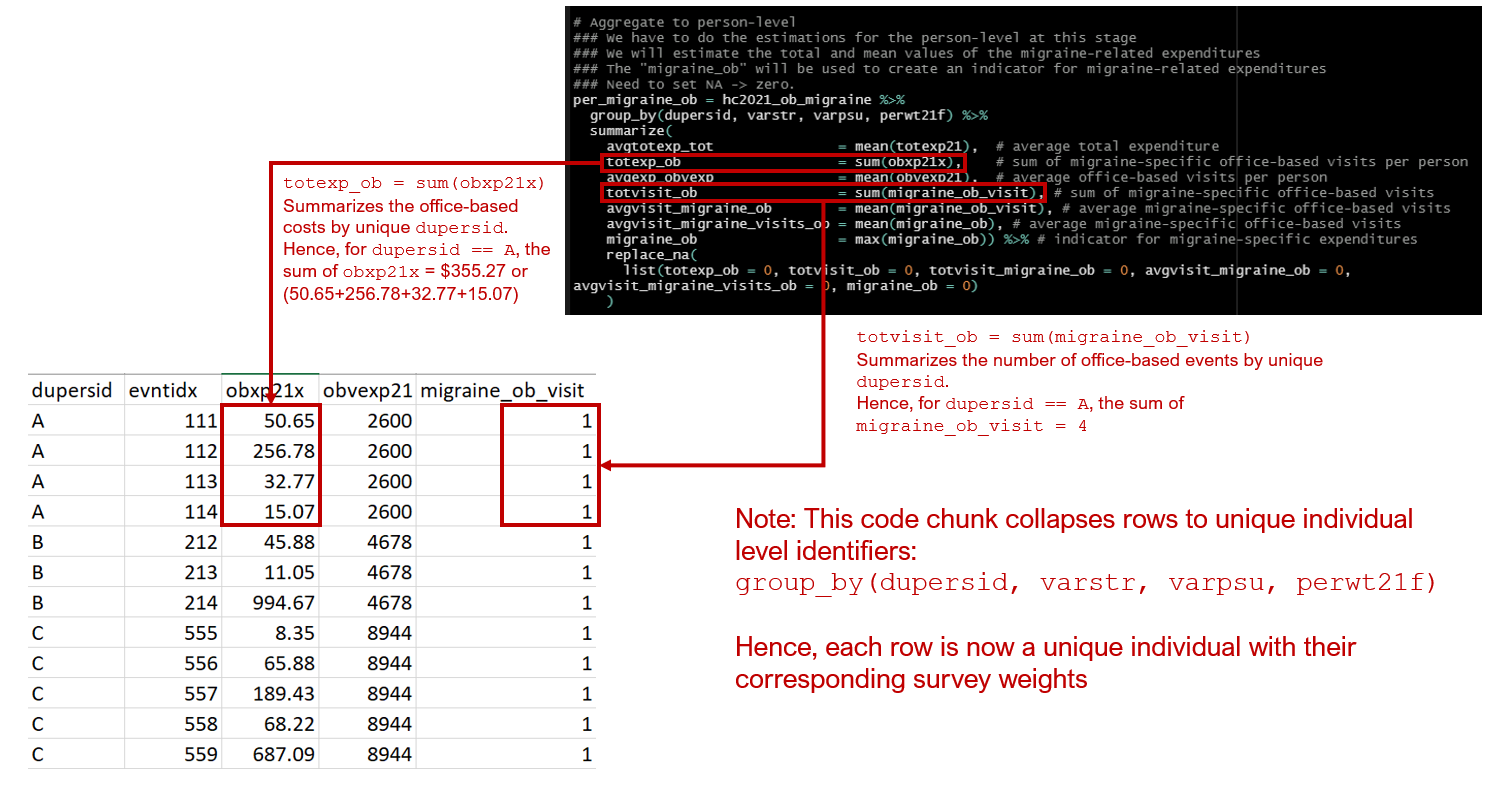
\includegraphics[width=1\linewidth]{Figure 4_3} \caption{Visual explanation of the code chunk}\label{fig:unnamed-chunk-48}
\end{figure}

Once this step is completed, you can check to see that the number of rows from the new dataframe (\texttt{per\_migraine\_ob}) is equal to the number of rows from the Full-Year Consolidated file (\texttt{hc2021}). They should be equal.

\begin{Shaded}
\begin{Highlighting}[]
\DocumentationTok{\#\#\# QC: Should have the same number as the full{-}year consolidated file}
\FunctionTok{nrow}\NormalTok{(per\_migraine\_ob) }\SpecialCharTok{==} \FunctionTok{nrow}\NormalTok{(hc2021)}
\end{Highlighting}
\end{Shaded}

\begin{verbatim}
## [1] TRUE
\end{verbatim}

Now that you've merged the migraine-specific office-based expenditures with the Full-Year Consolidated file, we can start on repeating this process for the migraine-specific inpatient expenditures.

\hypertarget{part-3---migraine-specific-inpatient-expenditures}{%
\subsection{Part 3 - Migraine-specific inpatient expenditures}\label{part-3---migraine-specific-inpatient-expenditures}}

The code for the migraine-specific inpatient expenditures is similar to the migraine-specific office-based expenditures so I won't go through them step-by-step. However, there are several important differences.

First, the inpatient event type is \texttt{eventype\ ==\ 4}, which needs to be included when you isolate the event types from the \texttt{clnk2021} file.

\begin{Shaded}
\begin{Highlighting}[]
\DocumentationTok{\#\#\#\#\#\#\#\#\#\#\#\#\#\#\#\#\#\#\#\#\#\#\#\#\#\#\#\#\#\#\#\#\#\#\#\#\#\#\#\#\#\#\#\#}
\DocumentationTok{\#\# INPATIENT STAYS}
\DocumentationTok{\#\#\#\#\#\#\#\#\#\#\#\#\#\#\#\#\#\#\#\#\#\#\#\#\#\#\#\#\#\#\#\#\#\#\#\#\#\#\#\#\#\#\#\#}
\CommentTok{\# Inpatient stays events}
\NormalTok{inpat\_events }\OtherTok{=}\NormalTok{ clnk2021 }\SpecialCharTok{\%\textgreater{}\%}
  \FunctionTok{filter}\NormalTok{(eventype }\SpecialCharTok{==} \DecValTok{4}\NormalTok{)}

\CommentTok{\# QC: Should only have EVENTYPE == 4}
\NormalTok{inpat\_events }\SpecialCharTok{\%\textgreater{}\%}
  \FunctionTok{count}\NormalTok{(eventype)}
\end{Highlighting}
\end{Shaded}

\begin{verbatim}
## # A tibble: 1 x 2
##   eventype                          n
##   <dbl+lbl>                     <int>
## 1 4 [4 INPATIENT HOSPITAL STAY]  3167
\end{verbatim}

\begin{Shaded}
\begin{Highlighting}[]
\CommentTok{\# Merge migraine diagnosis file with inpatient stays file}
\NormalTok{migraine\_lnk\_inpat }\OtherTok{=} \FunctionTok{inner\_join}\NormalTok{(}
\NormalTok{  migraine, inpat\_events,}
  \AttributeTok{by =} \FunctionTok{c}\NormalTok{(}\StringTok{"dupersid"}\NormalTok{, }\StringTok{"condidx"}\NormalTok{)}
\NormalTok{)}

\CommentTok{\# Select only DISTINCT events ("De{-}duplicate")}
\NormalTok{migraine\_inpat\_distinct }\OtherTok{=}\NormalTok{ migraine\_lnk\_inpat }\SpecialCharTok{\%\textgreater{}\%}
  \FunctionTok{distinct}\NormalTok{(dupersid, evntidx, eventype)}


\CommentTok{\# Merge inpatient stays file with distinct migraine{-}specific inpatient stays file}
\DocumentationTok{\#\#\# Use the inner\_join() to merge ob2021x and migraine\_inpat\_distinct dataframes}
\DocumentationTok{\#\#\# Then create a new indicator variable called "migraine\_inpat\_stays = 1."}
\NormalTok{inpat\_migraine }\OtherTok{=} \FunctionTok{inner\_join}\NormalTok{(}
\NormalTok{  inpat2021x, migraine\_inpat\_distinct) }\SpecialCharTok{\%\textgreater{}\%}
  \FunctionTok{mutate}\NormalTok{(}\AttributeTok{migraine\_inpat\_stays =} \DecValTok{1}\NormalTok{)}


\CommentTok{\# Merge with full{-}year consolidated file}
\DocumentationTok{\#\#\# Use the full\_join() to keep all the rows from both dataframes.}
\DocumentationTok{\#\#\# Then create a new object called hc2021\_inpat\_migraine}
\DocumentationTok{\#\#\# \& a new indicator variable called "migraine\_inpat = 1"}
\DocumentationTok{\#\#\# \& another new indicator variable called "fyc = 1."}
\DocumentationTok{\#\#\# Note: These are not unique rows (repeated dupersid)}
\NormalTok{hc2021\_inpat\_migraine }\OtherTok{=} \FunctionTok{full\_join}\NormalTok{(}
\NormalTok{  inpat\_migraine }\SpecialCharTok{\%\textgreater{}\%} \FunctionTok{mutate}\NormalTok{(}\AttributeTok{migraine\_inpat =} \DecValTok{1}\NormalTok{),}
\NormalTok{  hc2021x }\SpecialCharTok{\%\textgreater{}\%} \FunctionTok{mutate}\NormalTok{(}\AttributeTok{fyc =} \DecValTok{1}\NormalTok{)}
\NormalTok{)}


\CommentTok{\# Aggregate to person{-}level}
\DocumentationTok{\#\#\# We have to do the estimations for the person{-}level at this stage}
\DocumentationTok{\#\#\# We will estimate the total and mean values of the migraine{-}related expenditures}
\DocumentationTok{\#\#\# The "migraine\_inpat" will be used to create an indicator for migraine{-}related expenditures}
\DocumentationTok{\#\#\# Need to set NA {-}\textgreater{} zero.}
\NormalTok{per\_migraine\_inpat }\OtherTok{=}\NormalTok{ hc2021\_inpat\_migraine }\SpecialCharTok{\%\textgreater{}\%}
  \FunctionTok{group\_by}\NormalTok{(dupersid, varstr, varpsu, perwt21f) }\SpecialCharTok{\%\textgreater{}\%}
  \FunctionTok{summarize}\NormalTok{(}
    \AttributeTok{totnights\_inpat                =} \FunctionTok{sum}\NormalTok{(numnighx),}
    \AttributeTok{totexp\_inpat                   =} \FunctionTok{sum}\NormalTok{(ipxp21x),}
    \AttributeTok{avgexp\_iptexp                  =} \FunctionTok{mean}\NormalTok{(iptexp21),}
    \AttributeTok{totvisit\_inpat                 =} \FunctionTok{sum}\NormalTok{(migraine\_inpat\_stays),}
    \AttributeTok{avgvisit\_inpat                 =} \FunctionTok{mean}\NormalTok{(migraine\_inpat\_stays),}
    \AttributeTok{avgvisit\_migraine\_visits\_inpat =} \FunctionTok{mean}\NormalTok{(migraine\_inpat),}
    \AttributeTok{migraine\_inpat                 =} \FunctionTok{max}\NormalTok{(migraine\_inpat)) }\SpecialCharTok{\%\textgreater{}\%}
  \FunctionTok{replace\_na}\NormalTok{(}
    \FunctionTok{list}\NormalTok{(}\AttributeTok{totnights\_inpat =} \DecValTok{0}\NormalTok{, }\AttributeTok{totexp\_inpat =} \DecValTok{0}\NormalTok{, }\AttributeTok{totvisit\_inpat =} \DecValTok{0}\NormalTok{, }\AttributeTok{avgvisit\_inpat =} \DecValTok{0}\NormalTok{, }\AttributeTok{avgvisit\_migraine\_visits\_inpat =} \DecValTok{0}\NormalTok{, }\AttributeTok{migraine\_inpat =} \DecValTok{0}\NormalTok{)}
\NormalTok{  )}

\DocumentationTok{\#\#\# QC: Should have the same number as the full{-}year consolidated file}
\FunctionTok{nrow}\NormalTok{(per\_migraine\_inpat) }\SpecialCharTok{==} \FunctionTok{nrow}\NormalTok{(hc2021)}
\end{Highlighting}
\end{Shaded}

\begin{verbatim}
## [1] TRUE
\end{verbatim}

\hypertarget{part-4---combine-office-based-and-inpatient-expenditure-files}{%
\subsection{Part 4 - Combine office-based and inpatient expenditure files}\label{part-4---combine-office-based-and-inpatient-expenditure-files}}

Once you have the migraine-specific inpatient expenditures dataframe completed, you can start the process to combine this with the migraine-specific office-based expenditures dataframe.

First, we want to merge using the \texttt{left\_join} function the migraine-specific office-based expenditure dataframe with the Full-Year Consolidated file \texttt{hc2021x}. We do this because there were a couple of variables in \texttt{hc2021x} that we would like to keep such as the sex (\texttt{sex}) and race (\texttt{racev1x}) variables. We will call this new dataframe \texttt{combined\_data\_ob\_part}.

\begin{Shaded}
\begin{Highlighting}[]
\CommentTok{\# COMBINE OBVISIT AND INPAT {-} SPECIFIC EXPENDITURE FILES}
\DocumentationTok{\#\#\# Part 1: Combine the office{-}based visit exp file with the hc2021x file}
\NormalTok{combined\_data\_ob\_part }\OtherTok{\textless{}{-}} \FunctionTok{left\_join}\NormalTok{(}
\NormalTok{  hc2021x, }
\NormalTok{  per\_migraine\_ob,}
  \AttributeTok{by =} \FunctionTok{c}\NormalTok{(}\StringTok{"dupersid"}\NormalTok{, }\StringTok{"varstr"}\NormalTok{, }\StringTok{"varpsu"}\NormalTok{, }\StringTok{"perwt21f"}\NormalTok{)}
\NormalTok{)}
\end{Highlighting}
\end{Shaded}

Then, we want to merge the migraine-specific inpatient expenditures \texttt{per\_migraine\_inpat} to the dataframe \texttt{combined\_data\_ob\_part} to create a new dataframe called \texttt{combined\_data\_ob\_inpat\_part}.

\begin{Shaded}
\begin{Highlighting}[]
\DocumentationTok{\#\#\# Part 2: Combine the inpatient stays file with the "combined\_data\_ob\_part" file}
\NormalTok{combined\_data\_ob\_inpat\_part }\OtherTok{\textless{}{-}} \FunctionTok{left\_join}\NormalTok{(}
\NormalTok{  combined\_data\_ob\_part, }
\NormalTok{  per\_migraine\_inpat,}
  \AttributeTok{by =} \FunctionTok{c}\NormalTok{(}\StringTok{"dupersid"}\NormalTok{, }\StringTok{"varstr"}\NormalTok{, }\StringTok{"varpsu"}\NormalTok{, }\StringTok{"perwt21f"}\NormalTok{)}
\NormalTok{)}
\end{Highlighting}
\end{Shaded}

Once that part is completed, we will have a dataframe that includes both the migraine-specific office-based visit and inpatient stay expenditures.

Next, we will take this opportunity to create an indicator variable for individuals with a migraine diagnosis or condition. So far, we have identified and isolated office-based and inpatient expenditures that were migraine-specific. This means that some individuals with a migraine diagnosis may not have accrued any migraine-specific office-based or inpatient expenditures. It's possible that they have other expenditures, but those may not be migraine-specific. Hence, it is important that we create an indicator variable for those individuals with migraine in the comprehensive dataframe.

\begin{Shaded}
\begin{Highlighting}[]
\DocumentationTok{\#\#\# Part 3: Merge an indicator variable for migraine diagnosis. }
\DocumentationTok{\#\#\# Not all patients with migraine has an expenditure.}

\DocumentationTok{\#\#\# a) Create a dataframe with the dupersid and migraine indicator.}
\NormalTok{migraine\_distinct\_qc }\OtherTok{=}\NormalTok{ migraine }\SpecialCharTok{\%\textgreater{}\%} 
  \FunctionTok{distinct}\NormalTok{(dupersid) }\SpecialCharTok{\%\textgreater{}\%}
  \FunctionTok{mutate}\NormalTok{(}\AttributeTok{migraine\_indicator =} \DecValTok{1}\NormalTok{)}

\DocumentationTok{\#\#\# b) Merge "migraine\_distinct\_qc" to the larger table.}
\DocumentationTok{\#\#\# This will be a 1 to 1 join.}
\NormalTok{combined\_data\_migraine }\OtherTok{\textless{}{-}} \FunctionTok{left\_join}\NormalTok{(}
\NormalTok{  combined\_data\_ob\_inpat\_part,}
\NormalTok{  migraine\_distinct\_qc,}
  \AttributeTok{by =} \FunctionTok{c}\NormalTok{(}\StringTok{"dupersid"}\NormalTok{))}

\DocumentationTok{\#\#\# c) We also need to convert NA to 0 for the "migraine\_indicator" variable.}
\NormalTok{combined\_data\_migraine }\OtherTok{=}\NormalTok{ combined\_data\_migraine }\SpecialCharTok{\%\textgreater{}\%}
  \FunctionTok{replace\_na}\NormalTok{(}\FunctionTok{list}\NormalTok{(}\AttributeTok{migraine\_indicator =} \DecValTok{0}\NormalTok{))}
\end{Highlighting}
\end{Shaded}

\hypertarget{part-5---descriptive-analysis-using-survey-weights}{%
\subsection{Part 5 - Descriptive analysis using survey weights}\label{part-5---descriptive-analysis-using-survey-weights}}

There are many ways to describe the expenditures in the migraine population.

First, we need to invoke the survey design for our data using the \texttt{svydesign} function. We will call this the \texttt{survey\_cohort} design.

\begin{Shaded}
\begin{Highlighting}[]
\CommentTok{\# Define person{-}level survey design}
\NormalTok{survey\_cohort }\OtherTok{=} \FunctionTok{svydesign}\NormalTok{(}
  \AttributeTok{id =} \SpecialCharTok{\textasciitilde{}}\NormalTok{varpsu, }
  \AttributeTok{strata =} \SpecialCharTok{\textasciitilde{}}\NormalTok{varstr,}
  \AttributeTok{weights =} \SpecialCharTok{\textasciitilde{}}\NormalTok{perwt21f,}
  \AttributeTok{data =}\NormalTok{ combined\_data\_migraine,}
  \AttributeTok{nest =} \ConstantTok{TRUE}\NormalTok{)}
\end{Highlighting}
\end{Shaded}

Next, we can provide the average costs and amounts of office-based visit and inpatient stay expenditures for the whole cohort, both individuals with and without a migraine condition. We will use the \texttt{svyby} function to group the findings into those with migraine \texttt{migraine\_indicator\ ==\ 1} and those without migraine \texttt{migraine\_indicator\ ==\ 0}.

Note: We expect to see zero costs and amount for the non-migraine individuals.

\begin{Shaded}
\begin{Highlighting}[]
\DocumentationTok{\#\#\# Average migraine{-}specific office{-}based visit costs and amount}
\FunctionTok{svyby}\NormalTok{(}\SpecialCharTok{\textasciitilde{}}\NormalTok{totexp\_ob, }\SpecialCharTok{\textasciitilde{}}\NormalTok{migraine\_indicator, survey\_cohort, svymean)}
\end{Highlighting}
\end{Shaded}

\begin{verbatim}
##   migraine_indicator   totexp_ob          se
## 0                  0   0.0000000  0.00000000
## 1                  1 473.7215498 63.42344309
\end{verbatim}

\begin{Shaded}
\begin{Highlighting}[]
\FunctionTok{svyby}\NormalTok{(}\SpecialCharTok{\textasciitilde{}}\NormalTok{totvisit\_ob, }\SpecialCharTok{\textasciitilde{}}\NormalTok{migraine\_indicator, survey\_cohort, svymean)}
\end{Highlighting}
\end{Shaded}

\begin{verbatim}
##   migraine_indicator totvisit_ob           se
## 0                  0 0.000000000 0.0000000000
## 1                  1 1.874864152 0.2637829887
\end{verbatim}

\begin{Shaded}
\begin{Highlighting}[]
\DocumentationTok{\#\#\# Average migraine{-}specific inpatient costs and nights stayed}
\FunctionTok{svyby}\NormalTok{(}\SpecialCharTok{\textasciitilde{}}\NormalTok{totexp\_inpat, }\SpecialCharTok{\textasciitilde{}}\NormalTok{migraine\_indicator, survey\_cohort, svymean)}
\end{Highlighting}
\end{Shaded}

\begin{verbatim}
##   migraine_indicator totexp_inpat         se
## 0                  0   0.00000000  0.0000000
## 1                  1  69.78947691 37.9709726
\end{verbatim}

\begin{Shaded}
\begin{Highlighting}[]
\FunctionTok{svyby}\NormalTok{(}\SpecialCharTok{\textasciitilde{}}\NormalTok{totnights\_inpat, }\SpecialCharTok{\textasciitilde{}}\NormalTok{migraine\_indicator, survey\_cohort, svymean)}
\end{Highlighting}
\end{Shaded}

\begin{verbatim}
##   migraine_indicator totnights_inpat           se
## 0                  0   0.00000000000 0.0000000000
## 1                  1   0.02538119475 0.0133157815
\end{verbatim}

Based on these findings, the average cost for migraine-specific office-based visits was \$474 for individuals with a migraine condition. The average number of office-based events was 1.9 events per individual with a migraine condition.

The average migraine-specific inpatient stay expenditure was \$70 per individual with a migraine condition. The average migraine-specific inpatient nights was 0.025 nights per individual with a migraine condition.

Among individual without a migraine condition, the averages would have been zero.

Alternatively, we could have done this using a subset of the migraine cohort, but this will require us to create a subset of individuals with a migraine condition, which we will call \texttt{migraine\_cohort}.

\begin{Shaded}
\begin{Highlighting}[]
\CommentTok{\# Subgroup of individuals with inpatient stays for migraines}
\NormalTok{migraine\_cohort }\OtherTok{=} \FunctionTok{subset}\NormalTok{(survey\_cohort, migraine\_indicator }\SpecialCharTok{==} \DecValTok{1}\NormalTok{)}
\end{Highlighting}
\end{Shaded}

Once we have the subset, we can provide the mean migraine-specific office-based and inpatient expenditures. Comparing the results from the subset to the whole cohort, we find that for individuals with the migraine indicator \texttt{migraine\_indiciator\ ==\ 1}, the average costs and amount of office-based and inpatient expenditures are the same.

\begin{Shaded}
\begin{Highlighting}[]
\DocumentationTok{\#\#\# Average migraine{-}specific office{-}based visit costs and amount}
\FunctionTok{svyby}\NormalTok{(}\SpecialCharTok{\textasciitilde{}}\NormalTok{totexp\_ob, }\SpecialCharTok{\textasciitilde{}}\NormalTok{migraine\_indicator, migraine\_cohort, svymean)}
\end{Highlighting}
\end{Shaded}

\begin{verbatim}
##   migraine_indicator   totexp_ob          se
## 1                  1 473.7215498 63.42344309
\end{verbatim}

\begin{Shaded}
\begin{Highlighting}[]
\FunctionTok{svyby}\NormalTok{(}\SpecialCharTok{\textasciitilde{}}\NormalTok{totvisit\_ob, }\SpecialCharTok{\textasciitilde{}}\NormalTok{migraine\_indicator, migraine\_cohort, svymean)}
\end{Highlighting}
\end{Shaded}

\begin{verbatim}
##   migraine_indicator totvisit_ob           se
## 1                  1 1.874864152 0.2637829887
\end{verbatim}

\begin{Shaded}
\begin{Highlighting}[]
\DocumentationTok{\#\#\# Average migraine{-}specific inpatient costs and nights stayed}
\FunctionTok{svyby}\NormalTok{(}\SpecialCharTok{\textasciitilde{}}\NormalTok{totexp\_inpat, }\SpecialCharTok{\textasciitilde{}}\NormalTok{migraine\_indicator, migraine\_cohort, svymean)}
\end{Highlighting}
\end{Shaded}

\begin{verbatim}
##   migraine_indicator totexp_inpat         se
## 1                  1  69.78947691 37.9709726
\end{verbatim}

\begin{Shaded}
\begin{Highlighting}[]
\FunctionTok{svyby}\NormalTok{(}\SpecialCharTok{\textasciitilde{}}\NormalTok{totnights\_inpat, }\SpecialCharTok{\textasciitilde{}}\NormalTok{migraine\_indicator, migraine\_cohort, svymean)}
\end{Highlighting}
\end{Shaded}

\begin{verbatim}
##   migraine_indicator totnights_inpat           se
## 1                  1   0.02538119475 0.0133157815
\end{verbatim}

The average values for individuals with a migraine condition should be exactly the same in the subset and the whole cohort.

But what if we are interested in migraine-specific expenditures for only those individuals with a migraine AND non-zero expenditures? This would mean that we will have EXCLUDE individual with a migraine condition and ZERO expenditures.

We can do this with another subset.

The first subset we will do is the migraine-specific office-based visit. We will subset our migraine group from the \texttt{per\_migraine\_ob} dataframe and call it \texttt{migraine\_ob\_nonzero} to reflect the non-zero expenditures of the migraine only cohort. We'll all this subset \texttt{migraineOB}.

\begin{Shaded}
\begin{Highlighting}[]
\CommentTok{\# Define person{-}level survey design}
\NormalTok{migraine\_ob\_nonzero }\OtherTok{=} \FunctionTok{svydesign}\NormalTok{(}
  \AttributeTok{id =} \SpecialCharTok{\textasciitilde{}}\NormalTok{varpsu, }
  \AttributeTok{strata =} \SpecialCharTok{\textasciitilde{}}\NormalTok{varstr,}
  \AttributeTok{weights =} \SpecialCharTok{\textasciitilde{}}\NormalTok{perwt21f,}
  \AttributeTok{data =}\NormalTok{ per\_migraine\_ob,}
  \AttributeTok{nest =} \ConstantTok{TRUE}\NormalTok{)}

\CommentTok{\# Subgroup of individuals with office{-}based for migraines}
\NormalTok{migraineOB }\OtherTok{=} \FunctionTok{subset}\NormalTok{(migraine\_ob\_nonzero, migraine\_ob }\SpecialCharTok{==} \DecValTok{1}\NormalTok{)}
\end{Highlighting}
\end{Shaded}

Once we have the new subset, we can estimate the average expenditures for migraine-specific office-based visits.

\begin{Shaded}
\begin{Highlighting}[]
\FunctionTok{svymean}\NormalTok{(}\SpecialCharTok{\textasciitilde{}}\NormalTok{totexp\_ob, }\AttributeTok{design =}\NormalTok{ migraineOB) }\CommentTok{\# Mean office{-}based expenditures}
\end{Highlighting}
\end{Shaded}

\begin{verbatim}
##                mean        SE
## totexp_ob 988.27575 126.33587
\end{verbatim}

\begin{Shaded}
\begin{Highlighting}[]
\FunctionTok{svymean}\NormalTok{(}\SpecialCharTok{\textasciitilde{}}\NormalTok{totvisit\_ob, }\AttributeTok{design =}\NormalTok{ migraineOB) }\CommentTok{\# Mean migraine office{-}based visits}
\end{Highlighting}
\end{Shaded}

\begin{verbatim}
##                  mean     SE
## totvisit_ob 3.9113331 0.5329
\end{verbatim}

Based on these findings, among individuals with a migraine condition and non-zero migraine-specific expenditures, the average migraine-specific office-based costs was \$988 and the average number of migraine-specific office-based events was 3.9 events. This is very different from the \$474 and 1.9 office-based events previously reported for the migraine population.

We can also do this for the inpatient expenditures subset, which we will call \texttt{migraineINPAT}.

\begin{Shaded}
\begin{Highlighting}[]
\CommentTok{\# Define person{-}level survey design}
\NormalTok{migraine\_inpat\_nonzero }\OtherTok{=} \FunctionTok{svydesign}\NormalTok{(}
  \AttributeTok{id =} \SpecialCharTok{\textasciitilde{}}\NormalTok{varpsu, }
  \AttributeTok{strata =} \SpecialCharTok{\textasciitilde{}}\NormalTok{varstr,}
  \AttributeTok{weights =} \SpecialCharTok{\textasciitilde{}}\NormalTok{perwt21f,}
  \AttributeTok{data =}\NormalTok{ per\_migraine\_inpat,}
  \AttributeTok{nest =} \ConstantTok{TRUE}\NormalTok{)}
  
\CommentTok{\# Subgroup of individuals with office{-}based for migraines}
\NormalTok{migraineINPAT }\OtherTok{=} \FunctionTok{subset}\NormalTok{(migraine\_inpat\_nonzero, migraine\_inpat }\SpecialCharTok{==} \DecValTok{1}\NormalTok{)}

\FunctionTok{svymean}\NormalTok{(}\SpecialCharTok{\textasciitilde{}}\NormalTok{totexp\_inpat, }\AttributeTok{design =}\NormalTok{ migraineINPAT) }\CommentTok{\# Mean inpatient stays expenditures}
\end{Highlighting}
\end{Shaded}

\begin{verbatim}
##                   mean        SE
## totexp_inpat 7364.0586 1138.0975
\end{verbatim}

\begin{Shaded}
\begin{Highlighting}[]
\FunctionTok{svymean}\NormalTok{(}\SpecialCharTok{\textasciitilde{}}\NormalTok{totnights\_inpat, }\AttributeTok{design =}\NormalTok{ migraineINPAT) }\CommentTok{\# Mean inpatient stays nights }
\end{Highlighting}
\end{Shaded}

\begin{verbatim}
##                      mean      SE
## totnights_inpat 2.6781775 0.65583
\end{verbatim}

Based on these findings, among individuals with a migraine condition and non-zero migraine-specific expenditures, the average migraine-specific inpatient stay costs was \$7364 and the average number of nights stayed was 2.7 nights. This is very different from the \$70 and 0.025 nights previously reported for the migraine population.

Depending on how you define your cohort, these averages will be different.

There are 756 individuals with a migraine condition, but only 353 of those with a migraine-specific office-based visit expenditure and 7 of those with a migraine-specific inpatient stay expenditure.

A summary of the findings is provided below:

\begin{figure}
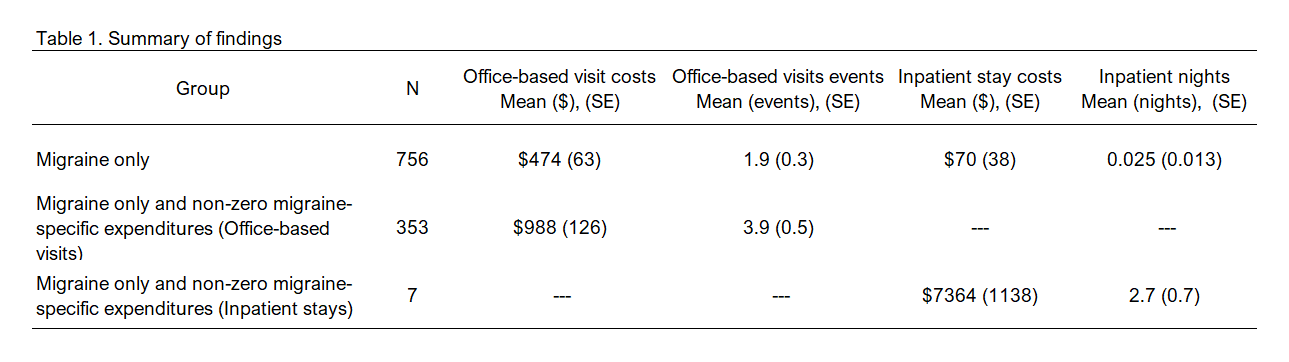
\includegraphics[width=1\linewidth]{Figure 4_4} \caption{Summary of findings.}\label{fig:unnamed-chunk-61}
\end{figure}

\hypertarget{conclusions-3}{%
\section{Conclusions}\label{conclusions-3}}

We can link events with specific conditions to get a more precise estimate of the expenditures. In this motivating example, we linked the migraine condition to its events and estimated the average office-based visit and inpatient stay expenditures. But we also explored the differences in these average when the denominator is restricted further to those with non-zero condition-specific expenditures. This process can be generalized to other conditions and other types of events.

\hypertarget{acknowledgements-3}{%
\section{Acknowledgements}\label{acknowledgements-3}}

This tutorial would not be possible with the resources provided by \href{https://github.com/HHS-AHRQ/MEPS}{AHRQ MEPS GitHub site}. The resources are amazing, and the codes are available for Stata, R, and SAS. Each exercise provide a new perspective on how to leverage the MEPS dataset for anyone's research or investigations. I highly encourage people to visit their site.

\hypertarget{work-in-progress}{%
\section{Work in progress}\label{work-in-progress}}

This is a work in progress so expect some updates in the future.

\hypertarget{disclaimers}{%
\section{Disclaimers}\label{disclaimers}}

Any errors or mistakes are those of the author.

This is only for educational purposes.

This was built under R version 4.2.2 ``Innocent and Trusting''

\hypertarget{trends}{%
\chapter{Simple trend analysis with linear models}\label{trends}}

\hypertarget{introduction-4}{%
\section{Introduction}\label{introduction-4}}

Analyzing trends can be a tricky matter. You have to consider many things such as the autoregressive correlation between values across the time interval or the seasonal effects that occur and are unrelated to the risk factor. All these issues contribute to the difficulty and challenge of trend analysis. However, there are simple ways to perform rudimentary trend analysis with linear models that might be useful for most stakeholders.

Linear models are useful because they are easy to interpret. There is no re-transformation needed, and the outputs are interpreted in terms of real units. Non-linear models may require re-transformation or some kind of adjustment to get the \(\beta\) coefficients to be interpretable in real units.

Although there are a lot of different models that take into consideration the strength of the correlation between values across time (e.g., generalized estimating equation models) or the random slope and intercepts of subjects and groups, we will use the linear effects model to interpret the trends of healthcare expenditure of a representative sample of the US non-institutionalized patients.

\hypertarget{motivating-example}{%
\section{Motivating example}\label{motivating-example}}

We will use data from the \href{https://meps.ahrq.gov/mepsweb/}{Agency for Healthcare Research and Quality (AHRQ) Medical Expenditure Panel Survey (MEPS)} data from 2016 to 2021. We will use R to perform the simple trend analysis.

\hypertarget{loading-the-libraries}{%
\subsection{Loading the libraries}\label{loading-the-libraries}}

There are several libraries that we'll need to install and then load.

\begin{Shaded}
\begin{Highlighting}[]
\DocumentationTok{\#\#\# step 1a: Load the MEPS package}
\FunctionTok{library}\NormalTok{(}\StringTok{"MEPS"}\NormalTok{) }\DocumentationTok{\#\# You need to load the library every time you restart R}

\DocumentationTok{\#\#\# Step 1b: Load the other libraries}
\FunctionTok{library}\NormalTok{(}\StringTok{"survey"}\NormalTok{)}
\FunctionTok{library}\NormalTok{(}\StringTok{"foreign"}\NormalTok{)}
\FunctionTok{library}\NormalTok{(}\StringTok{"dplyr"}\NormalTok{)}
\FunctionTok{library}\NormalTok{(}\StringTok{"ggplot2"}\NormalTok{)}
\FunctionTok{library}\NormalTok{(}\StringTok{"questionr"}\NormalTok{) }\CommentTok{\# remotes::install\_github("juba/questionr")}
\FunctionTok{library}\NormalTok{(}\StringTok{"lspline"}\NormalTok{)  }\CommentTok{\# devtools::install\_github("mbojan/lspline", build\_vignettes=TRUE)}
\FunctionTok{library}\NormalTok{(}\StringTok{"ggeffects"}\NormalTok{) }\CommentTok{\# remotes::install\_github("strengejacke/ggeffects")}
\FunctionTok{library}\NormalTok{(}\StringTok{"margins"}\NormalTok{)}
\FunctionTok{library}\NormalTok{(}\StringTok{"gtsummary"}\NormalTok{) }\CommentTok{\# remotes::install\_github("ddsjoberg/gtsummary")}
\FunctionTok{library}\NormalTok{(}\StringTok{"sjPlot"}\NormalTok{) }\CommentTok{\# plot marginal effects ("plot\_model" function)}
\end{Highlighting}
\end{Shaded}

\hypertarget{loading-data-into-the-r-environment}{%
\subsection{Loading data into the R environment}\label{loading-data-into-the-r-environment}}

There are two ways to load the data onto the R environment from AHRQ MEPS.

\begin{Shaded}
\begin{Highlighting}[]
\CommentTok{\# There are two ways to load data from AHRQ MEPS website:}
\DocumentationTok{\#\#\#\# Method 1: Load data from AHRQ MEPS website}
\NormalTok{hc2021 }\OtherTok{=} \FunctionTok{read\_MEPS}\NormalTok{(}\AttributeTok{file =} \StringTok{"h233"}\NormalTok{)}
\NormalTok{hc2020 }\OtherTok{=} \FunctionTok{read\_MEPS}\NormalTok{(}\AttributeTok{file =} \StringTok{"h224"}\NormalTok{)}
\NormalTok{hc2019 }\OtherTok{=} \FunctionTok{read\_MEPS}\NormalTok{(}\AttributeTok{file =} \StringTok{"h216"}\NormalTok{)}
\NormalTok{hc2018 }\OtherTok{=} \FunctionTok{read\_MEPS}\NormalTok{(}\AttributeTok{file =} \StringTok{"h209"}\NormalTok{)}
\NormalTok{hc2017 }\OtherTok{=} \FunctionTok{read\_MEPS}\NormalTok{(}\AttributeTok{file =} \StringTok{"h201"}\NormalTok{)}
\NormalTok{hc2016 }\OtherTok{=} \FunctionTok{read\_MEPS}\NormalTok{(}\AttributeTok{file =} \StringTok{"h192"}\NormalTok{)}


\DocumentationTok{\#\#\#\# Method 2: Load data from AHRQ MEPS website}
\NormalTok{hc2021 }\OtherTok{=} \FunctionTok{read\_MEPS}\NormalTok{(}\AttributeTok{year =} \DecValTok{2021}\NormalTok{, }\AttributeTok{type =} \StringTok{"FYC"}\NormalTok{)}
\NormalTok{hc2020 }\OtherTok{=} \FunctionTok{read\_MEPS}\NormalTok{(}\AttributeTok{year =} \DecValTok{2020}\NormalTok{, }\AttributeTok{type =} \StringTok{"FYC"}\NormalTok{)}
\NormalTok{hc2019 }\OtherTok{=} \FunctionTok{read\_MEPS}\NormalTok{(}\AttributeTok{year =} \DecValTok{2019}\NormalTok{, }\AttributeTok{type =} \StringTok{"FYC"}\NormalTok{)}
\NormalTok{hc2018 }\OtherTok{=} \FunctionTok{read\_MEPS}\NormalTok{(}\AttributeTok{year =} \DecValTok{2018}\NormalTok{, }\AttributeTok{type =} \StringTok{"FYC"}\NormalTok{)}
\NormalTok{hc2017 }\OtherTok{=} \FunctionTok{read\_MEPS}\NormalTok{(}\AttributeTok{year =} \DecValTok{2017}\NormalTok{, }\AttributeTok{type =} \StringTok{"FYC"}\NormalTok{)}
\NormalTok{hc2016 }\OtherTok{=} \FunctionTok{read\_MEPS}\NormalTok{(}\AttributeTok{year =} \DecValTok{2016}\NormalTok{, }\AttributeTok{type =} \StringTok{"FYC"}\NormalTok{)}
\end{Highlighting}
\end{Shaded}

Once the data have been loaded onto R, we can made some edits. The first edit I make is ensure that all column or variable names are in lower case.

\begin{Shaded}
\begin{Highlighting}[]
\DocumentationTok{\#\# Change column names to lowercase}
\FunctionTok{names}\NormalTok{(hc2021) }\OtherTok{\textless{}{-}} \FunctionTok{tolower}\NormalTok{(}\FunctionTok{names}\NormalTok{(hc2021))}
\FunctionTok{names}\NormalTok{(hc2020) }\OtherTok{\textless{}{-}} \FunctionTok{tolower}\NormalTok{(}\FunctionTok{names}\NormalTok{(hc2020))}
\FunctionTok{names}\NormalTok{(hc2019) }\OtherTok{\textless{}{-}} \FunctionTok{tolower}\NormalTok{(}\FunctionTok{names}\NormalTok{(hc2019))}
\FunctionTok{names}\NormalTok{(hc2018) }\OtherTok{\textless{}{-}} \FunctionTok{tolower}\NormalTok{(}\FunctionTok{names}\NormalTok{(hc2018))}
\FunctionTok{names}\NormalTok{(hc2017) }\OtherTok{\textless{}{-}} \FunctionTok{tolower}\NormalTok{(}\FunctionTok{names}\NormalTok{(hc2017))}
\FunctionTok{names}\NormalTok{(hc2016) }\OtherTok{\textless{}{-}} \FunctionTok{tolower}\NormalTok{(}\FunctionTok{names}\NormalTok{(hc2016))}
\end{Highlighting}
\end{Shaded}

\hypertarget{download-the-linkage-file}{%
\subsection{Download the linkage file}\label{download-the-linkage-file}}

Next, we need to download the pooled linkage file. This has the updated primary sampling unit and strata for the individual respondents. This is an important file because when we pool MEPS data from different years, the primary sampling unit and strata will change. We will need to merge this with our pooled data eventually, which will be discussed later in the tutorial.

\begin{Shaded}
\begin{Highlighting}[]
\CommentTok{\# We need the linkage file with the appropriate stratum of the primary sampling strata (STRA9621) and primary sampling unit (PSU9621). (Note: Each year, the linkage file sampling unit name changes)}
\NormalTok{linkage }\OtherTok{=} \FunctionTok{read\_MEPS}\NormalTok{(}\AttributeTok{type =} \StringTok{"Pooled linkage"}\NormalTok{) }
\FunctionTok{names}\NormalTok{(linkage) }\OtherTok{\textless{}{-}} \FunctionTok{tolower}\NormalTok{(}\FunctionTok{names}\NormalTok{(linkage)) }\CommentTok{\# change variable name to lower case}
\end{Highlighting}
\end{Shaded}

\hypertarget{creating-the-pooled-data-file}{%
\subsection{Creating the pooled data file}\label{creating-the-pooled-data-file}}

Now that we have the Full-Year Consolidated files from 2016 to 2021 and the pooled linkage files loaded onto the R environment, we can being to clean the data and merge them together.

We'll start by keeping only those variables that will be needed for our analysis. These include the following variables:

\begin{itemize}
\item
  \texttt{dupersid}: The unique identifier of the individual respondent
\item
  \texttt{panel}: The panel when the individual entered the MEPS round
\item
  \texttt{varstr}: The individual sampling strata
\item
  \texttt{varpsu}: The individual primary sampling unit
\item
  \texttt{sex}: The sex variable (1 = MALE, 2 = FEMALE)
\item
  \texttt{totexp}: The total healthcare costs per individual per year (Note: This variable name was changed from the year-specific total expenditure (e.g., \texttt{totexp17f} to \texttt{totexp} because we are pooling from multiple years)
\item
  \texttt{perwt}: The person weight for the individual in the sample (Note: This variable name was changed from the year-specific person weight (e.g., \texttt{perwt7f}) to \texttt{perwt} because we are pooling from multiple years)
\end{itemize}

We also created an indicator variable \texttt{year} to reflect the year the Full-Year Consolidated file was captured.

When we merge all the data, we created a new variable \texttt{poolwt} where we divide the \texttt{perwt} by the number of years used in the pooled data (e.g., 6). This will generate a new individual person weight with the pooled data.

Note: For more instruction and information about pooling multiple years with MEPS data, please see the \href{https://meps.ahrq.gov/data_stats/download_data/pufs/h36/h36u15doc.shtml}{1996-2015 Pooled Linkage Variance Estimation File}. This document provides a good summary and documentation on creating a \texttt{poolwt} variable and using the pooled strata and primary sampling unit.

\begin{Shaded}
\begin{Highlighting}[]
\CommentTok{\# Select specific variables}

\DocumentationTok{\#\#\# 2021}
\NormalTok{hc2021p }\OtherTok{=}\NormalTok{ hc2021 }\SpecialCharTok{\%\textgreater{}\%}
  \FunctionTok{rename}\NormalTok{(}
    \AttributeTok{perwt =}\NormalTok{ perwt21f,}
    \AttributeTok{totexp =}\NormalTok{ totexp21) }\SpecialCharTok{\%\textgreater{}\%}
  \FunctionTok{select}\NormalTok{(}
\NormalTok{    dupersid, }
\NormalTok{    panel, }
\NormalTok{    varstr, }
\NormalTok{    varpsu,}
\NormalTok{    perwt,}
\NormalTok{    sex,}
\NormalTok{    totexp)}
\NormalTok{hc2021p}\SpecialCharTok{$}\NormalTok{year }\OtherTok{\textless{}{-}} \DecValTok{2021}

\DocumentationTok{\#\#\# 2020}
\NormalTok{hc2020p }\OtherTok{=}\NormalTok{ hc2020 }\SpecialCharTok{\%\textgreater{}\%}
  \FunctionTok{rename}\NormalTok{(}
    \AttributeTok{perwt =}\NormalTok{ perwt20f,}
    \AttributeTok{totexp =}\NormalTok{ totexp20) }\SpecialCharTok{\%\textgreater{}\%}
  \FunctionTok{select}\NormalTok{(}
\NormalTok{    dupersid, }
\NormalTok{    panel, }
\NormalTok{    varstr, }
\NormalTok{    varpsu,}
\NormalTok{    perwt,}
\NormalTok{    sex,}
\NormalTok{    totexp)}
\NormalTok{hc2020p}\SpecialCharTok{$}\NormalTok{year }\OtherTok{\textless{}{-}} \DecValTok{2020}


\DocumentationTok{\#\#\# 2019}
\NormalTok{hc2019p }\OtherTok{=}\NormalTok{ hc2019 }\SpecialCharTok{\%\textgreater{}\%}
  \FunctionTok{rename}\NormalTok{(}
    \AttributeTok{perwt =}\NormalTok{ perwt19f,}
    \AttributeTok{totexp =}\NormalTok{ totexp19) }\SpecialCharTok{\%\textgreater{}\%}
  \FunctionTok{select}\NormalTok{(}
\NormalTok{    dupersid, }
\NormalTok{    panel, }
\NormalTok{    varstr, }
\NormalTok{    varpsu,}
\NormalTok{    perwt,}
\NormalTok{    sex,}
\NormalTok{    totexp)}
\NormalTok{hc2019p}\SpecialCharTok{$}\NormalTok{year }\OtherTok{\textless{}{-}} \DecValTok{2019}

\DocumentationTok{\#\#\# 2018}
\NormalTok{hc2018p }\OtherTok{=}\NormalTok{ hc2018 }\SpecialCharTok{\%\textgreater{}\%}
  \FunctionTok{rename}\NormalTok{(}
    \AttributeTok{perwt =}\NormalTok{ perwt18f,}
    \AttributeTok{totexp =}\NormalTok{ totexp18) }\SpecialCharTok{\%\textgreater{}\%}
  \FunctionTok{select}\NormalTok{(}
\NormalTok{    dupersid, }
\NormalTok{    panel, }
\NormalTok{    varstr, }
\NormalTok{    varpsu,}
\NormalTok{    perwt,}
\NormalTok{    sex,}
\NormalTok{    totexp)}
\NormalTok{hc2018p}\SpecialCharTok{$}\NormalTok{year }\OtherTok{\textless{}{-}} \DecValTok{2018}

\DocumentationTok{\#\#\# 2017}
\NormalTok{hc2017p }\OtherTok{=}\NormalTok{ hc2017 }\SpecialCharTok{\%\textgreater{}\%}
  \FunctionTok{rename}\NormalTok{(}
    \AttributeTok{perwt =}\NormalTok{ perwt17f,}
    \AttributeTok{totexp =}\NormalTok{ totexp17) }\SpecialCharTok{\%\textgreater{}\%}
  \FunctionTok{select}\NormalTok{(}
\NormalTok{    dupersid, }
\NormalTok{    panel, }
\NormalTok{    varstr, }
\NormalTok{    varpsu,}
\NormalTok{    perwt,}
\NormalTok{    sex,}
\NormalTok{    totexp)}
\NormalTok{hc2017p}\SpecialCharTok{$}\NormalTok{year }\OtherTok{\textless{}{-}} \DecValTok{2017}

\DocumentationTok{\#\#\# 2016}
\NormalTok{hc2016p }\OtherTok{=}\NormalTok{ hc2016 }\SpecialCharTok{\%\textgreater{}\%}
  \FunctionTok{rename}\NormalTok{(}
    \AttributeTok{perwt =}\NormalTok{ perwt16f,}
    \AttributeTok{totexp =}\NormalTok{ totexp16) }\SpecialCharTok{\%\textgreater{}\%}
  \FunctionTok{select}\NormalTok{(}
\NormalTok{    dupersid, }
\NormalTok{    panel, }
\NormalTok{    varstr, }
\NormalTok{    varpsu,}
\NormalTok{    perwt,}
\NormalTok{    sex,}
\NormalTok{    totexp)}
\NormalTok{hc2016p}\SpecialCharTok{$}\NormalTok{year }\OtherTok{\textless{}{-}} \DecValTok{2016}


\CommentTok{\# Merge data and adjust the person weight by 6 years}
\NormalTok{pool\_data }\OtherTok{=} \FunctionTok{bind\_rows}\NormalTok{(hc2021p, }
\NormalTok{                      hc2020p,}
\NormalTok{                      hc2019p,}
\NormalTok{                      hc2018p,}
\NormalTok{                      hc2017p,}
\NormalTok{                      hc2016p) }\SpecialCharTok{\%\textgreater{}\%}
  \FunctionTok{mutate}\NormalTok{(}\AttributeTok{poolwt =}\NormalTok{ perwt }\SpecialCharTok{/} \DecValTok{6}\NormalTok{)}
\end{Highlighting}
\end{Shaded}

\hypertarget{merging-with-pooled-survey-primary-sampling-strata-and-unit}{%
\subsection{Merging with pooled survey primary sampling strata and unit}\label{merging-with-pooled-survey-primary-sampling-strata-and-unit}}

Next, we need to merge the pooled years file with the updated primary sampling strata and unit from the linkage file. The linkage file is updated every year. Since the latest Full-Year Consolidated Data file that we are using includes 2021, we are using the 2021 linkage file (\texttt{HC-229I}).

We first limit the linkage file to only include the following variables:

\begin{itemize}
\item
  \texttt{dupersid}: The unique identifier for the individual respondent (Note: We will need this to merge the files later)
\item
  \texttt{panel}: The panel when the individual entered the MEPS round (Note: We will need to use this to merge the files later)
\item
  \texttt{stra9621}: The pooled sampling strata
\item
  \texttt{psu9621}: The pooled primary sampling unit
\end{itemize}

\begin{Shaded}
\begin{Highlighting}[]
\CommentTok{\# Reduce the linkage file to only include dupersid, panel, stra9621, psu9621}
\NormalTok{linkage\_file }\OtherTok{=}\NormalTok{ linkage }\SpecialCharTok{\%\textgreater{}\%}
  \FunctionTok{select}\NormalTok{(dupersid, panel, stra9621, psu9621)}

\CommentTok{\# Merge link file with main data}
\NormalTok{pool\_data\_linked }\OtherTok{=} \FunctionTok{left\_join}\NormalTok{(pool\_data,}
\NormalTok{                             linkage\_file, }
                             \AttributeTok{by =} \FunctionTok{c}\NormalTok{(}\StringTok{"dupersid"}\NormalTok{, }\StringTok{"panel"}\NormalTok{))}
\end{Highlighting}
\end{Shaded}

\hypertarget{create-factor-variables}{%
\subsection{Create factor variables}\label{create-factor-variables}}

We need to create factor variables so that we can evaluate the marginal effects. Disclaimer: I'm not sure if this is always necessary. However, I run into issues with the \texttt{margins} package when I estimated the average marginal effects in R. I get errors about the size of the dimension or vector, which indicates that the dimensions of the dataframe is not correct. I'm not sure why this error occurs, but I seem to have avoided it when I convert my categorical variables into factors. I'm not sure if this is a bug in the \texttt{margins} package or something I did with the terms in the regression model, but I'll monitor and update this tutorial if there are any changes or discoveries. For now, we'll convert our categorical variables into factors. Here, I also convert the variable \texttt{year} into a factor.

\begin{Shaded}
\begin{Highlighting}[]
\CommentTok{\# Create factor variables:}
\DocumentationTok{\#\#\# MALE}
\NormalTok{pool\_data\_linked}\SpecialCharTok{$}\NormalTok{male[pool\_data\_linked}\SpecialCharTok{$}\NormalTok{sex }\SpecialCharTok{==} \DecValTok{1}\NormalTok{] }\OtherTok{=} \DecValTok{1}
\NormalTok{pool\_data\_linked}\SpecialCharTok{$}\NormalTok{male[pool\_data\_linked}\SpecialCharTok{$}\NormalTok{sex }\SpecialCharTok{==} \DecValTok{2}\NormalTok{] }\OtherTok{=} \DecValTok{0}
\FunctionTok{table}\NormalTok{(pool\_data\_linked}\SpecialCharTok{$}\NormalTok{male)}
\end{Highlighting}
\end{Shaded}

\begin{verbatim}
## 
##     0     1 
## 95023 86626
\end{verbatim}

\begin{Shaded}
\begin{Highlighting}[]
\NormalTok{pool\_data\_linked}\SpecialCharTok{$}\NormalTok{male }\OtherTok{\textless{}{-}} \FunctionTok{factor}\NormalTok{(pool\_data\_linked}\SpecialCharTok{$}\NormalTok{male, }\AttributeTok{levels =} \FunctionTok{c}\NormalTok{(}\DecValTok{0}\NormalTok{, }\DecValTok{1}\NormalTok{))}
\FunctionTok{class}\NormalTok{(pool\_data\_linked}\SpecialCharTok{$}\NormalTok{male)}
\end{Highlighting}
\end{Shaded}

\begin{verbatim}
## [1] "factor"
\end{verbatim}

\begin{Shaded}
\begin{Highlighting}[]
\FunctionTok{levels}\NormalTok{(pool\_data\_linked}\SpecialCharTok{$}\NormalTok{male)}
\end{Highlighting}
\end{Shaded}

\begin{verbatim}
## [1] "0" "1"
\end{verbatim}

\begin{Shaded}
\begin{Highlighting}[]
\DocumentationTok{\#\#\# YEAR}
\NormalTok{pool\_data\_linked}\SpecialCharTok{$}\NormalTok{year }\OtherTok{\textless{}{-}} \FunctionTok{factor}\NormalTok{(pool\_data\_linked}\SpecialCharTok{$}\NormalTok{year, }\AttributeTok{levels =} \FunctionTok{c}\NormalTok{(}\DecValTok{2016}\NormalTok{, }\DecValTok{2017}\NormalTok{, }\DecValTok{2018}\NormalTok{, }\DecValTok{2019}\NormalTok{, }\DecValTok{2020}\NormalTok{, }\DecValTok{2021}\NormalTok{))}
\FunctionTok{class}\NormalTok{(pool\_data\_linked}\SpecialCharTok{$}\NormalTok{year)}
\end{Highlighting}
\end{Shaded}

\begin{verbatim}
## [1] "factor"
\end{verbatim}

\begin{Shaded}
\begin{Highlighting}[]
\FunctionTok{levels}\NormalTok{(pool\_data\_linked}\SpecialCharTok{$}\NormalTok{year)}
\end{Highlighting}
\end{Shaded}

\begin{verbatim}
## [1] "2016" "2017" "2018" "2019" "2020" "2021"
\end{verbatim}

\hypertarget{set-the-survey-options}{%
\subsection{Set the survey options}\label{set-the-survey-options}}

Next, we set the survey options so that we can estimate the survey-weighted values for our population.

\begin{Shaded}
\begin{Highlighting}[]
\DocumentationTok{\#\#\#\#\#\#\#\#\#\#\#\#\#\#\#\#\#\#\#\#\#\#\#\#\#\#\#\#\#\#\#\#\# SURVEY \#\#\#\#\#\#\#\#\#\#\#\#\#\#\#\#\#\#\#\#\#\#\#\#\#\#\#\#\#\#\#\#\# }

\CommentTok{\# Set the survey options}
\FunctionTok{options}\NormalTok{(}\AttributeTok{survey.lonely.psu =} \StringTok{"adjust"}\NormalTok{)}
\FunctionTok{options}\NormalTok{(}\AttributeTok{survey.adjust.domain.lonely =} \ConstantTok{TRUE}\NormalTok{)}


\CommentTok{\# Define the survey design}
\NormalTok{survey\_design }\OtherTok{=} \FunctionTok{svydesign}\NormalTok{(}
  \AttributeTok{id =} \SpecialCharTok{\textasciitilde{}}\NormalTok{psu9621,}
  \AttributeTok{strata =} \SpecialCharTok{\textasciitilde{}}\NormalTok{stra9621,}
  \AttributeTok{weights =} \SpecialCharTok{\textasciitilde{}}\NormalTok{poolwt,}
  \AttributeTok{data =}\NormalTok{ pool\_data\_linked,}
  \AttributeTok{nest =} \ConstantTok{TRUE}\NormalTok{)}
\end{Highlighting}
\end{Shaded}

\hypertarget{trend-analysis---plot-the-total-healthcare-costs-by-sex-across-time}{%
\subsection{Trend analysis - Plot the total healthcare costs by sex across time}\label{trend-analysis---plot-the-total-healthcare-costs-by-sex-across-time}}

We can look at the total healthcare costs \texttt{totexp} by \texttt{sex} across time \texttt{year} with the \texttt{ggsurvey} function, which is part of the \texttt{questionr} package.

Visualizing the trends, females have a higher average total healthcare costs compared to males, and these are increasing across time. (Note: This trend was generated with the survey weights.)

\begin{Shaded}
\begin{Highlighting}[]
\DocumentationTok{\#\#\#\#\#\#\#\#\#\#\#\#\#\#\#\#\#\#\#\#\#\#\#\#\#\#\#\#\#\#\#\# TREND ANALYSIS \#\#\#\#\#\#\#\#\#\#\#\#\#\#\#\#\#\#\#\#\#\#\#\#\#\#\#\#\#\#\#\# }

\CommentTok{\# Plot total expenditures over time (Load the "questionr" package to use "ggsurvey")}
\FunctionTok{ggsurvey}\NormalTok{(survey\_design) }\SpecialCharTok{+}
  \FunctionTok{aes}\NormalTok{(}\AttributeTok{x =}\NormalTok{ year, }\AttributeTok{y =}\NormalTok{ totexp, }\AttributeTok{group =} \FunctionTok{factor}\NormalTok{(male), }\AttributeTok{color =} \FunctionTok{factor}\NormalTok{(male)) }\SpecialCharTok{+}
  \FunctionTok{stat\_summary}\NormalTok{(}\AttributeTok{fun =} \StringTok{"mean"}\NormalTok{, }\AttributeTok{geom =} \StringTok{"point"}\NormalTok{, }\AttributeTok{size =} \DecValTok{5}\NormalTok{) }\SpecialCharTok{+} 
  \FunctionTok{stat\_summary}\NormalTok{(}\AttributeTok{fun =} \StringTok{"mean"}\NormalTok{, }\AttributeTok{geom =} \StringTok{"line"}\NormalTok{, }\AttributeTok{size =} \DecValTok{1}\NormalTok{) }
\end{Highlighting}
\end{Shaded}

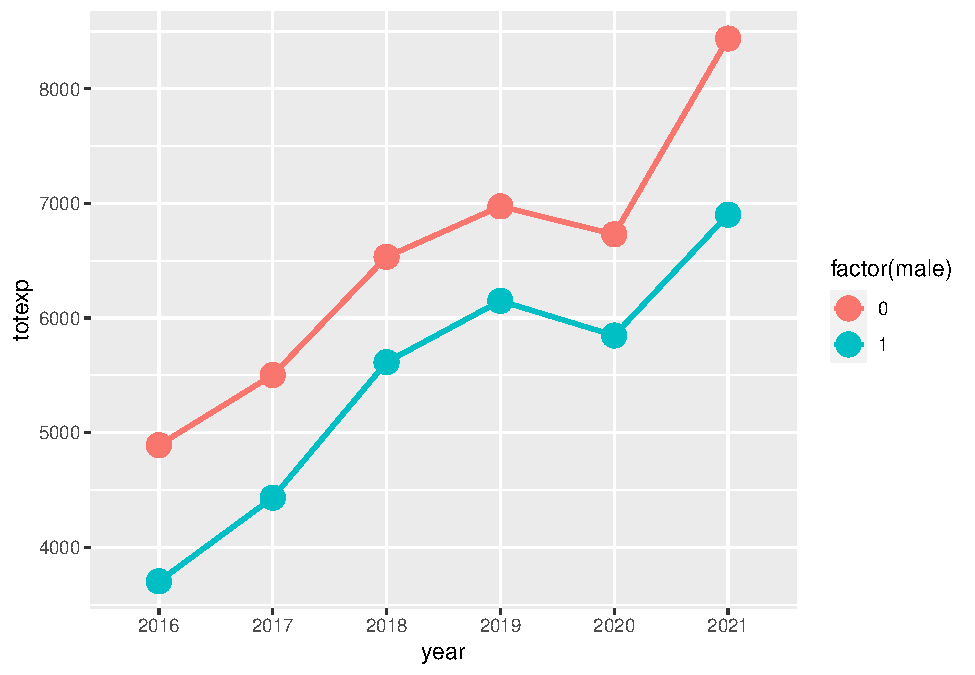
\includegraphics{_main_files/figure-latex/unnamed-chunk-70-1.pdf}

\hypertarget{regression-model}{%
\subsection{Regression model}\label{regression-model}}

We construct a linear regression model using the \texttt{svyglm} function in R. We included the terms \texttt{sex} and \texttt{year}, and we included an interaction term \texttt{sex:year}. This interaction term provides the estimates that describe the differences in the healthcare total costs between males and females when the years changes.

\begin{Shaded}
\begin{Highlighting}[]
\CommentTok{\# Survey{-}weight GLM model with interaction term}
\NormalTok{survey\_model }\OtherTok{\textless{}{-}} \FunctionTok{svyglm}\NormalTok{(totexp }\SpecialCharTok{\textasciitilde{}} \FunctionTok{factor}\NormalTok{(male) }\SpecialCharTok{+} \FunctionTok{factor}\NormalTok{(year) }\SpecialCharTok{+} \FunctionTok{factor}\NormalTok{(male)}\SpecialCharTok{:}\FunctionTok{factor}\NormalTok{(year), survey\_design)}
\end{Highlighting}
\end{Shaded}

We can view the estimates with their corresponding 95\% confidence intervals (CIs).

\begin{Shaded}
\begin{Highlighting}[]
\CommentTok{\# Summary table with 95\% CI}
\FunctionTok{round}\NormalTok{(}
  \FunctionTok{cbind}\NormalTok{(}
    \FunctionTok{summary}\NormalTok{(survey\_model, }\AttributeTok{df.resid =} \FunctionTok{degf}\NormalTok{(survey\_model}\SpecialCharTok{$}\NormalTok{survey.design))}\SpecialCharTok{$}\NormalTok{coef, }
    \FunctionTok{confint}\NormalTok{(survey\_model, }\AttributeTok{df       =} \FunctionTok{degf}\NormalTok{(survey\_model}\SpecialCharTok{$}\NormalTok{survey.design))}
\NormalTok{  ), }\DecValTok{4}\NormalTok{)}
\end{Highlighting}
\end{Shaded}

\begin{verbatim}
##                                  Estimate Std. Error t value Pr(>|t|)
## (Intercept)                     5632.6497   153.3156 36.7389   0.0000
## factor(male)1                  -1280.8517   183.1791 -6.9923   0.0000
## factor(year)2017                 164.5324   200.4297  0.8209   0.4121
## factor(year)2018                 981.6884   231.2365  4.2454   0.0000
## factor(year)2019                1103.9018   220.8327  4.9988   0.0000
## factor(year)2020                1022.3480   255.6661  3.9988   0.0001
## factor(year)2021                1964.5098   279.9440  7.0175   0.0000
## factor(male)1:factor(year)2017   276.5807   250.6373  1.1035   0.2704
## factor(male)1:factor(year)2018   154.8177   277.8425  0.5572   0.5776
## factor(male)1:factor(year)2019   291.3151   276.8655  1.0522   0.2932
## factor(male)1:factor(year)2020   487.1318   353.7995  1.3769   0.1692
## factor(male)1:factor(year)2021   -65.6524   403.7881 -0.1626   0.8709
##                                     2.5 %    97.5 %
## (Intercept)                     5331.3906 5933.9088
## factor(male)1                  -1640.7914 -920.9121
## factor(year)2017                -229.3041  558.3688
## factor(year)2018                 527.3179 1436.0589
## factor(year)2019                 669.9743 1537.8294
## factor(year)2020                 519.9744 1524.7217
## factor(year)2021                1414.4311 2514.5886
## factor(male)1:factor(year)2017  -215.9115  769.0730
## factor(male)1:factor(year)2018  -391.1317  700.7671
## factor(male)1:factor(year)2019  -252.7145  835.3448
## factor(male)1:factor(year)2020  -208.0701 1182.3338
## factor(male)1:factor(year)2021  -859.0800  727.7751
\end{verbatim}

A nicer way of presenting the regression model output is with the \texttt{tbl\_regression} function from the \texttt{gtsummary} package.

\begin{Shaded}
\begin{Highlighting}[]
\CommentTok{\# Use gtsummary to generate a clean summary table.}
\NormalTok{survey\_model }\SpecialCharTok{\%\textgreater{}\%}
  \FunctionTok{tbl\_regression}\NormalTok{(}\AttributeTok{intercept =} \ConstantTok{FALSE}\NormalTok{, }
                 \AttributeTok{estimate\_fun =} \ControlFlowTok{function}\NormalTok{(x) }\FunctionTok{style\_sigfig}\NormalTok{(x, }\AttributeTok{digits =} \DecValTok{3}\NormalTok{),}
                 \AttributeTok{pvalue\_fun =} \ControlFlowTok{function}\NormalTok{(x) }\FunctionTok{style\_sigfig}\NormalTok{(x, }\AttributeTok{digits =} \DecValTok{3}\NormalTok{)) }\SpecialCharTok{\%\textgreater{}\%}
  \FunctionTok{modify\_caption}\NormalTok{(}\StringTok{"Survey{-}weighted linear regression"}\NormalTok{)}
\end{Highlighting}
\end{Shaded}

\begin{table}

\caption{\label{tab:unnamed-chunk-73}Survey-weighted linear regression}
\centering
\begin{tabular}[t]{l|c|c|c}
\hline
**Characteristic** & **Beta** & **95\% CI** & **p-value**\\
\hline
factor(male) &  &  & \\
\hline
0 & — & — & \\
\hline
1 & -1,281 & -1,641, -921 & 0.000\\
\hline
factor(year) &  &  & \\
\hline
2016 & — & — & \\
\hline
2017 & 165 & -229, 558 & 0.412\\
\hline
2018 & 982 & 527, 1,436 & 0.000\\
\hline
2019 & 1,104 & 670, 1,538 & 0.000\\
\hline
2020 & 1,022 & 520, 1,525 & 0.000\\
\hline
2021 & 1,965 & 1,414, 2,515 & 0.000\\
\hline
factor(male) * factor(year) &  &  & \\
\hline
1 * 2017 & 277 & -216, 769 & 0.270\\
\hline
1 * 2018 & 155 & -391, 701 & 0.578\\
\hline
1 * 2019 & 291 & -253, 835 & 0.293\\
\hline
1 * 2020 & 487 & -208, 1,182 & 0.169\\
\hline
1 * 2021 & -65.7 & -859, 728 & 0.871\\
\hline
\end{tabular}
\end{table}

From these findings, we can make several interpretations.

The most important estimates are the interaction terms. These provide the estimation or the change in healthcare total costs between males and females due to an increase in the year. For instance, the interaction term \texttt{factor(male)1:factor(year)2017} is interpreted as the average difference in the change in total healthcare costs between males and females when the year increased from 2016 to 2017. This difference in the changes in total healthcare costs between males and females is \$276.58 (95\% CI: -\$215.91, \$769.07), which was not statistically significant.

\hypertarget{average-marginal-effects-between-males-and-females-at-each-year}{%
\subsection{Average marginal effects between males and females at each year}\label{average-marginal-effects-between-males-and-females-at-each-year}}

We can generate the average marginal effects or the differences in total healthcare costs between males and females at each year using the \texttt{margins} function.

For instance, the difference in total healthcare costs between males and females in 2019 was -\$990; 95\% CI: -\$1,396, -\$583, which was statistically significant. This means that males had lower average total healthcare costs compared to females in 2019.

\begin{Shaded}
\begin{Highlighting}[]
\CommentTok{\# Equivalent to Stata\textquotesingle{}s margin, dydx(year), at(male = 0:1)}
\NormalTok{margins1 }\OtherTok{\textless{}{-}} \FunctionTok{margins}\NormalTok{(survey\_model, }\AttributeTok{type =} \StringTok{"response"}\NormalTok{, }\AttributeTok{design =}\NormalTok{ survey\_design, }\AttributeTok{at =} \FunctionTok{list}\NormalTok{(}\AttributeTok{year =} \FunctionTok{c}\NormalTok{(}\DecValTok{2016}\NormalTok{, }\DecValTok{2017}\NormalTok{, }\DecValTok{2018}\NormalTok{, }\DecValTok{2019}\NormalTok{, }\DecValTok{2020}\NormalTok{, }\DecValTok{2021}\NormalTok{)), }\AttributeTok{variables =} \StringTok{"male"}\NormalTok{)}
\FunctionTok{summary}\NormalTok{(margins1)}
\end{Highlighting}
\end{Shaded}

\begin{verbatim}
##  factor      year        AME       SE       z      p      lower     upper
##   male1 2016.0000 -1280.8517 183.1789 -6.9924 0.0000 -1639.8757 -921.8278
##   male1 2017.0000 -1004.2710 188.0103 -5.3416 0.0000 -1372.7644 -635.7776
##   male1 2018.0000 -1126.0341 208.9060 -5.3901 0.0000 -1535.4823 -716.5859
##   male1 2019.0000  -989.5366 207.6048 -4.7664 0.0000 -1396.4346 -582.6386
##   male1 2020.0000  -793.7199 302.6867 -2.6222 0.0087 -1386.9749 -200.4649
##   male1 2021.0000 -1346.5042 359.8470 -3.7419 0.0002 -2051.7913 -641.2170
\end{verbatim}

\hypertarget{average-marginal-effects-between-years-for-males-and-females}{%
\subsection{Average marginal effects between years for males and females}\label{average-marginal-effects-between-years-for-males-and-females}}

Alternatively, we can estimate the average marginal effects or the changes in total healthcare costs between years for males and females.

For instance, in 2021, males had an average total healthcare cost of \$1965; 95\% CI: \$1,416, \$2,513, and females had an average total healthcare cost of \$1,899; 95\% CI: \$1277, \$2521.

\begin{Shaded}
\begin{Highlighting}[]
\CommentTok{\# Equivalent to Stata\textquotesingle{}s margin, dydx(year), at(male = 0:1)}
\NormalTok{margins2 }\OtherTok{\textless{}{-}} \FunctionTok{margins}\NormalTok{(survey\_model, }\AttributeTok{type =} \StringTok{"response"}\NormalTok{, }\AttributeTok{design =}\NormalTok{ survey\_design, }\AttributeTok{at =} \FunctionTok{list}\NormalTok{(}\AttributeTok{male =} \DecValTok{0}\SpecialCharTok{:}\DecValTok{1}\NormalTok{), }\AttributeTok{variables =} \StringTok{"year"}\NormalTok{)}
\FunctionTok{summary}\NormalTok{(margins2)}
\end{Highlighting}
\end{Shaded}

\begin{verbatim}
##    factor   male       AME       SE      z      p     lower     upper
##  year2017 0.0000  164.5324 200.4294 0.8209 0.4117 -228.3021  557.3669
##  year2017 1.0000  441.1131 190.2654 2.3184 0.0204   68.1998  814.0265
##  year2018 0.0000  981.6884 231.2367 4.2454 0.0000  528.4728 1434.9040
##  year2018 1.0000 1136.5061 225.5083 5.0398 0.0000  694.5180 1578.4942
##  year2019 0.0000 1103.9018 220.8324 4.9988 0.0000  671.0782 1536.7254
##  year2019 1.0000 1395.2170 213.9435 6.5214 0.0000  975.8953 1814.5386
##  year2020 0.0000 1022.3480 255.6657 3.9988 0.0001  521.2525 1523.4436
##  year2020 1.0000 1509.4799 283.0927 5.3321 0.0000  954.6284 2064.3314
##  year2021 0.0000 1964.5098 279.9436 7.0175 0.0000 1415.8305 2513.1891
##  year2021 1.0000 1898.8574 317.1989 5.9863 0.0000 1277.1590 2520.5558
\end{verbatim}

\hypertarget{plot-the-average-marginal-effects}{%
\subsection{Plot the average marginal effects}\label{plot-the-average-marginal-effects}}

We can plot the average marginal effects between males and females across time \texttt{year}. We can visualize the average total healthcare costs for males and females at each year from 2016 to 2021.

\begin{Shaded}
\begin{Highlighting}[]
\CommentTok{\# Plot the marginal effects}
\FunctionTok{plot\_model}\NormalTok{(survey\_model, }\AttributeTok{type =} \StringTok{"pred"}\NormalTok{, }\AttributeTok{terms =} \FunctionTok{c}\NormalTok{(}\StringTok{"year"}\NormalTok{, }\StringTok{"male"}\NormalTok{), }\AttributeTok{dot.size =} \FloatTok{4.}\NormalTok{, }\AttributeTok{line.size =} \DecValTok{1}\NormalTok{)}
\end{Highlighting}
\end{Shaded}

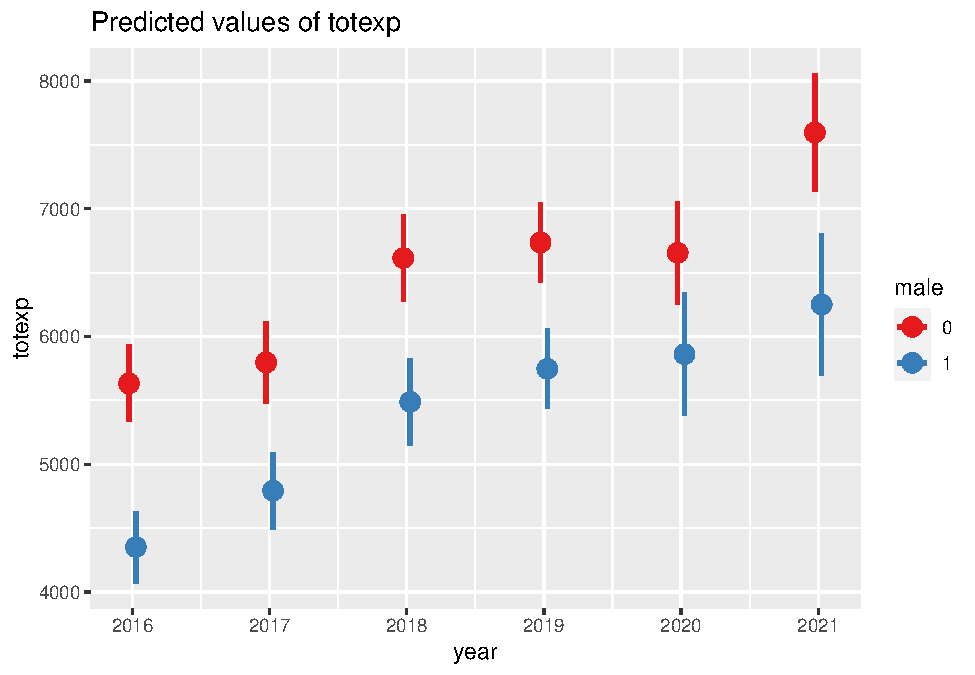
\includegraphics{_main_files/figure-latex/unnamed-chunk-76-1.pdf}

We could also plot the average marginal effects using \texttt{ggplot2} with the \texttt{ggpredict} package.

\begin{Shaded}
\begin{Highlighting}[]
\CommentTok{\# Plot the predicted values}
\NormalTok{fit.dataframe }\OtherTok{\textless{}{-}} \FunctionTok{ggpredict}\NormalTok{(survey\_model, }\AttributeTok{terms =} \FunctionTok{c}\NormalTok{(}\StringTok{"year"}\NormalTok{, }\StringTok{"male"}\NormalTok{), }\AttributeTok{design =}\NormalTok{ survey\_design)}
\FunctionTok{ggplot}\NormalTok{(fit.dataframe, }\FunctionTok{aes}\NormalTok{(x, predicted, }\AttributeTok{colour =}\NormalTok{ group)) }\SpecialCharTok{+}
  \FunctionTok{geom\_line}\NormalTok{(}\AttributeTok{size =} \FloatTok{1.5}\NormalTok{) }\SpecialCharTok{+}
  \FunctionTok{geom\_point}\NormalTok{(}\AttributeTok{size =} \DecValTok{5}\NormalTok{) }\SpecialCharTok{+} 
  \FunctionTok{labs}\NormalTok{(}
    \AttributeTok{x =} \StringTok{"Year"}\NormalTok{,}
    \AttributeTok{y =} \StringTok{"Total healthcare costs"}\NormalTok{,}
    \AttributeTok{colour =} \FunctionTok{get\_legend\_title}\NormalTok{(fit.dataframe)}
\NormalTok{  )}
\end{Highlighting}
\end{Shaded}

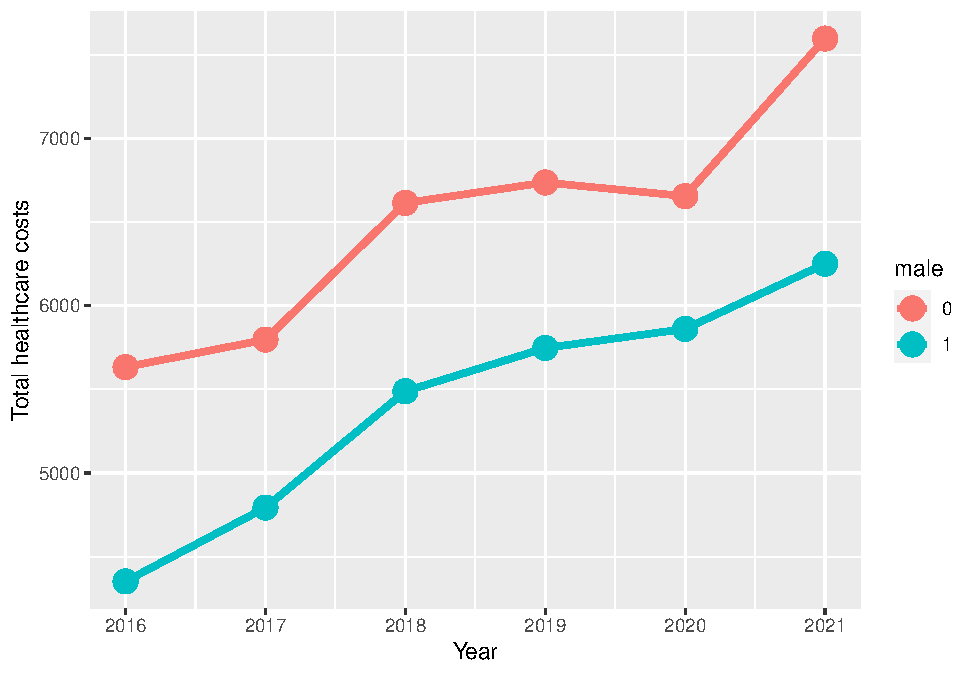
\includegraphics{_main_files/figure-latex/unnamed-chunk-77-1.pdf}

There are a few important things to plot with these figures.

In the first figure below, we see that the slopes or change in average total healthcare costs across the years are displayed for the males and females. The output from the \texttt{margins} function provides us with the within group change in total healthcare costs for males and females across time. For instance, the change from 2016 to 2017 for females (which is also called the slope between 2016 and 2017) was \$165. For males, their slope was \$441.

\begin{figure}
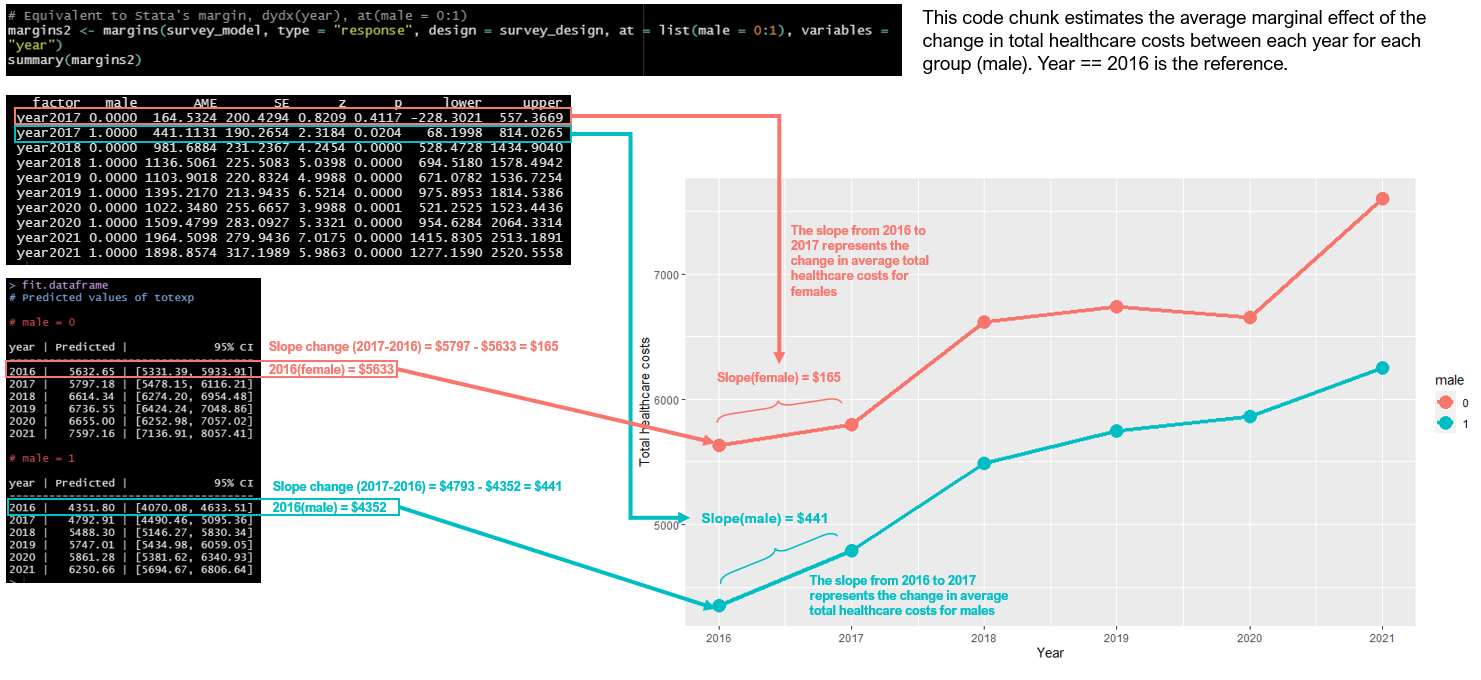
\includegraphics[width=1\linewidth]{Figure 5_2} \caption{Average marginal effects or the Slopes of males and females.}\label{fig:unnamed-chunk-78}
\end{figure}

In the second figure, we can use the output from the \texttt{margins1} object to estimate the difference in total healthcare costs at each year between males and females. For instance, we can visualize the difference in total healthcare costs at 2019 between males and females is -\$990.

\begin{figure}
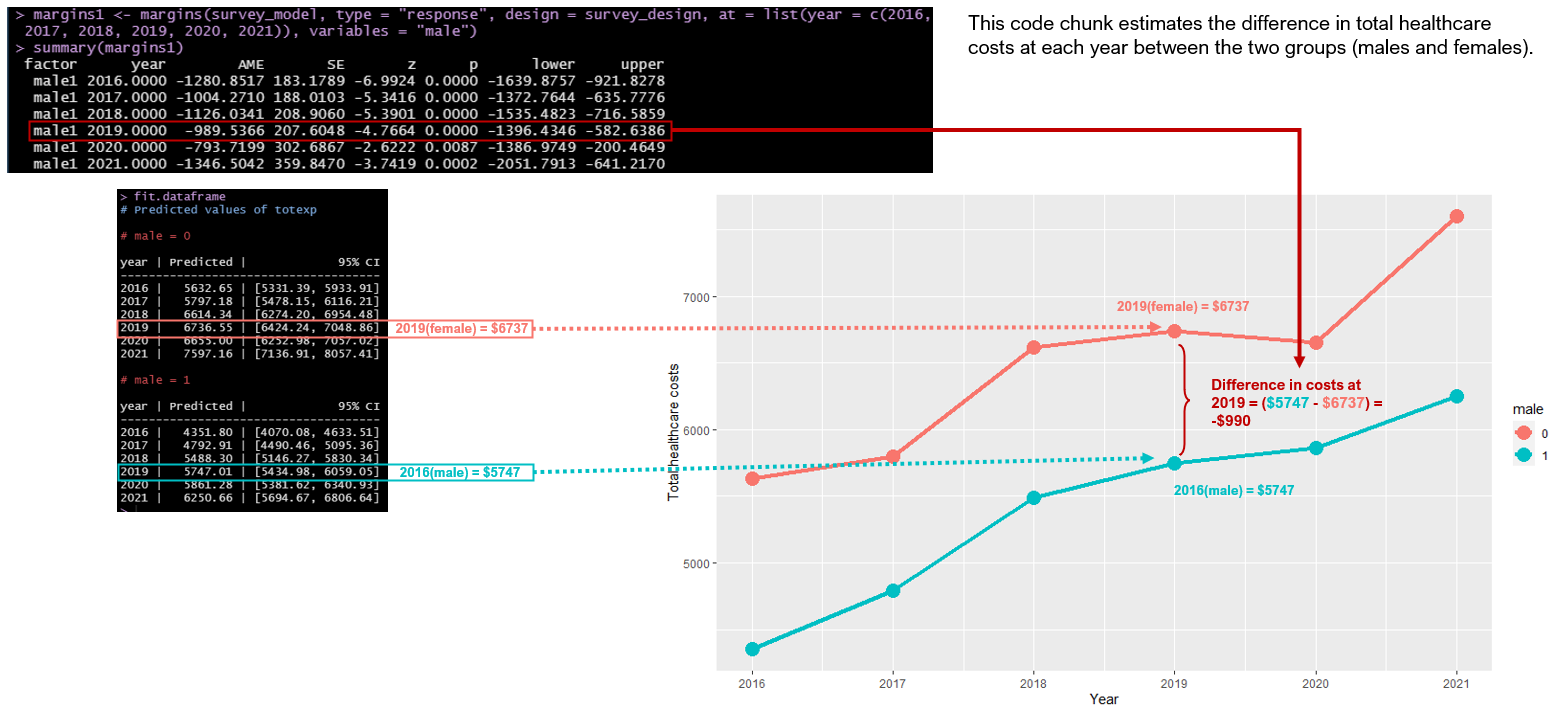
\includegraphics[width=1\linewidth]{Figure 5_3} \caption{Differences in total healthcare costs between males and females in 2019.}\label{fig:unnamed-chunk-79}
\end{figure}

The last figure is the most important. This visualizes the interaction term results. We are mostly interested in the interaction terms for trend analysis. The interaction terms tell us the differences in the total healthcare costs between males and females as the year changes (2016 to 2018).

For instance, the slope change for females between 2018 and 2016 was approximately \$981. The slope change for males between 2018 and 2016 was \$1136. The difference between these two slope changes for males and females is \$1136 - \$981 = \$155. This is our difference in the changes estimation, or we can state that this is the differences in total healthcare costs between males and females as the year changed from 2016 to 2018. But, this was not statistically significant since the 95\% CI includes zero (95\% CI: -\$391, \$701).

\begin{figure}
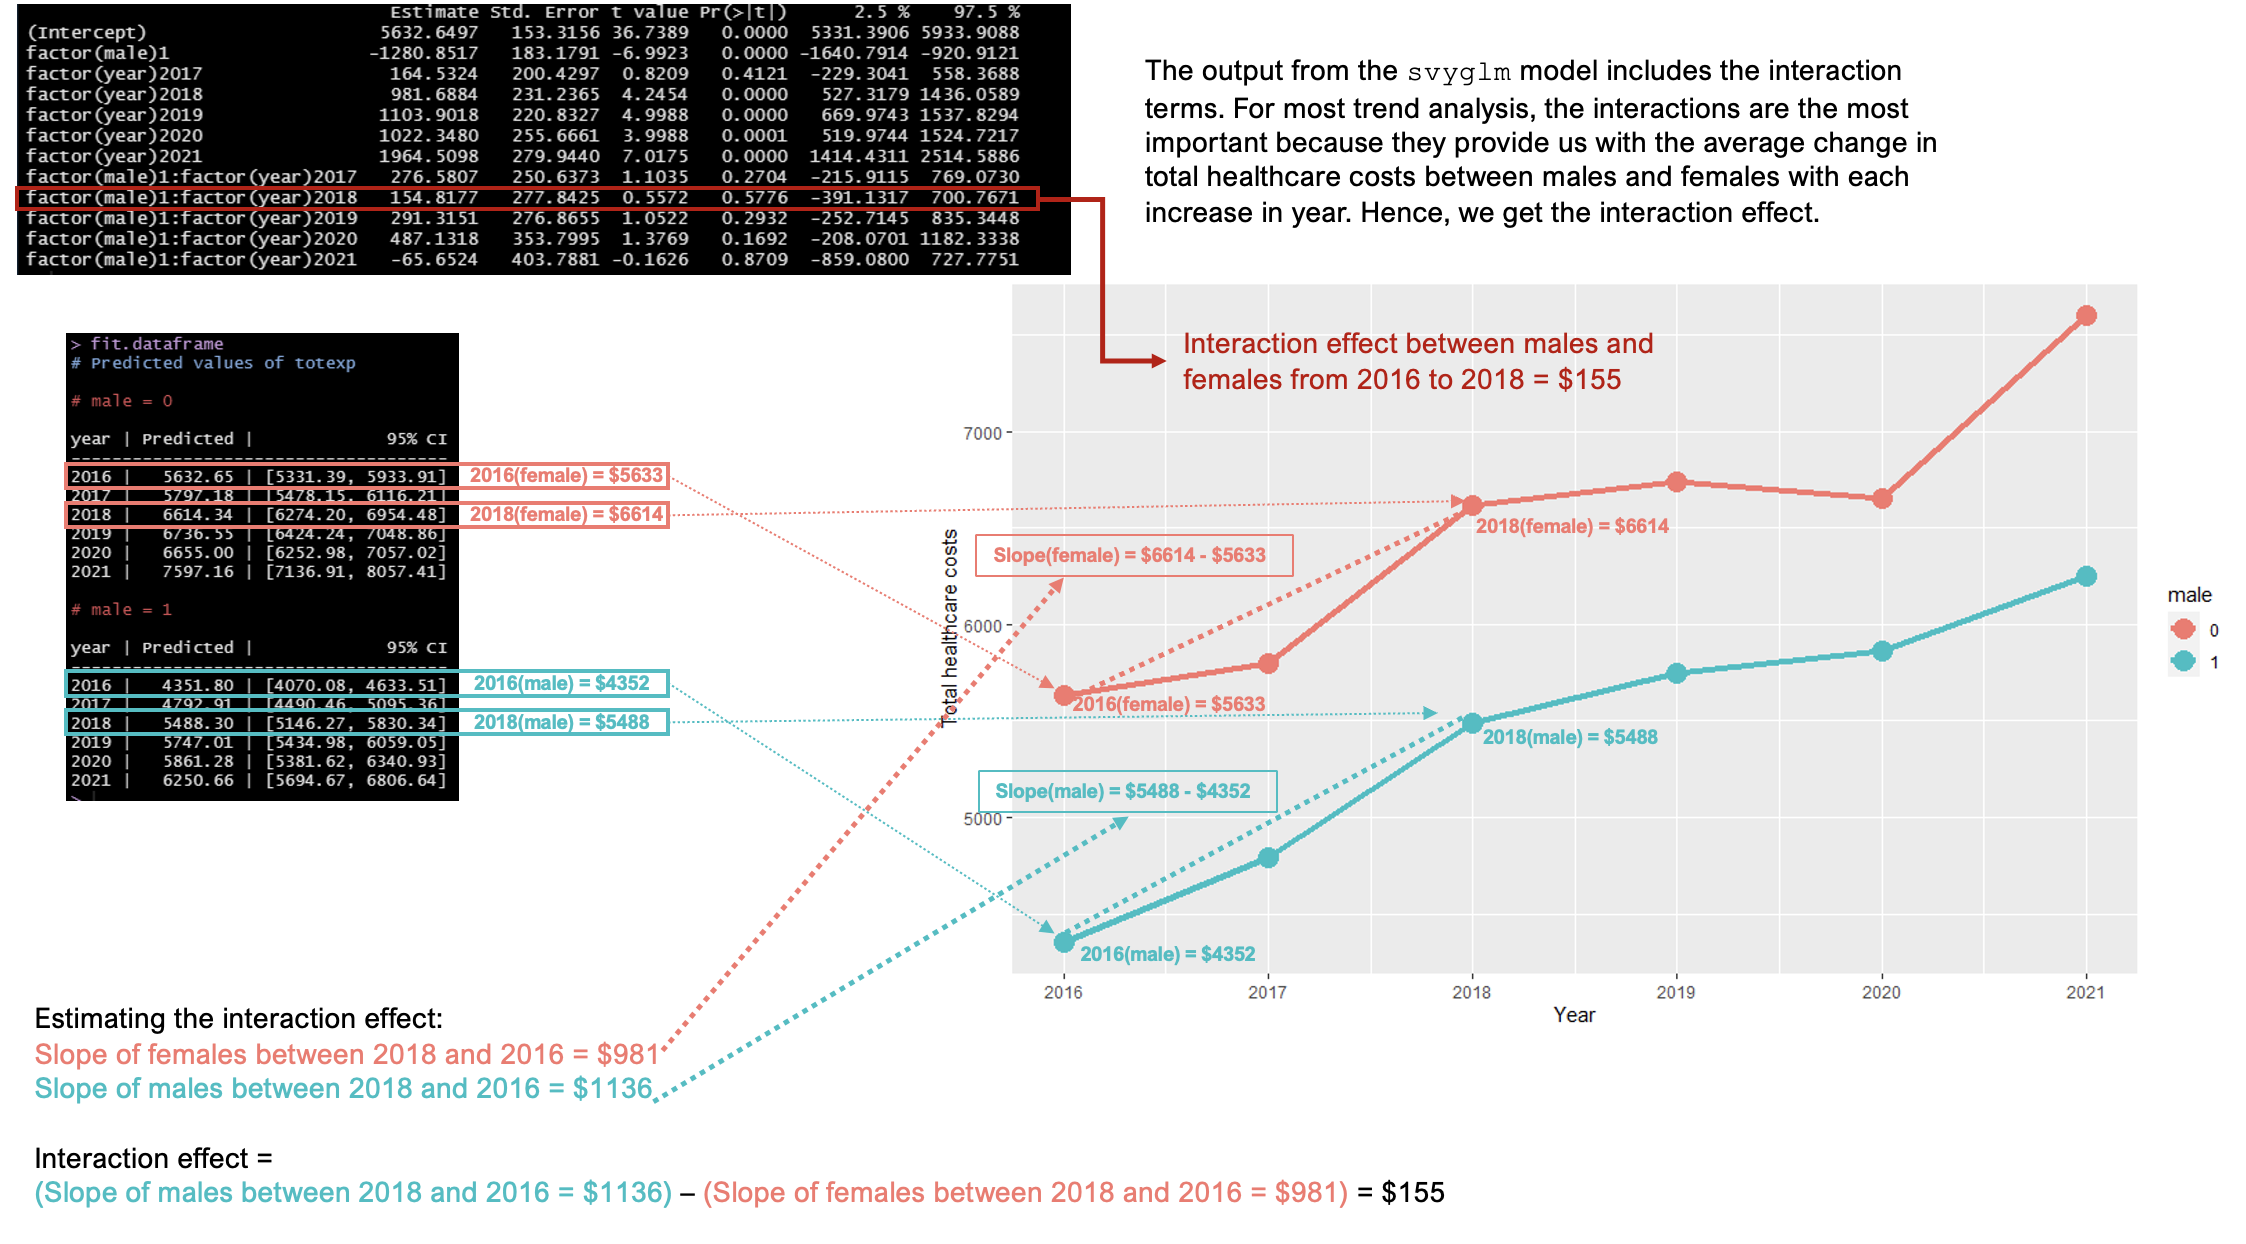
\includegraphics[width=1\linewidth]{Figure 5_4} \caption{Interaction terms - difference in the changes between males and females when year increased from 2016 to 2018.}\label{fig:unnamed-chunk-80}
\end{figure}

\hypertarget{conclusions-4}{%
\section{Conclusions}\label{conclusions-4}}

Trend analysis can be performed using linear models. The ease of interpretation and simple execution makes this ideal for most stakeholders. Moreover, the \texttt{svyglm} function allows us to incorporate the survey weights from the complex survey design of MEPS to generate standard errors that were representative of the general U.S. population. Although the \texttt{margins} package is helpful in estimating the average marginal effects, there are other alternatives such as the \href{https://github.com/vincentarelbundock/marginaleffects}{\texttt{marginaleffects} package}.

Additionally, more complex models exist that account for autoregressive correlations and more precise estimations of the variance. However, they are harder to implement with complex survey designs. Unfortunately, I have not been able to figure out how to perform some of these more complex longitudinal data analysis with alternative models (e.g., linear mixed effects models) that incorporate the survey weights. For these scenarios, I prefer to use \texttt{Stata}, which makes it convenient to apply survey weights in more complex models. Perhaps, I'll create some tutorials using \texttt{Stata} for these more complex longitudinal models in the future.

\hypertarget{acknowledgements-4}{%
\section{Acknowledgements}\label{acknowledgements-4}}

I am grateful to the author of the \texttt{margins} package, Thomas J. Leeper. You can find his \texttt{margins} package on his \href{https://github.com/leeper/margins}{\texttt{GitHub\ site}}.

Additionally, the \texttt{marginaleffects} package by Vincent Arel-Bundock has helped me to compare some of \texttt{R}'s marginal effects commands with \texttt{Stata}. You can find his GitHub site \href{https://github.com/vincentarelbundock/marginaleffects}{here}.

\hypertarget{work-in-progress-1}{%
\section{Work in progress}\label{work-in-progress-1}}

This is a work in progress so expect some updates in the future.

\hypertarget{disclaimers-1}{%
\section{Disclaimers}\label{disclaimers-1}}

Any errors or mistakes are those of the author.

This is only for educational purposes.

This was built under R version 4.2.2 ``Innocent and Trusting''

\hypertarget{itsa}{%
\chapter{Interrupted time series analysis (ITSA) with R: A short tutorial}\label{itsa}}

\hypertarget{introduction-5}{%
\section{Introduction}\label{introduction-5}}

Previously, I wrote a tutorial on how to perform an interrupted time series analysis (ITSA) in \texttt{Stata}, which is located on my RPubs site (\href{https://rpubs.com/mbounthavong/itsa_stata}{link}). This had me thinking of how to perform an ITSA using \texttt{R}. So, I decided to create a short tutorial on how to perform an ITSA on \texttt{R} using the \href{https://meps.ahrq.gov/mepsweb/}{Agency for Healthcare Research and Quality (AHRQ) Medical Expenditure Panel Survey (MEPS)} dataset. I tried several ways to do this, and I think I've found a nice approach that leverages survey weights from the MEPS database. Although I'm writing this ITSA tutorial with this approach, I plan on researching other methods to perform an ITSA in \texttt{R} so stay tuned.

This short tutorial will summarize how to perform an ITSA using a linear regression model with survey weights applied from the MEPS database. (Note: I previously wrote a tutorial on how to apply weights from MEPS data (\href{https://rpubs.com/mbounthavong/MEPS_tutorial_3_applying_weights}{link}).

\hypertarget{motivating-example---total-healthcare-costs-from-2016-to-2021-by-sex}{%
\section{Motivating example - Total Healthcare Costs from 2016 to 2021 by sex}\label{motivating-example---total-healthcare-costs-from-2016-to-2021-by-sex}}

We'll use the MEPS database to compare the trends in total healthcare costs between sex. We'll assume that a policy or intervention was implemented in 2019, which may have changed the healthcare costs levels and trends between males and females.

I pooled data from 2016 to 2021 and adjusted the weights. I won't go into details on how to create this dataset for this tutorial since I provided a detailed summary in a previous tutorial. For more details on how I created this dataset, please refer to my previous tutorial (\href{https://rpubs.com/mbounthavong/MEPS_tutorial_5_simple_trend_analysis}{link}).

\begin{Shaded}
\begin{Highlighting}[]
\CommentTok{\# To install MEPS package in R, you need to do a couple of things.}
\DocumentationTok{\#\#\# Step 1: Install the "devtools" package. }
\CommentTok{\#install.packages("devtools")}

\DocumentationTok{\#\#\# Step 2: Install the "MEPS" package from the AHRQ MEPS GitHub site. }
\CommentTok{\#devtools::install\_github("e{-}mitchell/meps\_r\_pkg/MEPS")}

\DocumentationTok{\#\#\# step 3: Load the MEPS package}
\FunctionTok{library}\NormalTok{(}\StringTok{"MEPS"}\NormalTok{) }\DocumentationTok{\#\# You need to load the library every time you restart R}

\DocumentationTok{\#\#\# Step 4: Load the other libraries}
\FunctionTok{library}\NormalTok{(}\StringTok{"survey"}\NormalTok{)}
\FunctionTok{library}\NormalTok{(}\StringTok{"foreign"}\NormalTok{)}
\FunctionTok{library}\NormalTok{(}\StringTok{"dplyr"}\NormalTok{)}
\FunctionTok{library}\NormalTok{(}\StringTok{"ggplot2"}\NormalTok{)}
\FunctionTok{library}\NormalTok{(}\StringTok{"questionr"}\NormalTok{) }\CommentTok{\# remotes::install\_github("juba/questionr")}
\FunctionTok{library}\NormalTok{(}\StringTok{"lspline"}\NormalTok{)  }\CommentTok{\# devtools::install\_github("mbojan/lspline", build\_vignettes=TRUE)}
\FunctionTok{library}\NormalTok{(}\StringTok{"ggeffects"}\NormalTok{) }\CommentTok{\# remotes::install\_github("strengejacke/ggeffects")}
\FunctionTok{library}\NormalTok{(}\StringTok{"margins"}\NormalTok{)}


\CommentTok{\# There are two ways to load data from AHRQ MEPS website:}
\DocumentationTok{\#\#\#\# Method 1: Load data from AHRQ MEPS website}
\NormalTok{hc2021 }\OtherTok{=} \FunctionTok{read\_MEPS}\NormalTok{(}\AttributeTok{file =} \StringTok{"h233"}\NormalTok{)}
\NormalTok{hc2020 }\OtherTok{=} \FunctionTok{read\_MEPS}\NormalTok{(}\AttributeTok{file =} \StringTok{"h224"}\NormalTok{)}
\NormalTok{hc2019 }\OtherTok{=} \FunctionTok{read\_MEPS}\NormalTok{(}\AttributeTok{file =} \StringTok{"h216"}\NormalTok{)}
\NormalTok{hc2018 }\OtherTok{=} \FunctionTok{read\_MEPS}\NormalTok{(}\AttributeTok{file =} \StringTok{"h209"}\NormalTok{)}
\NormalTok{hc2017 }\OtherTok{=} \FunctionTok{read\_MEPS}\NormalTok{(}\AttributeTok{file =} \StringTok{"h201"}\NormalTok{)}
\NormalTok{hc2016 }\OtherTok{=} \FunctionTok{read\_MEPS}\NormalTok{(}\AttributeTok{file =} \StringTok{"h192"}\NormalTok{)}


\DocumentationTok{\#\#\#\# Method 2: Load data from AHRQ MEPS website}
\NormalTok{hc2021 }\OtherTok{=} \FunctionTok{read\_MEPS}\NormalTok{(}\AttributeTok{year =} \DecValTok{2021}\NormalTok{, }\AttributeTok{type =} \StringTok{"FYC"}\NormalTok{)}
\NormalTok{hc2020 }\OtherTok{=} \FunctionTok{read\_MEPS}\NormalTok{(}\AttributeTok{year =} \DecValTok{2020}\NormalTok{, }\AttributeTok{type =} \StringTok{"FYC"}\NormalTok{)}
\NormalTok{hc2019 }\OtherTok{=} \FunctionTok{read\_MEPS}\NormalTok{(}\AttributeTok{year =} \DecValTok{2019}\NormalTok{, }\AttributeTok{type =} \StringTok{"FYC"}\NormalTok{)}
\NormalTok{hc2018 }\OtherTok{=} \FunctionTok{read\_MEPS}\NormalTok{(}\AttributeTok{year =} \DecValTok{2018}\NormalTok{, }\AttributeTok{type =} \StringTok{"FYC"}\NormalTok{)}
\NormalTok{hc2017 }\OtherTok{=} \FunctionTok{read\_MEPS}\NormalTok{(}\AttributeTok{year =} \DecValTok{2017}\NormalTok{, }\AttributeTok{type =} \StringTok{"FYC"}\NormalTok{)}
\NormalTok{hc2016 }\OtherTok{=} \FunctionTok{read\_MEPS}\NormalTok{(}\AttributeTok{year =} \DecValTok{2016}\NormalTok{, }\AttributeTok{type =} \StringTok{"FYC"}\NormalTok{)}


\DocumentationTok{\#\# Change column names to lowercase}
\FunctionTok{names}\NormalTok{(hc2021) }\OtherTok{\textless{}{-}} \FunctionTok{tolower}\NormalTok{(}\FunctionTok{names}\NormalTok{(hc2021))}
\FunctionTok{names}\NormalTok{(hc2020) }\OtherTok{\textless{}{-}} \FunctionTok{tolower}\NormalTok{(}\FunctionTok{names}\NormalTok{(hc2020))}
\FunctionTok{names}\NormalTok{(hc2019) }\OtherTok{\textless{}{-}} \FunctionTok{tolower}\NormalTok{(}\FunctionTok{names}\NormalTok{(hc2019))}
\FunctionTok{names}\NormalTok{(hc2018) }\OtherTok{\textless{}{-}} \FunctionTok{tolower}\NormalTok{(}\FunctionTok{names}\NormalTok{(hc2018))}
\FunctionTok{names}\NormalTok{(hc2017) }\OtherTok{\textless{}{-}} \FunctionTok{tolower}\NormalTok{(}\FunctionTok{names}\NormalTok{(hc2017))}
\FunctionTok{names}\NormalTok{(hc2016) }\OtherTok{\textless{}{-}} \FunctionTok{tolower}\NormalTok{(}\FunctionTok{names}\NormalTok{(hc2016))}


\CommentTok{\# We need the linkage file with the appropriate stratum of the primary sampling unit (STRA9621) and primary sampling unit (PSU9621). (Note: Each year, the linkage file sampling unit name changes)}
\NormalTok{linkage }\OtherTok{=} \FunctionTok{read\_MEPS}\NormalTok{(}\AttributeTok{type =} \StringTok{"Pooled linkage"}\NormalTok{) }
\FunctionTok{names}\NormalTok{(linkage) }\OtherTok{\textless{}{-}} \FunctionTok{tolower}\NormalTok{(}\FunctionTok{names}\NormalTok{(linkage)) }\CommentTok{\# change variable name to lower case}



\CommentTok{\# Select specific variables}

\DocumentationTok{\#\#\# 2021}
\NormalTok{hc2021p }\OtherTok{=}\NormalTok{ hc2021 }\SpecialCharTok{\%\textgreater{}\%}
  \FunctionTok{rename}\NormalTok{(}
    \AttributeTok{perwt =}\NormalTok{ perwt21f,}
    \AttributeTok{totexp =}\NormalTok{ totexp21,}
    \AttributeTok{ertexp =}\NormalTok{ ertexp21) }\SpecialCharTok{\%\textgreater{}\%}
  \FunctionTok{select}\NormalTok{(}
\NormalTok{    dupersid, }
\NormalTok{    panel, }
\NormalTok{    varstr, }
\NormalTok{    varpsu,}
\NormalTok{    perwt,}
\NormalTok{    sex,}
\NormalTok{    totexp,}
\NormalTok{    ertexp)}
\NormalTok{hc2021p}\SpecialCharTok{$}\NormalTok{year }\OtherTok{\textless{}{-}} \DecValTok{2021}

\DocumentationTok{\#\#\# 2020}
\NormalTok{hc2020p }\OtherTok{=}\NormalTok{ hc2020 }\SpecialCharTok{\%\textgreater{}\%}
  \FunctionTok{rename}\NormalTok{(}
    \AttributeTok{perwt =}\NormalTok{ perwt20f,}
    \AttributeTok{totexp =}\NormalTok{ totexp20,}
    \AttributeTok{ertexp =}\NormalTok{ ertexp20) }\SpecialCharTok{\%\textgreater{}\%}
  \FunctionTok{select}\NormalTok{(}
\NormalTok{    dupersid, }
\NormalTok{    panel, }
\NormalTok{    varstr, }
\NormalTok{    varpsu,}
\NormalTok{    perwt,}
\NormalTok{    sex,}
\NormalTok{    totexp,}
\NormalTok{    ertexp)}
\NormalTok{hc2020p}\SpecialCharTok{$}\NormalTok{year }\OtherTok{\textless{}{-}} \DecValTok{2020}


\DocumentationTok{\#\#\# 2019}
\NormalTok{hc2019p }\OtherTok{=}\NormalTok{ hc2019 }\SpecialCharTok{\%\textgreater{}\%}
  \FunctionTok{rename}\NormalTok{(}
    \AttributeTok{perwt =}\NormalTok{ perwt19f,}
    \AttributeTok{totexp =}\NormalTok{ totexp19,}
    \AttributeTok{ertexp =}\NormalTok{ ertexp19) }\SpecialCharTok{\%\textgreater{}\%}
  \FunctionTok{select}\NormalTok{(}
\NormalTok{    dupersid, }
\NormalTok{    panel, }
\NormalTok{    varstr, }
\NormalTok{    varpsu,}
\NormalTok{    perwt,}
\NormalTok{    sex,}
\NormalTok{    totexp,}
\NormalTok{    ertexp)}
\NormalTok{hc2019p}\SpecialCharTok{$}\NormalTok{year }\OtherTok{\textless{}{-}} \DecValTok{2019}

\DocumentationTok{\#\#\# 2018}
\NormalTok{hc2018p }\OtherTok{=}\NormalTok{ hc2018 }\SpecialCharTok{\%\textgreater{}\%}
  \FunctionTok{rename}\NormalTok{(}
    \AttributeTok{perwt =}\NormalTok{ perwt18f,}
    \AttributeTok{totexp =}\NormalTok{ totexp18,}
    \AttributeTok{ertexp =}\NormalTok{ ertexp18) }\SpecialCharTok{\%\textgreater{}\%}
  \FunctionTok{select}\NormalTok{(}
\NormalTok{    dupersid, }
\NormalTok{    panel, }
\NormalTok{    varstr, }
\NormalTok{    varpsu,}
\NormalTok{    perwt,}
\NormalTok{    sex,}
\NormalTok{    totexp,}
\NormalTok{    ertexp)}
\NormalTok{hc2018p}\SpecialCharTok{$}\NormalTok{year }\OtherTok{\textless{}{-}} \DecValTok{2018}

\DocumentationTok{\#\#\# 2017}
\NormalTok{hc2017p }\OtherTok{=}\NormalTok{ hc2017 }\SpecialCharTok{\%\textgreater{}\%}
  \FunctionTok{rename}\NormalTok{(}
    \AttributeTok{perwt =}\NormalTok{ perwt17f,}
    \AttributeTok{totexp =}\NormalTok{ totexp17,}
    \AttributeTok{ertexp =}\NormalTok{ ertexp17) }\SpecialCharTok{\%\textgreater{}\%}
  \FunctionTok{select}\NormalTok{(}
\NormalTok{    dupersid, }
\NormalTok{    panel, }
\NormalTok{    varstr, }
\NormalTok{    varpsu,}
\NormalTok{    perwt,}
\NormalTok{    sex,}
\NormalTok{    totexp,}
\NormalTok{    ertexp)}
\NormalTok{hc2017p}\SpecialCharTok{$}\NormalTok{year }\OtherTok{\textless{}{-}} \DecValTok{2017}

\DocumentationTok{\#\#\# 2016}
\NormalTok{hc2016p }\OtherTok{=}\NormalTok{ hc2016 }\SpecialCharTok{\%\textgreater{}\%}
  \FunctionTok{rename}\NormalTok{(}
    \AttributeTok{perwt =}\NormalTok{ perwt16f,}
    \AttributeTok{totexp =}\NormalTok{ totexp16,}
    \AttributeTok{ertexp =}\NormalTok{ ertexp16) }\SpecialCharTok{\%\textgreater{}\%}
  \FunctionTok{select}\NormalTok{(}
\NormalTok{    dupersid, }
\NormalTok{    panel, }
\NormalTok{    varstr, }
\NormalTok{    varpsu,}
\NormalTok{    perwt,}
\NormalTok{    sex,}
\NormalTok{    totexp,}
\NormalTok{    ertexp)}
\NormalTok{hc2016p}\SpecialCharTok{$}\NormalTok{year }\OtherTok{\textless{}{-}} \DecValTok{2016}


\CommentTok{\# Merge data and adjust the person weight by 6 years}
\NormalTok{pool\_data }\OtherTok{=} \FunctionTok{bind\_rows}\NormalTok{(hc2021p, }
\NormalTok{                      hc2020p,}
\NormalTok{                      hc2019p,}
\NormalTok{                      hc2018p,}
\NormalTok{                      hc2017p,}
\NormalTok{                      hc2016p) }\SpecialCharTok{\%\textgreater{}\%}
  \FunctionTok{mutate}\NormalTok{(}\AttributeTok{poolwt =}\NormalTok{ perwt }\SpecialCharTok{/} \DecValTok{6}\NormalTok{)}


\CommentTok{\# Add a new variable for the pre{-}post index year at 2019}
\NormalTok{pool\_data}\SpecialCharTok{$}\NormalTok{period[pool\_data}\SpecialCharTok{$}\NormalTok{year }\SpecialCharTok{\textgreater{}=} \DecValTok{2016} \SpecialCharTok{\&}\NormalTok{ pool\_data}\SpecialCharTok{$}\NormalTok{year }\SpecialCharTok{\textless{}} \DecValTok{2019}\NormalTok{] }\OtherTok{=} \DecValTok{0}
\NormalTok{pool\_data}\SpecialCharTok{$}\NormalTok{period[pool\_data}\SpecialCharTok{$}\NormalTok{year }\SpecialCharTok{\textgreater{}=} \DecValTok{2019} \SpecialCharTok{\&}\NormalTok{ pool\_data}\SpecialCharTok{$}\NormalTok{year }\SpecialCharTok{\textless{}} \DecValTok{2022}\NormalTok{] }\OtherTok{=} \DecValTok{1}
\FunctionTok{head}\NormalTok{(pool\_data)}
\end{Highlighting}
\end{Shaded}

\begin{verbatim}
## # A tibble: 6 x 11
##   dupersid   panel            varstr varpsu perwt sex          totexp ertexp
##   <chr>      <dbl+lbl>         <dbl>  <dbl> <dbl> <dbl+lbl>     <dbl>  <dbl>
## 1 2320005101 23 [23 PANEL 23]   2079      1 6785. 2 [2 FEMALE]   4908      0
## 2 2320005102 23 [23 PANEL 23]   2079      1 6177. 1 [1 MALE]    21257      0
## 3 2320006101 23 [23 PANEL 23]   2028      1 1599. 2 [2 FEMALE]    827      0
## 4 2320006102 23 [23 PANEL 23]   2028      1 1649. 1 [1 MALE]        0      0
## 5 2320006103 23 [23 PANEL 23]   2028      1 2892. 1 [1 MALE]        0      0
## 6 2320012102 23 [23 PANEL 23]   2069      2 1273. 2 [2 FEMALE]   9813      0
##    year poolwt period
##   <dbl>  <dbl>  <dbl>
## 1  2021  1131.      1
## 2  2021  1029.      1
## 3  2021   267.      1
## 4  2021   275.      1
## 5  2021   482.      1
## 6  2021   212.      1
\end{verbatim}

\begin{Shaded}
\begin{Highlighting}[]
\CommentTok{\# Reduce the linkage file to only include dupersid, panel, stra9621, psu9621}
\NormalTok{linkage\_file }\OtherTok{=}\NormalTok{ linkage }\SpecialCharTok{\%\textgreater{}\%}
  \FunctionTok{select}\NormalTok{(dupersid, panel, stra9621, psu9621)}

\CommentTok{\# Merge link file with main data}
\NormalTok{pool\_data\_linked }\OtherTok{=} \FunctionTok{left\_join}\NormalTok{(pool\_data,}
\NormalTok{                             linkage\_file, }
                             \AttributeTok{by =} \FunctionTok{c}\NormalTok{(}\StringTok{"dupersid"}\NormalTok{, }\StringTok{"panel"}\NormalTok{))}
\end{Highlighting}
\end{Shaded}

\hypertarget{interrupted-time-series-analysis-design}{%
\section{Interrupted Time Series Analysis Design}\label{interrupted-time-series-analysis-design}}

In this ITSA motivating example, we are going to compare the trends in healthcare total costs between males and females before and after the hypothetical policy intervention, which was implemented in 2019. The ITSA design is illustrated in the figure below.

For this example, the ITSA model is denoted by the following:

\(Y_i = \beta_0 + \beta_1(T_i) + \beta_2(X_i) + \beta_3(T_i * X_i) + \beta_4(Sex_i) + \beta_5(Sex_i * T_i) + \beta_6(Sex_i * X_i) + \beta_7(Sex_i * T_i * X_i) + \epsilon_i\),

where \(Sex_i\) is a new variable that denotes the groups (e.g., sexes), \(\beta_4\) denotes the difference in the outcomes between the groups (e.g., sexes) at beginning of the study (\(T = 0\)), \(\beta_5\) denotes the difference in the slopes between the groups before the intervention, \(\beta_6\) denotes the difference in the level changes between the groups immediately after implementation of the intervention \(X\), and \(\beta_7\) denotes the difference in the slopes after and before the intervention between the groups (e.g., difference-in-differences).

\begin{figure}
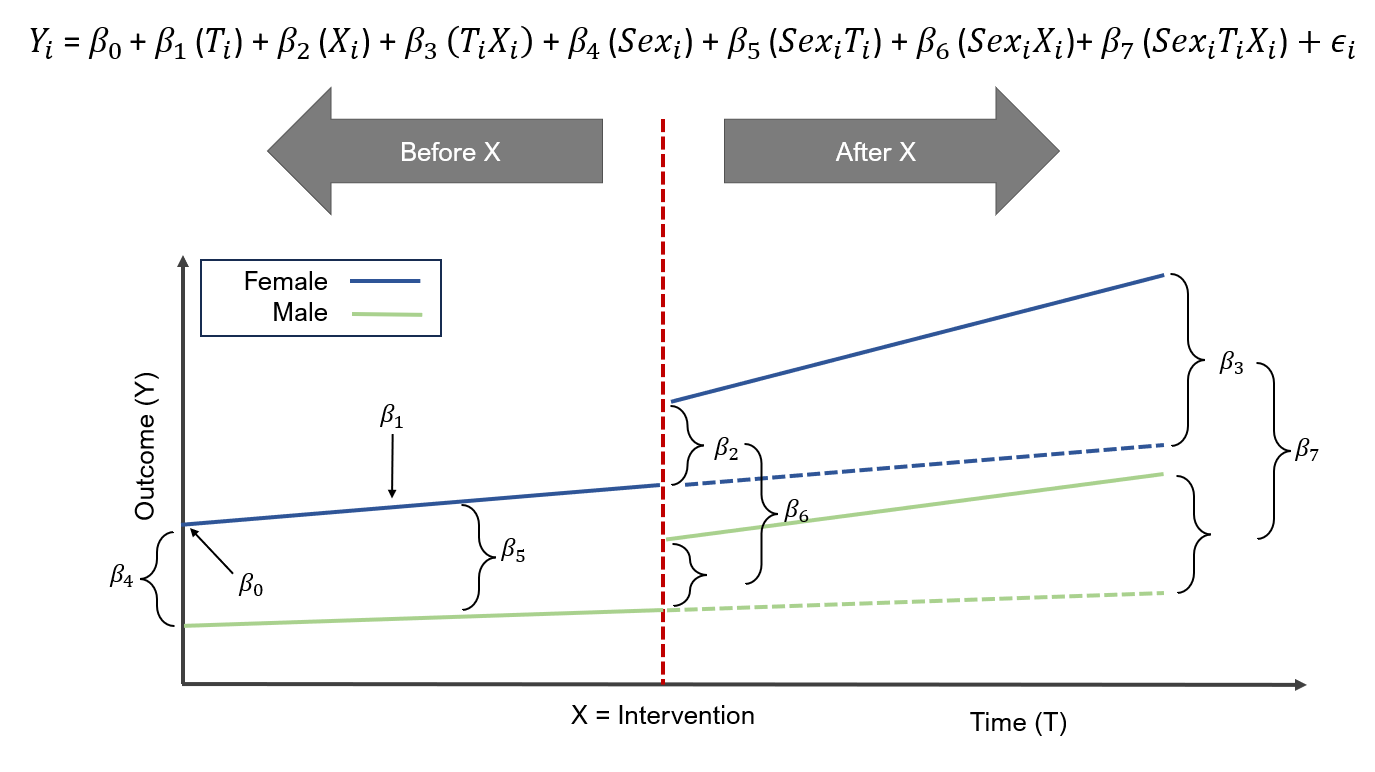
\includegraphics[width=1\linewidth]{Figure 6_1} \caption{ITSA for two groups (`sex`) before and after the intervention (`X`).}\label{fig:unnamed-chunk-82}
\end{figure}

\hypertarget{set-up-the-survey-options}{%
\section{Set up the survey options}\label{set-up-the-survey-options}}

In order to estimate the appropriate costs and standard errors, we will need to set up the survey options and survey design using the weights from MEPS. We will use the \texttt{svydesign} function to load the primary sampling unit, individual weights, and strata, which we will then assign to an object called \texttt{survey\_design}. Please see the code below:

\begin{Shaded}
\begin{Highlighting}[]
\CommentTok{\# Set the survey options}
\FunctionTok{options}\NormalTok{(}\AttributeTok{survey.lonely.psu =} \StringTok{"adjust"}\NormalTok{)}
\FunctionTok{options}\NormalTok{(}\AttributeTok{survey.adjust.domain.lonely =} \ConstantTok{TRUE}\NormalTok{)}


\CommentTok{\# Define the survey design}
\NormalTok{survey\_design }\OtherTok{=} \FunctionTok{svydesign}\NormalTok{(}
                          \AttributeTok{id =} \SpecialCharTok{\textasciitilde{}}\NormalTok{psu9621,}
                          \AttributeTok{strata =} \SpecialCharTok{\textasciitilde{}}\NormalTok{stra9621,}
                          \AttributeTok{weights =} \SpecialCharTok{\textasciitilde{}}\NormalTok{poolwt,}
                          \AttributeTok{data =}\NormalTok{ pool\_data\_linked,}
                          \AttributeTok{nest =} \ConstantTok{TRUE}\NormalTok{)}
\end{Highlighting}
\end{Shaded}

\hypertarget{descriptive-analysis}{%
\section{Descriptive analysis}\label{descriptive-analysis}}

Once that's done, we can do some descriptive analysis.

Using the \texttt{svytable} function, we can estimate the weighted-sample of males and females in the United States (US). In our MEPS dataset, there are 160,228,773 males and 166,678,038 females, which is representative of the non-institutionalized civilian US population.

\begin{Shaded}
\begin{Highlighting}[]
\FunctionTok{svytable}\NormalTok{(}\SpecialCharTok{\textasciitilde{}}\NormalTok{sex, }\AttributeTok{design =}\NormalTok{ survey\_design)}
\end{Highlighting}
\end{Shaded}

\begin{verbatim}
## sex
##           1           2 
## 160228772.9 166678038.1
\end{verbatim}

Moreover, we can look at the survey-weighted total healthcare costs between males and females. For instance, in 2016, the average annual total healthcare costs for males and females were \$4351 and \$5633 per person, respectively.

\begin{Shaded}
\begin{Highlighting}[]
\NormalTok{df1 }\OtherTok{\textless{}{-}} \FunctionTok{svyby}\NormalTok{(}\SpecialCharTok{\textasciitilde{}}\NormalTok{totexp, }\SpecialCharTok{\textasciitilde{}}\NormalTok{year}\SpecialCharTok{+}\NormalTok{sex, survey\_design, svymean)}
\NormalTok{df1}
\end{Highlighting}
\end{Shaded}

\begin{verbatim}
##        year sex      totexp          se
## 2016.1 2016   1 4351.797969 143.3686740
## 2017.1 2017   1 4792.911089 153.9208333
## 2018.1 2018   1 5488.304037 174.0676798
## 2019.1 2019   1 5747.014931 158.7998588
## 2020.1 2020   1 5861.277852 244.1047619
## 2021.1 2021   1 6250.655387 282.9494481
## 2016.2 2016   2 5632.649717 153.3156133
## 2017.2 2017   2 5797.182100 162.3600394
## 2018.2 2018   2 6614.338104 173.1029815
## 2019.2 2019   2 6736.551546 158.9384299
## 2020.2 2020   2 6654.997756 204.6000543
## 2021.2 2021   2 7597.159563 234.2313172
\end{verbatim}

We can also look at the survey-weighted average cost before and after the intervention (before and after 2019). For instance, before the intervention the survey-weighted average total healthcare cost for males and females were \$4880 and \$6016, respectively. After the intervention, the survey-weighted average total healthcare costs for males and females were \$5954 and \$6997, respectively.

\begin{Shaded}
\begin{Highlighting}[]
\NormalTok{df2 }\OtherTok{\textless{}{-}} \FunctionTok{svyby}\NormalTok{(}\SpecialCharTok{\textasciitilde{}}\NormalTok{totexp, }\SpecialCharTok{\textasciitilde{}}\NormalTok{sex}\SpecialCharTok{+}\NormalTok{period, survey\_design, svymean)}
\NormalTok{df2}
\end{Highlighting}
\end{Shaded}

\begin{verbatim}
##     sex period      totexp          se
## 1.0   1      0 4879.518399 103.6333733
## 2.0   2      0 6016.325527 109.4863008
## 1.1   1      1 5954.493236 166.0967456
## 2.1   2      1 6997.285661 138.6561924
\end{verbatim}

We can visualize the trend of the survey-weighted total healthcare costs for males and females from 2016 to 2021 using the \texttt{ggsurvey} function. From the plot, we can see that the female group had a higher total healthcare cost trend compared to males.

\begin{Shaded}
\begin{Highlighting}[]
\CommentTok{\# Plot total expenditures over time (Load the "questionr" package to use "ggsurvey")}
\FunctionTok{ggsurvey}\NormalTok{(survey\_design) }\SpecialCharTok{+}
  \FunctionTok{aes}\NormalTok{(}\AttributeTok{x =}\NormalTok{ year, }\AttributeTok{y =}\NormalTok{ totexp, }\AttributeTok{group =} \FunctionTok{factor}\NormalTok{(sex), }\AttributeTok{color =} \FunctionTok{factor}\NormalTok{(sex)) }\SpecialCharTok{+}
  \FunctionTok{stat\_summary}\NormalTok{(}\AttributeTok{fun.y =} \StringTok{"mean"}\NormalTok{, }\AttributeTok{geom =} \StringTok{"line"}\NormalTok{, }\AttributeTok{size =} \DecValTok{2}\NormalTok{)}
\end{Highlighting}
\end{Shaded}

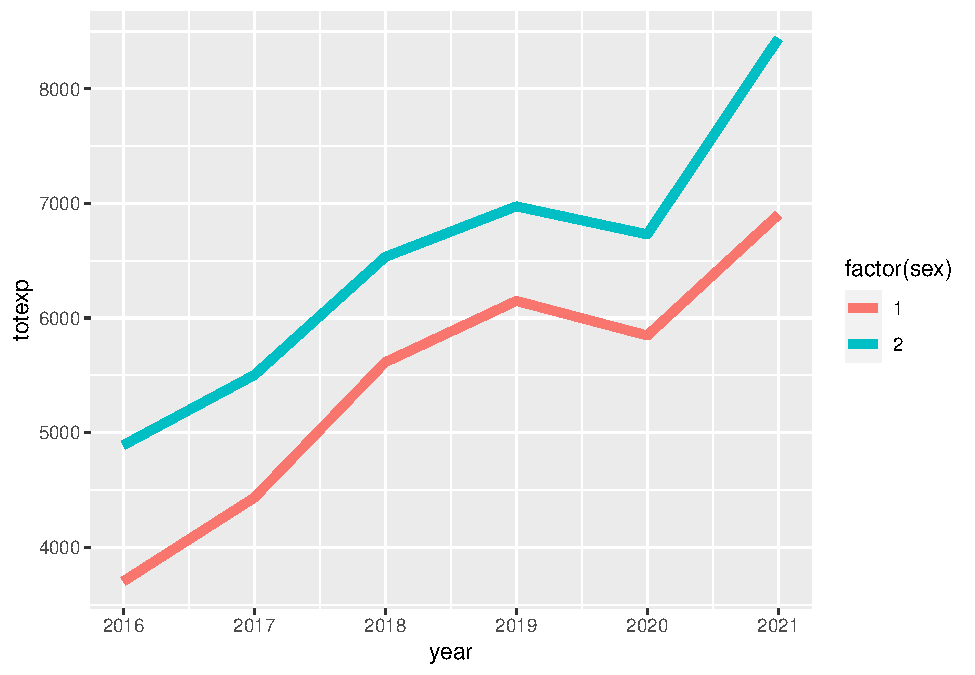
\includegraphics{_main_files/figure-latex/unnamed-chunk-87-1.pdf}

\hypertarget{linear-regression-model}{%
\section{Linear regression model}\label{linear-regression-model}}

We can now construct our linear regression model using the ITSA framework. Because we have survey-weights that need to be applied, we will use the \texttt{svyglm} function. We will have several interaction terms according to the ITSA formula presented above. The triple interaction term (\texttt{factor(period):factor(sex):year}) denotes the difference-in-differences estimation. In other words, it is the difference in total healthcare costs between males and females before and after the intervention was implemented. Think of it as subtracting the difference before and after for males and the difference before and after for females. Thus, we are getting two types of differences or the difference-in-differences.

\begin{itemize}
\item
  \texttt{sex} denotes our grouping variable
\item
  \texttt{period} denotes the binary variable that denotes when the intervention was implemented (\texttt{0\ =\ before}, \texttt{1\ =\ after})
\item
  \texttt{year} denotes the time variable in the model
\end{itemize}

\begin{Shaded}
\begin{Highlighting}[]
\CommentTok{\# ITSA: Triple interaction approach}
\NormalTok{itsa1 }\OtherTok{\textless{}{-}} \FunctionTok{svyglm}\NormalTok{(totexp }\SpecialCharTok{\textasciitilde{}} \FunctionTok{factor}\NormalTok{(sex) }\SpecialCharTok{+} \FunctionTok{factor}\NormalTok{(period) }\SpecialCharTok{+}\NormalTok{ year }\SpecialCharTok{+} \FunctionTok{factor}\NormalTok{(period)}\SpecialCharTok{:}\FunctionTok{factor}\NormalTok{(sex) }\SpecialCharTok{+} \FunctionTok{factor}\NormalTok{(sex)}\SpecialCharTok{:}\NormalTok{year }\SpecialCharTok{+} \FunctionTok{factor}\NormalTok{(period)}\SpecialCharTok{:}\FunctionTok{factor}\NormalTok{(sex)}\SpecialCharTok{:}\NormalTok{year, }\AttributeTok{design =}\NormalTok{ survey\_design) }\DocumentationTok{\#\# ITSA linear model}
\NormalTok{itsa1.confint }\OtherTok{\textless{}{-}} \FunctionTok{confint}\NormalTok{(itsa1) }\DocumentationTok{\#\# generate the 95\% CI}

\CommentTok{\# "cbind" the coefficient output with 95\% CI output}
\FunctionTok{round}\NormalTok{(}
  \FunctionTok{cbind}\NormalTok{(}
    \FunctionTok{summary}\NormalTok{(itsa1, }\AttributeTok{df.resid =} \FunctionTok{degf}\NormalTok{(itsa1}\SpecialCharTok{$}\NormalTok{survey.design))}\SpecialCharTok{$}\NormalTok{coef, }
    \FunctionTok{confint}\NormalTok{(itsa1, }\AttributeTok{df =} \FunctionTok{degf}\NormalTok{(itsa1}\SpecialCharTok{$}\NormalTok{survey.design))}
\NormalTok{  ), }\DecValTok{2}\NormalTok{)}
\end{Highlighting}
\end{Shaded}

\begin{verbatim}
##                                      Estimate Std. Error t value Pr(>|t|)
## (Intercept)                       -1141706.66  227313.30   -5.02     0.00
## factor(sex)2                        156608.67  280182.38    0.56     0.58
## factor(period)1                     638235.37  399815.90    1.60     0.11
## year                                   568.46     112.71    5.04     0.00
## factor(sex)2:factor(period)1       -516623.61  486326.52   -1.06     0.29
## factor(sex)2:year                      -77.08     138.92   -0.55     0.58
## factor(sex)1:factor(period)1:year     -316.27     198.07   -1.60     0.11
## factor(sex)2:factor(period)1:year      -60.45     181.29   -0.33     0.74
##                                         2.5 %     97.5 %
## (Intercept)                       -1588358.77 -695054.56
## factor(sex)2                       -393926.88  707144.22
## factor(period)1                    -147370.28 1423841.03
## year                                   347.00     789.92
## factor(sex)2:factor(period)1      -1472215.58  438968.35
## factor(sex)2:year                     -350.04     195.88
## factor(sex)1:factor(period)1:year     -705.47      72.93
## factor(sex)2:factor(period)1:year     -416.68     295.78
\end{verbatim}

\hypertarget{plot}{%
\section{Plot}\label{plot}}

We can plot our ITSA along with the counterfactuals. We create two new objects \texttt{itsa1} and \texttt{itsa2}, which contain the predicted values from our model. The first object \texttt{itsa1} contains the predictive value with all of our terms including the triple interaction. The second object \texttt{itsa2} contains only the counterfactual terms.

\begin{Shaded}
\begin{Highlighting}[]
\DocumentationTok{\#\#\#\#\#\#\#\#\#\#\#\#\#}
\CommentTok{\# Plot}
\DocumentationTok{\#\#\#\#\#\#\#\#\#\#\#\#\#}
\DocumentationTok{\#\#\# Plot: Part 1 {-} Generate the predictions}
\NormalTok{plot.itsa1 }\OtherTok{\textless{}{-}} \FunctionTok{ggpredict}\NormalTok{(itsa1, }\AttributeTok{terms =} \FunctionTok{c}\NormalTok{(}\StringTok{"year"}\NormalTok{, }\StringTok{"sex"}\NormalTok{, }\StringTok{"period"}\NormalTok{), }\AttributeTok{ci.level =} \FloatTok{0.95}\NormalTok{) }\CommentTok{\# Full model}
\NormalTok{plot.itsa2 }\OtherTok{\textless{}{-}} \FunctionTok{ggpredict}\NormalTok{(itsa1, }\AttributeTok{terms =} \FunctionTok{c}\NormalTok{(}\StringTok{"year"}\NormalTok{, }\StringTok{"sex"}\NormalTok{), }\AttributeTok{ci.level =} \FloatTok{0.95}\NormalTok{) }\CommentTok{\# Counterfactual}


\DocumentationTok{\#\#\# Plot: Part 2 {-} Plot the fitted values}
\CommentTok{\# Start with the scatter (average values at each year by group)}
\NormalTok{colors }\OtherTok{\textless{}{-}} \FunctionTok{c}\NormalTok{(}\StringTok{"darkgreen"}\NormalTok{, }\StringTok{"navyblue"}\NormalTok{) }\CommentTok{\# Create color vector}

\FunctionTok{plot}\NormalTok{(df1}\SpecialCharTok{$}\NormalTok{year, df1}\SpecialCharTok{$}\NormalTok{totexp, }\AttributeTok{pch =} \DecValTok{19}\NormalTok{, }\AttributeTok{cex =} \FloatTok{1.5}\NormalTok{, }\AttributeTok{lwd =} \DecValTok{1}\NormalTok{,}
     \AttributeTok{col =}\NormalTok{ colors[}\FunctionTok{factor}\NormalTok{(df1}\SpecialCharTok{$}\NormalTok{sex)],}
     \AttributeTok{xlab =} \StringTok{"Time (year)"}\NormalTok{, }
     \AttributeTok{ylab =} \StringTok{"Average total healthcare costs ($)"}\NormalTok{,}
     \AttributeTok{ylim =} \FunctionTok{c}\NormalTok{(}\DecValTok{4000}\NormalTok{, }\DecValTok{8000}\NormalTok{))}
\FunctionTok{legend}\NormalTok{(}\StringTok{"topleft"}\NormalTok{, }\AttributeTok{title =} \StringTok{"Groups"}\NormalTok{, }
       \AttributeTok{legend =} \FunctionTok{c}\NormalTok{(}\StringTok{"Male"}\NormalTok{, }\StringTok{"Female"}\NormalTok{),}
       \AttributeTok{fill =} \FunctionTok{c}\NormalTok{(}\StringTok{"darkgreen"}\NormalTok{, }\StringTok{"navyblue"}\NormalTok{))}

\CommentTok{\# Add the lines for the per{-}post index periods}
\FunctionTok{with}\NormalTok{(}\FunctionTok{subset}\NormalTok{(plot.itsa1, x }\SpecialCharTok{\textless{}=} \DecValTok{2019} \SpecialCharTok{\&}\NormalTok{ group }\SpecialCharTok{==} \DecValTok{1} \SpecialCharTok{\&}\NormalTok{ facet }\SpecialCharTok{==} \DecValTok{0}\NormalTok{), }\FunctionTok{lines}\NormalTok{(x, predicted, }\AttributeTok{col =} \StringTok{"darkgreen"}\NormalTok{, }\AttributeTok{lwd =} \DecValTok{2}\NormalTok{))}
\FunctionTok{with}\NormalTok{(}\FunctionTok{subset}\NormalTok{(plot.itsa1, x }\SpecialCharTok{\textless{}=} \DecValTok{2019} \SpecialCharTok{\&}\NormalTok{ group }\SpecialCharTok{==} \DecValTok{2} \SpecialCharTok{\&}\NormalTok{ facet }\SpecialCharTok{==} \DecValTok{0}\NormalTok{), }\FunctionTok{lines}\NormalTok{(x, predicted, }\AttributeTok{col =} \StringTok{"navyblue"}\NormalTok{, }\AttributeTok{lwd =} \DecValTok{2}\NormalTok{))}
\FunctionTok{with}\NormalTok{(}\FunctionTok{subset}\NormalTok{(plot.itsa1, x }\SpecialCharTok{\textgreater{}=} \DecValTok{2019} \SpecialCharTok{\&}\NormalTok{ group }\SpecialCharTok{==} \DecValTok{1} \SpecialCharTok{\&}\NormalTok{ facet }\SpecialCharTok{==} \DecValTok{1}\NormalTok{), }\FunctionTok{lines}\NormalTok{(x, predicted, }\AttributeTok{col =} \StringTok{"darkgreen"}\NormalTok{, }\AttributeTok{lwd =} \DecValTok{2}\NormalTok{))}
\FunctionTok{with}\NormalTok{(}\FunctionTok{subset}\NormalTok{(plot.itsa1, x }\SpecialCharTok{\textgreater{}=} \DecValTok{2019} \SpecialCharTok{\&}\NormalTok{ group }\SpecialCharTok{==} \DecValTok{2} \SpecialCharTok{\&}\NormalTok{ facet }\SpecialCharTok{==} \DecValTok{1}\NormalTok{), }\FunctionTok{lines}\NormalTok{(x, predicted, }\AttributeTok{col =} \StringTok{"navyblue"}\NormalTok{, }\AttributeTok{lwd =} \DecValTok{2}\NormalTok{))}

\CommentTok{\# Line for the index period}
\FunctionTok{abline}\NormalTok{(}\AttributeTok{v =} \DecValTok{2019}\NormalTok{, }\AttributeTok{col =} \StringTok{"red"}\NormalTok{, }\AttributeTok{lty =} \DecValTok{2}\NormalTok{, }\AttributeTok{lwd =} \DecValTok{2}\NormalTok{)}

\CommentTok{\# Counterfactual lines}
\FunctionTok{with}\NormalTok{(}\FunctionTok{subset}\NormalTok{(plot.itsa2, x }\SpecialCharTok{\textgreater{}=} \DecValTok{2019} \SpecialCharTok{\&}\NormalTok{ group }\SpecialCharTok{==} \DecValTok{1}\NormalTok{), }\FunctionTok{lines}\NormalTok{(x, predicted, }\AttributeTok{col =} \StringTok{"darkgreen"}\NormalTok{, }\AttributeTok{lty =} \DecValTok{2}\NormalTok{, }\AttributeTok{lwd =} \DecValTok{2}\NormalTok{))}
\FunctionTok{with}\NormalTok{(}\FunctionTok{subset}\NormalTok{(plot.itsa2, x }\SpecialCharTok{\textgreater{}=} \DecValTok{2019} \SpecialCharTok{\&}\NormalTok{ group }\SpecialCharTok{==} \DecValTok{2}\NormalTok{), }\FunctionTok{lines}\NormalTok{(x, predicted, }\AttributeTok{col =} \StringTok{"navyblue"}\NormalTok{, }\AttributeTok{lty =} \DecValTok{2}\NormalTok{, }\AttributeTok{lwd =} \DecValTok{2}\NormalTok{))}
\end{Highlighting}
\end{Shaded}

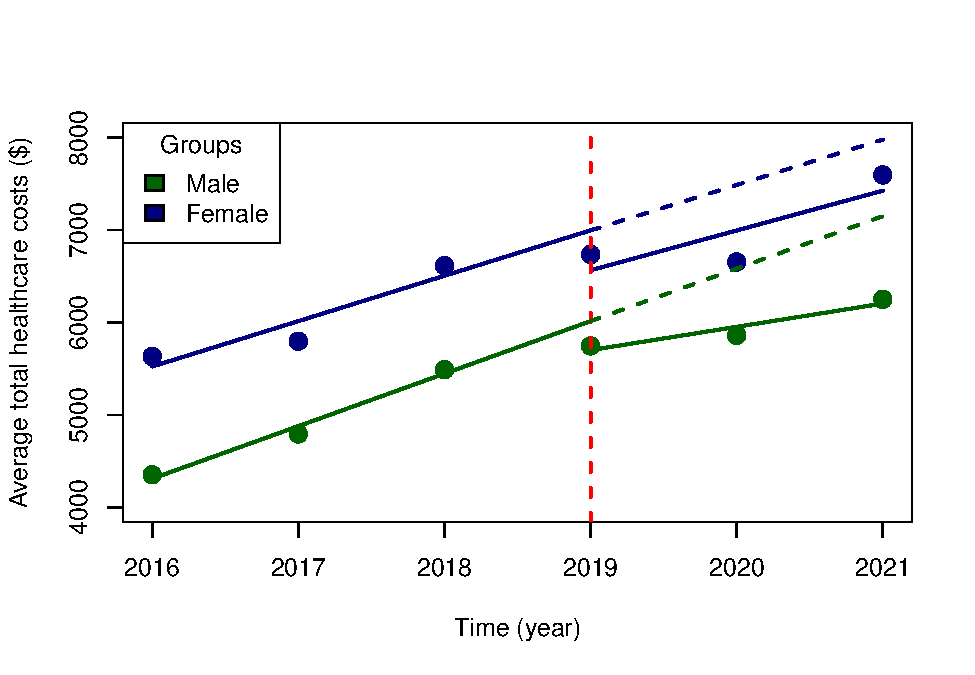
\includegraphics{_main_files/figure-latex/unnamed-chunk-89-1.pdf}

\hypertarget{parallel-trends-assumption}{%
\section{Parallel trends assumption}\label{parallel-trends-assumption}}

The most critical part of the ITSA results are the parallel trends assumption and the difference-in-differences estimator.

Let's start with the parallel trends assumption. We need to test to see if the trends between males and females are similar before the implementation of the intervention, which we can find in our model output. Based on our findings (see \texttt{factor(sex)2:year} coefficient), the slopes between the two groups (males and females) before the intervention were not statistically different (average difference = -\$77 (95\% CI: -\$350, \$196). This means that the slopes are not significantly different between males and females. See ITSA Figure below with annotations.

Once we are confident that the trends prior to the implementation of the intervention are not different, any changes we see after the intervention can be attributed to the intervention. This is an important condition for the difference-in-differences design.

\hypertarget{additional-estimations}{%
\section{Additional estimations}\label{additional-estimations}}

We can use the \texttt{margins} command to estimate the partial derivatives of the total healthcare costs along different parts of the timeline.

For instance, the average difference in total healthcare costs for males and females before and after the intervention were \$1020 and \$777, respectively. I've summarized these results into a table below.

\begin{Shaded}
\begin{Highlighting}[]
\DocumentationTok{\#\#\# Average difference total costs in the pre{-} and post{-}intervention periods. }
\NormalTok{margins1 }\OtherTok{\textless{}{-}} \FunctionTok{margins}\NormalTok{(itsa1, }\AttributeTok{type =} \StringTok{"response"}\NormalTok{, }\AttributeTok{design =}\NormalTok{ survey\_design, }\AttributeTok{at =}\NormalTok{ (}\FunctionTok{list}\NormalTok{(}\AttributeTok{period =} \DecValTok{0}\SpecialCharTok{:}\DecValTok{1}\NormalTok{)), }\AttributeTok{variables =} \StringTok{"sex"}\NormalTok{)}
\FunctionTok{summary}\NormalTok{(margins1)}
\end{Highlighting}
\end{Shaded}

\begin{verbatim}
##  factor period       AME       SE      z      p    lower     upper
##    sex2 0.0000 1020.3870 251.0666 4.0642 0.0000 539.0557 1523.2188
##    sex2 1.0000  777.3969 260.7194 2.9817 0.0029 241.4676 1263.4687
\end{verbatim}

\begin{figure}
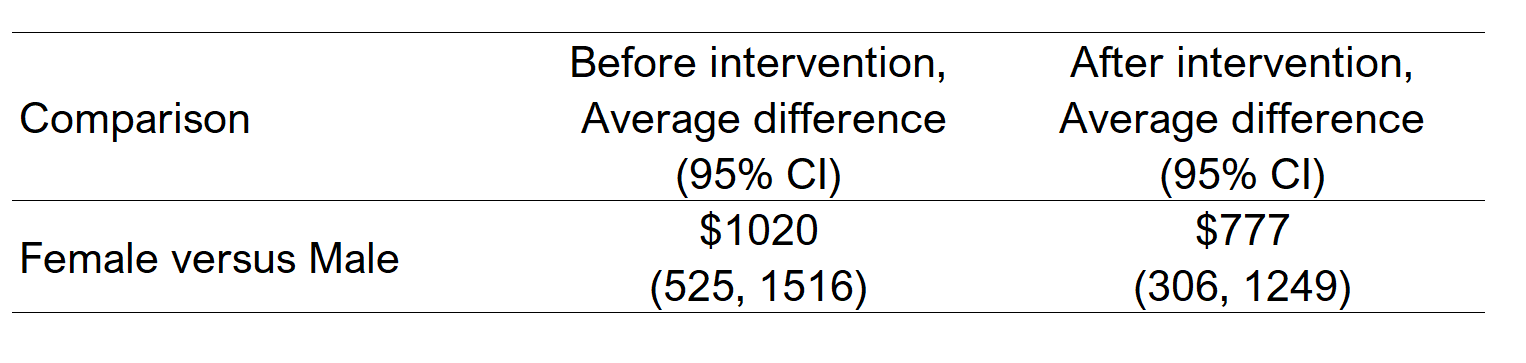
\includegraphics[width=1\linewidth]{Figure 6_2} \caption{Differences in total healthcare costs between males and females.}\label{fig:unnamed-chunk-91}
\end{figure}

We could also estimate the slopes or the average annual change in the total healthcare costs for males and females after the intervention using the \texttt{margins} commands. For instance, average annual change in total healthcare costs for males and females are \$252 and \$431, respectively.

\begin{Shaded}
\begin{Highlighting}[]
\DocumentationTok{\#\#\# Slopes after the intervention}
\NormalTok{margins3 }\OtherTok{\textless{}{-}} \FunctionTok{margins}\NormalTok{(itsa1, }\AttributeTok{type =} \StringTok{"response"}\NormalTok{, }\AttributeTok{design =}\NormalTok{ survey\_design, }\AttributeTok{at =}\NormalTok{ (}\FunctionTok{list}\NormalTok{(}\AttributeTok{period =} \DecValTok{1}\NormalTok{, }\AttributeTok{sex =}\NormalTok{ (}\DecValTok{1}\SpecialCharTok{:}\DecValTok{2}\NormalTok{))), }\AttributeTok{variables =} \StringTok{"year"}\NormalTok{)}
\FunctionTok{summary}\NormalTok{(margins3)}
\end{Highlighting}
\end{Shaded}

\begin{verbatim}
##  factor period    sex      AME       SE      z      p    lower    upper
##    year 1.0000 1.0000 252.1903 151.9225 1.6600 0.0969 -45.5724 549.9530
##    year 1.0000 2.0000 430.9319 134.2015 3.2111 0.0013 167.9019 693.9620
\end{verbatim}

\hypertarget{issues-with-the-current-model}{%
\section{Issues with the current model}\label{issues-with-the-current-model}}

However, it is not possible to compare the slopes using the \texttt{R} version of the \texttt{margins} package. I have tried to search for a way to do this, but the \texttt{margins} package for \texttt{R} currently can't perform this comparison. You can follow the discussion on the \texttt{margins} GitHub page (\href{https://github.com/leeper/margins/issues/124}{link}), which discusses some potential solution. However, I prefer to use \texttt{Stata} for these comparisons. Fortunately, there is a way to make some important conclusions using a different method--the linear spline model.

\hypertarget{workaround-using-a-linear-spline-model}{%
\section{Workaround using a linear spline model}\label{workaround-using-a-linear-spline-model}}

We could get the difference in the level change immediately after implementation of the intervention at \texttt{year\ ==\ 2019} using the \texttt{lspline} command. We can also get the difference-in-differences estimate with this approach.

\begin{Shaded}
\begin{Highlighting}[]
\CommentTok{\# ITSA: Linear splines approach}
\DocumentationTok{\#\#\# Create a knot at 2019}
\NormalTok{spline1 }\OtherTok{\textless{}{-}} \FunctionTok{svyglm}\NormalTok{(totexp }\SpecialCharTok{\textasciitilde{}} \FunctionTok{factor}\NormalTok{(sex) }\SpecialCharTok{+} \FunctionTok{factor}\NormalTok{(period) }\SpecialCharTok{+} \FunctionTok{lspline}\NormalTok{(year, }\FunctionTok{c}\NormalTok{(}\DecValTok{2019}\NormalTok{), }\AttributeTok{marginal =} \ConstantTok{TRUE}\NormalTok{) }\SpecialCharTok{+} \FunctionTok{factor}\NormalTok{(sex)}\SpecialCharTok{:}\FunctionTok{lspline}\NormalTok{(year, }\FunctionTok{c}\NormalTok{(}\DecValTok{2019}\NormalTok{), }\AttributeTok{marginal =} \ConstantTok{TRUE}\NormalTok{) }\SpecialCharTok{+} \FunctionTok{factor}\NormalTok{(sex)}\SpecialCharTok{:}\FunctionTok{factor}\NormalTok{(period), }\AttributeTok{design =}\NormalTok{ survey\_design)}
\NormalTok{spline1.confint }\OtherTok{\textless{}{-}} \FunctionTok{confint}\NormalTok{(spline1)}

\CommentTok{\# Output with 95\% CI}
\FunctionTok{round}\NormalTok{(}
  \FunctionTok{cbind}\NormalTok{(}
    \FunctionTok{summary}\NormalTok{(spline1, }\AttributeTok{df.resid =} \FunctionTok{degf}\NormalTok{(spline1}\SpecialCharTok{$}\NormalTok{survey.design))}\SpecialCharTok{$}\NormalTok{coef, }
    \FunctionTok{confint}\NormalTok{(spline1, }\AttributeTok{df =} \FunctionTok{degf}\NormalTok{(spline1}\SpecialCharTok{$}\NormalTok{survey.design))}
\NormalTok{  ), }\DecValTok{2}\NormalTok{)}
\end{Highlighting}
\end{Shaded}

\begin{verbatim}
##                                                          Estimate Std. Error
## (Intercept)                                           -1141706.66  227313.30
## factor(sex)2                                            156608.67  280182.38
## factor(period)1                                           -313.65     285.65
## lspline(year, c(2019), marginal = TRUE)1                   568.46     112.71
## lspline(year, c(2019), marginal = TRUE)2                  -316.27     198.07
## factor(sex)2:lspline(year, c(2019), marginal = TRUE)1      -77.08     138.92
## factor(sex)2:lspline(year, c(2019), marginal = TRUE)2      255.82     240.93
## factor(sex)2:factor(period)1                              -118.53     370.05
##                                                       t value Pr(>|t|)
## (Intercept)                                             -5.02     0.00
## factor(sex)2                                             0.56     0.58
## factor(period)1                                         -1.10     0.27
## lspline(year, c(2019), marginal = TRUE)1                 5.04     0.00
## lspline(year, c(2019), marginal = TRUE)2                -1.60     0.11
## factor(sex)2:lspline(year, c(2019), marginal = TRUE)1   -0.55     0.58
## factor(sex)2:lspline(year, c(2019), marginal = TRUE)2    1.06     0.29
## factor(sex)2:factor(period)1                            -0.32     0.75
##                                                             2.5 %     97.5 %
## (Intercept)                                           -1588358.77 -695054.56
## factor(sex)2                                           -393926.88  707144.22
## factor(period)1                                           -874.93     247.63
## lspline(year, c(2019), marginal = TRUE)1                   347.00     789.92
## lspline(year, c(2019), marginal = TRUE)2                  -705.47      72.93
## factor(sex)2:lspline(year, c(2019), marginal = TRUE)1     -350.04     195.88
## factor(sex)2:lspline(year, c(2019), marginal = TRUE)2     -217.59     729.23
## factor(sex)2:factor(period)1                              -845.64     608.58
\end{verbatim}

The linear spline model creates \texttt{knots} that automatically replaces some of the interactions in our previous model. For example the model element \texttt{factor(sex):lspline(year,\ c(2019)} replaces the triple interaction \texttt{factor(period):factor(sex):year} from our previous model.

You'll notice that some of the coefficient values are similar to our first model. For instance, in our first model, the \texttt{year} coefficient was equal to \$568, and in the linear splines model, the \texttt{lspline(year,\ c(2019),\ marginal\ =\ TRUE)1} coefficient was equal to \$568. This denotes the average change in annual total healthcare costs for males before the implementation of the intervention at \texttt{year\ ==\ 2019}.

However, you'll also notice some differences. In the linear splines model, we have a couple of important coefficients that will help to complete our evaluation of the ITSA model.

\hypertarget{differences-in-level-immediately-after-implementation-of-the-intervention}{%
\section{Differences in level immediately after implementation of the intervention}\label{differences-in-level-immediately-after-implementation-of-the-intervention}}

One of the most important changes we are interested in is the \emph{immediate} change after implementation of the intervention at \texttt{year\ ==\ 2019}. This is captured with the \texttt{factor(sex)2:factor(period)1} coefficient, which has a value equal to -\$119 (95\% CI: -\$846, \$609). This tells me that the difference in level change at \texttt{year\ ==\ 2019} was lower for females than males; however, this difference was not statistically significant. See ITSA Figure below with annotations.

\hypertarget{difference-in-differences-estimation}{%
\section{Difference-in-differences estimation}\label{difference-in-differences-estimation}}

Lastly, we can identify the difference-in-differences estimate from the linear spline model output in the form of the \texttt{factor(sex)2:lspline(year,\ c(2019),\ marginal\ =\ TRUE)2} coefficient, which has a value equal to \$256 (95\% CI: -\$218, \$729). This coefficient denotes that average annual change in total healthcare expenditure between males and females before and after implementation of the intervention. In other words, this is a difference in the slopes for males before and after the intervention minus the difference in the slopes for females before and after the intervention. Hence, the term \texttt{difference-in-differences}. See ITSA Figure below with annotations.

\begin{figure}
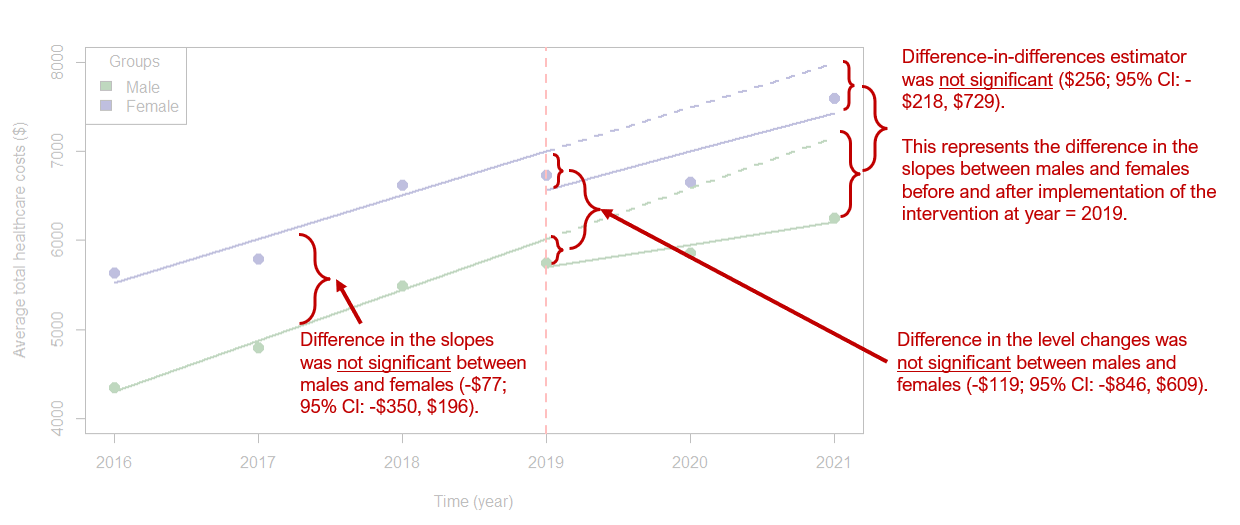
\includegraphics[width=1\linewidth]{Figure 6_3} \caption{ITSA figure with annotations.}\label{fig:unnamed-chunk-94}
\end{figure}

\hypertarget{putting-it-all-together}{%
\section{Putting it all together}\label{putting-it-all-together}}

With the ITSA, we will summarize our findings into a table. These include the main coefficients from the ITSA model.

\begin{figure}
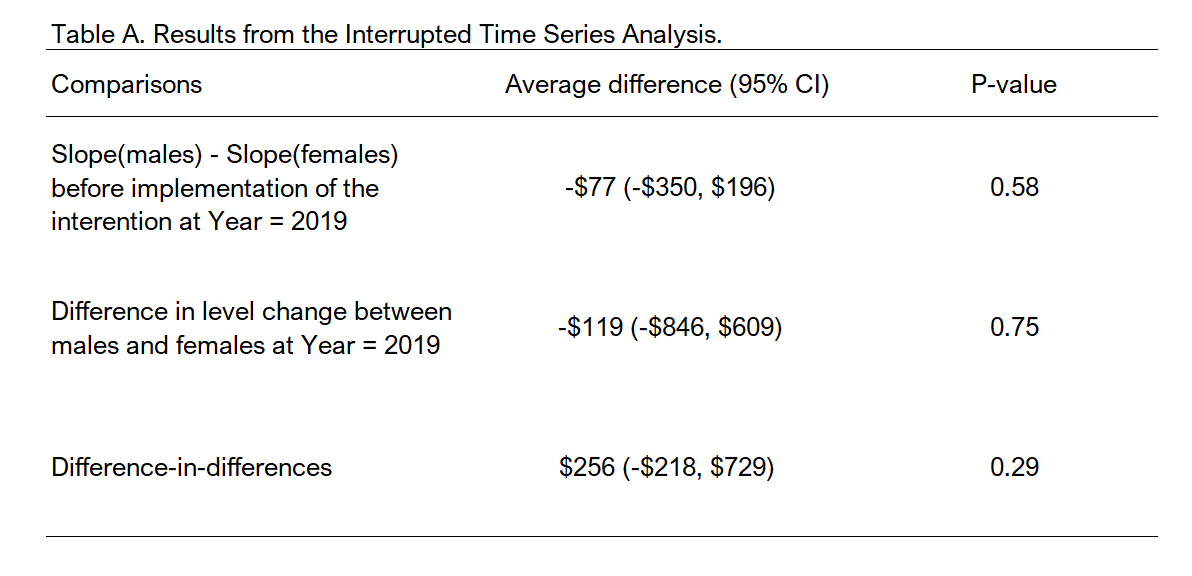
\includegraphics[width=1\linewidth]{Figure 6_4} \caption{Summary table for main ITSA coefficients.}\label{fig:unnamed-chunk-95}
\end{figure}

\hypertarget{conclusions-5}{%
\section{Conclusions}\label{conclusions-5}}

The ITSA model is a very useful design to generate causal interpretation as long as the assumptions hold. For instance, the parallel trends assumptions needs to be assessed. Without it, it will be difficult to argue that the intervention was the only factor that could have impacted the changes in the level and trends between the groups.

In this tutorial, I ran into an issue with the first ITSA model using interaction terms. It didn't provide me with the necessary coefficients to determine the main coefficients for the ITSA. For instance, I had to use a linear spline model to identify the difference-in-differences estimate. Although the ITSA model with the triple interaction was useful in generating the plot, I could have started with the linear splines model and generated the ITSA plot afterwards with the triple interaction model.

At the end of the day, I was able to generate a summary table and a very nice figure of the ITSA. However, I will continue to learn more about other contrasting packages such as \href{https://github.com/rvlenth/emmeans}{\texttt{emmeans}} and \href{https://github.com/vincentarelbundock/marginaleffects}{\texttt{marginaleffects}}.

Although the \texttt{margins} package in \texttt{R} doesn't have the \texttt{pwcompare} feature from \texttt{Stata}, there are some potential workarounds that I'll investigate further. Discussion about this can be found in the \texttt{margins} GitHub issues forum (\href{https://github.com/leeper/margins/issues/124}{link})

\hypertarget{acknowledgements-5}{%
\section{Acknowledgements}\label{acknowledgements-5}}

As always, I am grateful to the \texttt{R} community for producing wonderful tools for novices like me. I've learned so much reading documents, forums, and issues online that it would be impossible to credit everyone. But I would like to highlight a few superstars that I think deserve special recognition.

I am grateful to the author of the \texttt{margins} package, Thomas J. Leeper. You can find his \texttt{margins} package on his \href{https://github.com/leeper/margins}{\texttt{GitHub\ site}}.

Additionally, the \texttt{marginaleffects} package by Vincent Arel-Bundock has helped me to compare some of \texttt{R}'s marginal effects commands with \texttt{Stata}. You can find his GitHub site \href{https://github.com/vincentarelbundock/marginaleffects}{here}.

The \texttt{emmeans} package was developed by Russel V. Length, which I plan on learning more about on his GitHub site (\href{https://github.com/rvlenth/emmeans}{link}). Note: I found a nice overview of the \texttt{emmeans} package by Ariel Muldoon that I encourage interested users to read (\href{https://aosmith.rbind.io/2019/03/25/getting-started-with-emmeans/}{link}).

The \texttt{ggeffect} package was very useful in helping me develop some very nice plots, which you can learn more about on their GitHub site (\href{https://strengejacke.github.io/ggeffects/}{link}).

Lastly, I found this amazing site on ITSA by Chrissy H. Roberts \href{https://rpubs.com/chrissyhroberts/1006858}{here}. Her site helped me to create the ITSA plot which is in this tutorial. I hope you get a chance to read her blog on how to conduct an ITSA in R. I think she does a much better job that I did with this tutorial.

\hypertarget{work-in-progress-2}{%
\section{Work in progress}\label{work-in-progress-2}}

This is a work in progress so expect some updates in the future.

\hypertarget{disclaimers-2}{%
\section{Disclaimers}\label{disclaimers-2}}

Any errors or mistakes are those of the author.

This is only for educational purposes.

This was built under R version 4.3.1 ``Beagle Scouts''

\hypertarget{notes}{%
\chapter{Helpful Notes}\label{notes}}

\hypertarget{introduction-6}{%
\section{Introduction}\label{introduction-6}}

There are several things that I've learned while exploring and using the Agency for Health Research and Quality (AHRQ) Medical Expenditure Panel Survey (MEPS) data. Although there are (very good) documentations provided by AHRQ MEPS, I thought I would write a short article about some of the (``hard'') lessons I learned.

In this article, I summarize some of these lessons in no particular order. I may expand on this list as time goes on, but for now, I will start off with a few of these.

\hypertarget{meps-file-names}{%
\subsection{1. MEPS file names}\label{meps-file-names}}

AHRQ MEPS has a \href{https://github.com/HHS-AHRQ/MEPS/tree/master}{GitHub site} with a lot of resources. One of the most useful resource is a list of their MEPS files. This list contains the MEPS file names, which are used to identify the data for import using the \texttt{MEPS} package.

For example, we can use the \texttt{read\_MEPS()} function to import the MEPS file of interest (Note: Make sure you have an internet connection). The file name for the 2021 Full-Year Consolidated File is \texttt{"h233"}.

\begin{Shaded}
\begin{Highlighting}[]
\DocumentationTok{\#\#\# Load MEPS library}
\FunctionTok{library}\NormalTok{(}\StringTok{"MEPS"}\NormalTok{)}

\DocumentationTok{\#\#\# Import the 2021 Full Year Consolidated File}
\NormalTok{hc2021 }\OtherTok{=} \FunctionTok{read\_MEPS}\NormalTok{(}\AttributeTok{file =} \StringTok{"h233"}\NormalTok{) }\CommentTok{\# Full{-}year consolidated file}
\end{Highlighting}
\end{Shaded}

You can find the list of the MEPS file names \href{https://github.com/HHS-AHRQ/MEPS/blob/master/Quick_Reference_Guides/meps_file_names.csv}{here}.

Here is an example of some of the file codes:

\begin{figure}
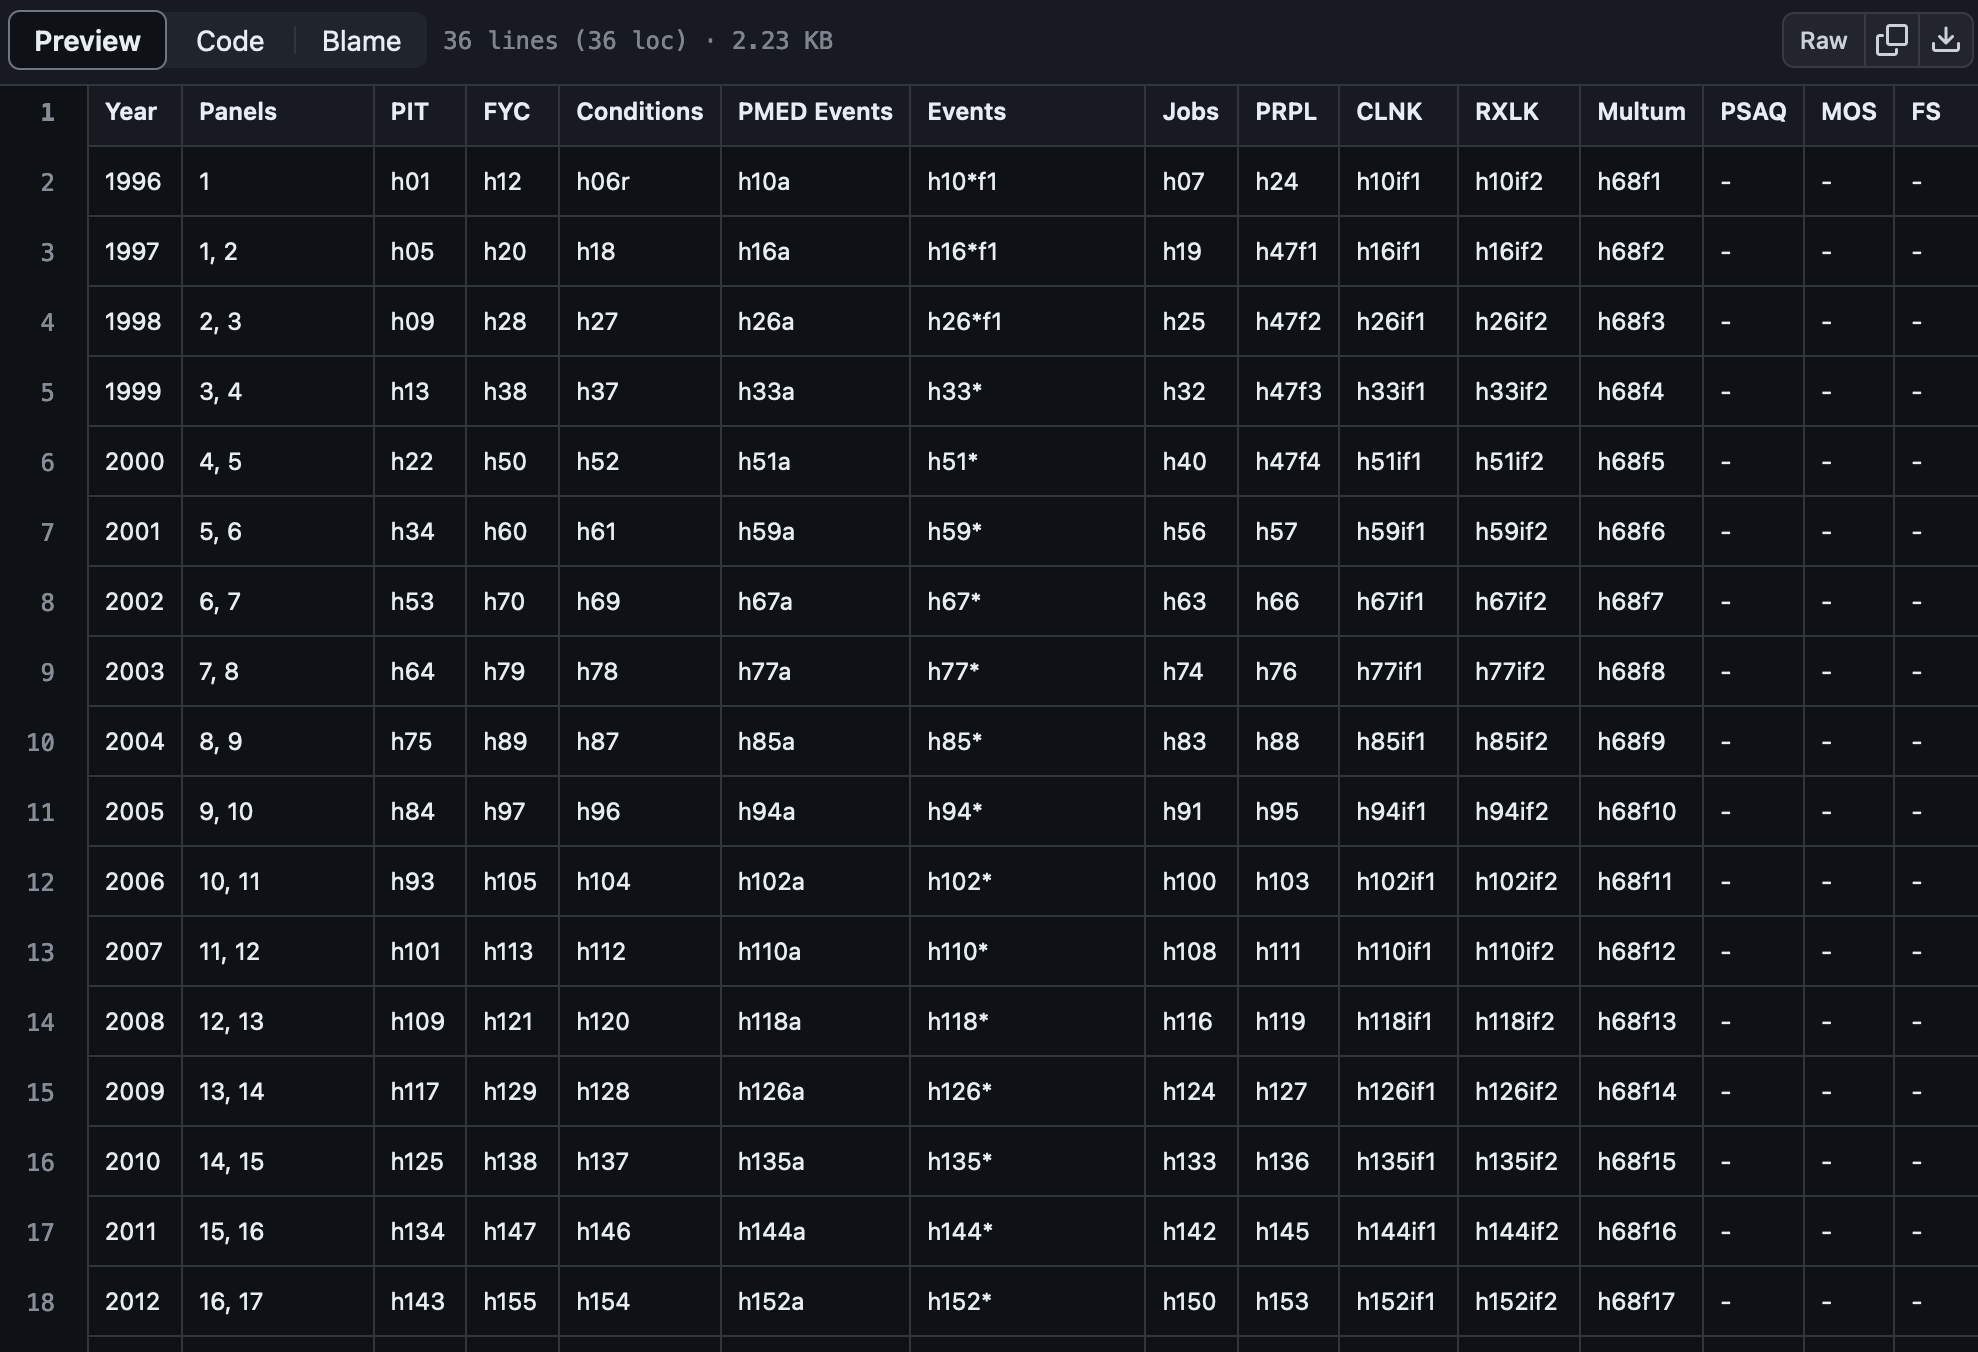
\includegraphics[width=1\linewidth]{Figure 7_2 - MEPS - File codes} \caption{Figure - MEPS file codes example.}\label{fig:unnamed-chunk-97}
\end{figure}

\hypertarget{expenditure-categories}{%
\subsection{2. Expenditure categories}\label{expenditure-categories}}

MEPS contains a ton of expenditure categories such as outpatient and inpatient. This is helpful when you want to \textbf{deconstruct} the total expenditures into its different components.

Here is a list of the various expenditure categories from the \href{https://meps.ahrq.gov/data_stats/download_data/pufs/h233/h233doc.shtml}{2021 Full Year Consolidated file}.

\begin{figure}
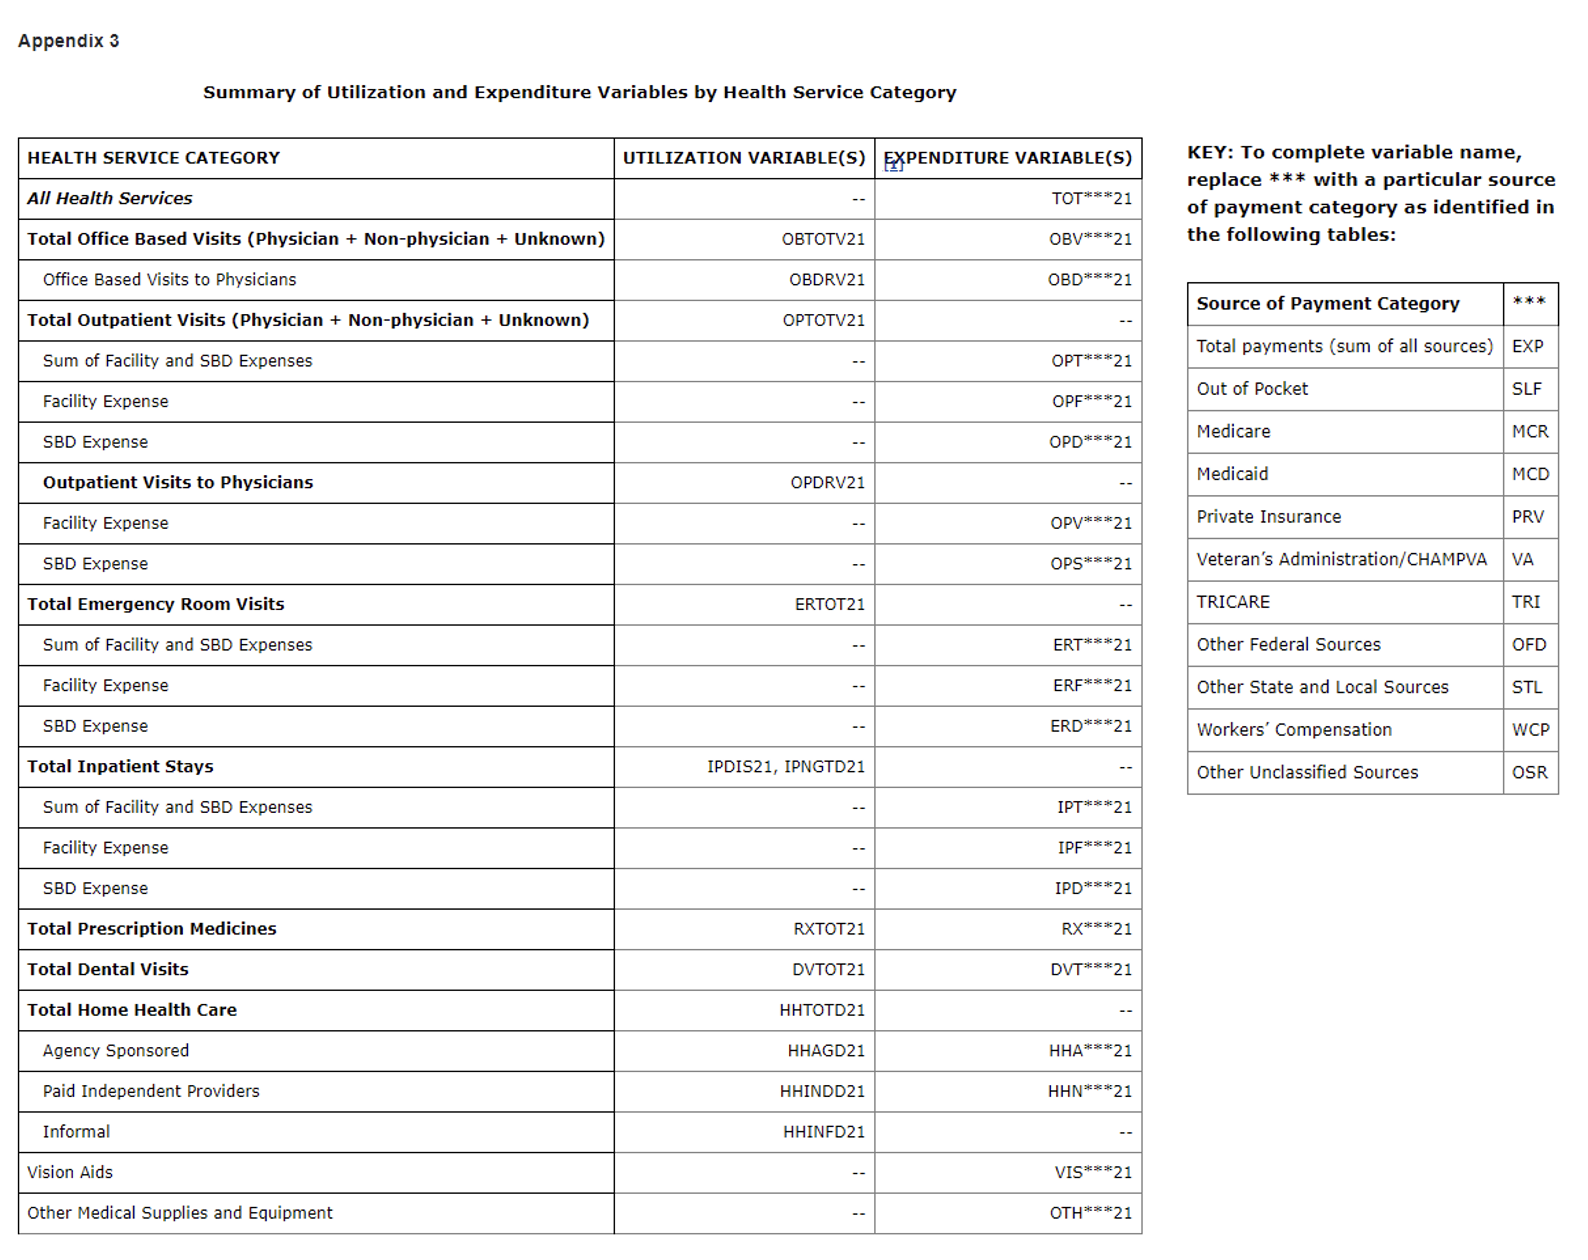
\includegraphics[width=1\linewidth]{Figure 7_1 - MEPS - Appendix 3} \caption{Figure - MEPS expenditure categories.}\label{fig:unnamed-chunk-98}
\end{figure}

\hypertarget{example-expenditure-categories}{%
\subsubsection{2.1. Example expenditure categories}\label{example-expenditure-categories}}

For example, the 2021 annual costs variable for office-based visits is \texttt{OBVEXP21}. Each of these expenditure categories represent different areas of care that an individual can access. I provide a summary of a select few.

\begin{itemize}
\item
  \texttt{OBVEXP21} denotes the office-based visits costs for 2021. These include encounters that are provided in the physician's office or clinic setting. It does not include encounters associated with the hospital, nursing home, or patient's home.
\item
  \texttt{OBTOTV21} denotes the number of office-based visits in 2021.
\item
  \texttt{OPTEXP21} denotes the outpatient visit costs for 2021. These include encounters in hospital's outpatient departments. The total costs for an outpatient visit contains the facility and ``SBD'' expenses. (Note: ``SBD'' is short for ``separate billing doctor'' and refers to physicians who are billed separately for services provided at the hospital or site. They are not included in the facility-only costs.)
\item
  \texttt{ERTEXP21} denotes the emergency department visit costs for 2021. Emergency department visit that result in an inpatient stay are ``rolled'' up into the inpatient costs. You should be aware that ``double-counting'' can occur as a consequence of this ``roll-up.'' MEPS handles this by assigning \$0 to the emergency department facility costs. Physician costs and the number of emergency department visits are not affect by this ``roll-up'' issue.
\item
  \texttt{ERTOT21} denotes the number of emergency room visits in 2021.
\item
  \texttt{IPTEXP21} denotes the inpatient visit costs for 2021. Inpatient visit costs include the facility and SBD costs.
\item
  \texttt{IPDIS21} denotes the number of hospital discharges.
\item
  \texttt{IPNGTD21} denotes the number of nights associated with hospital discharges.
\item
  \texttt{RXEXP21} denotes the total medication costs for 2021. These costs include payments by insurers, health plan benefits, public (Medicare and Medicaid), VA, and out-of-pocket costs.
\item
  \texttt{RXTOT21} denotes the number of prescription fills and refills for 2021.
\end{itemize}

\hypertarget{sources-of-payments}{%
\subsection{3. Sources of payments}\label{sources-of-payments}}

Each expenditure is composed of various sources of payments. Some a mostly composed of public or private payers. Some are mostly out-of-pocket payments. MEPS breaks these down into many parts, the sum of which should equal the total expenditures.

\hypertarget{example-of-sources-of-payments}{%
\subsubsection{3.1. Example of sources of payments}\label{example-of-sources-of-payments}}

In Appendix 3, the \texttt{***} that are listed in the expenditure categories as placeholders for the source of payment codes. These codes are listed in the Figure above. For example, the code for total payments is \texttt{EXP}, and the code for out-of-pocket payments is \texttt{SLF} or self. Thus, the total payments for emergency department visits in 2021 is \texttt{ERTEXP21}, and the out-of-pocket payments for total prescription medicines in 2021 is \texttt{RXSLF21}.

Below is an illustration on how to match expenditure variable codes with the source of payment codes.

\begin{figure}
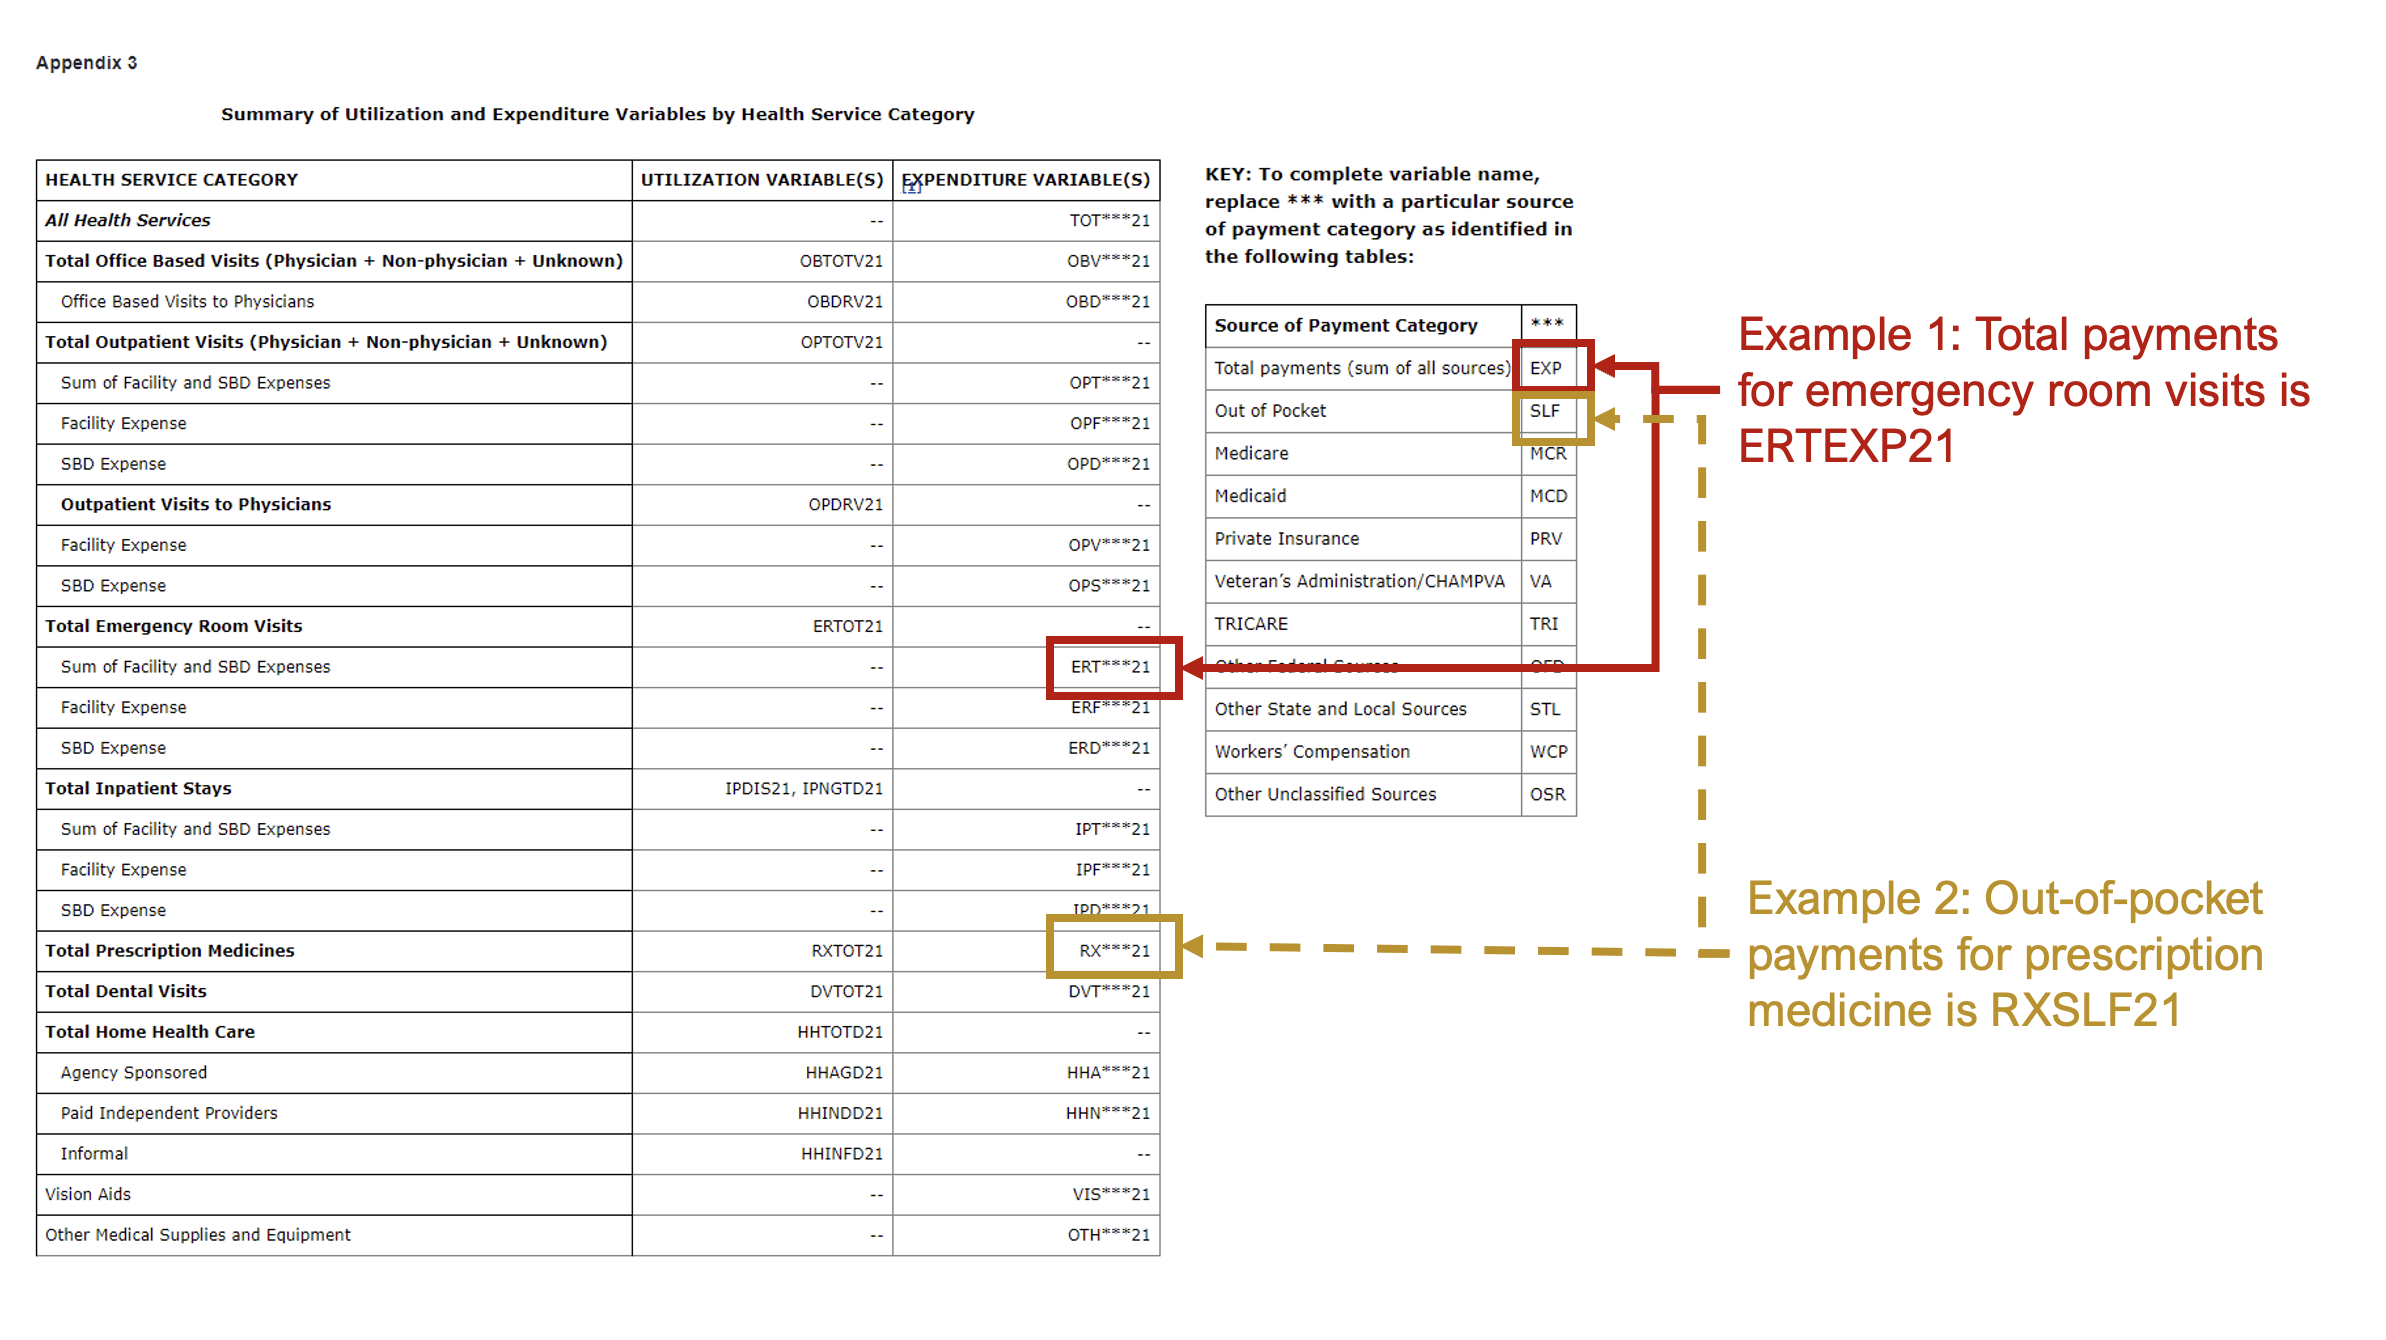
\includegraphics[width=1\linewidth]{Figure 7_3 - MEPS - codes files match} \caption{Figure - MEPS expenditure categories.}\label{fig:unnamed-chunk-99}
\end{figure}

\hypertarget{references}{%
\section{References}\label{references}}

Most of the information can be found on the AHRQ MEPS \href{https://meps.ahrq.gov/mepsweb/}{website}. I encourage the learner to read through the documentations for each data file. It's rich with useful information.

Another great resource is the AHRQ MEPS GitHub \href{https://github.com/HHS-AHRQ/MEPS}{page}. There are example codes on how to use the MEPS data based on R, Stata, and SAS.

\hypertarget{disclaimer}{%
\section{Disclaimer}\label{disclaimer}}

I plan to update this as I learn more about MEPS data, so stay tuned.

This is for educational purposes only.

  \bibliography{book.bib,packages.bib}

\end{document}
